% =====================================================================
%  results_c7.tex
%  Campaign 7: the controllability screen. Section for results.tex,
%  to be pasted after \label{sec:res-c6-compare} closes (line 1992 at
%  the current head) or % =====================================================================
%  results_c7.tex
%  Campaign 7: the controllability screen. Section for results.tex,
%  to be pasted after \label{sec:res-c6-compare} closes (line 1992 at
%  the current head) or % =====================================================================
%  results_c7.tex
%  Campaign 7: the controllability screen. Section for results.tex,
%  to be pasted after \label{sec:res-c6-compare} closes (line 1992 at
%  the current head) or % =====================================================================
%  results_c7.tex
%  Campaign 7: the controllability screen. Section for results.tex,
%  to be pasted after \label{sec:res-c6-compare} closes (line 1992 at
%  the current head) or \input{results_c7} at that point.
%
%  Figures: copy the eight PDF files of c7_analysis_60/ into images/.
%    c7_pareto_60, c7_ctrl_screen, c7_rod_worth, c7_rodded_peaking,
%    c7_kinf_histories, c7_cycle_uncertainty, c7_infill_diversity,
%    c7_vars_influence
%
%  Labels defined here: sec:res-c7, sec:res-c7-basis, sec:res-c7-blocks,
%  sec:res-c7-screens, sec:res-c7-worth, sec:res-c7-rodded,
%  sec:res-c7-uncertainty, sec:res-c7-cost, sec:res-c7-limits,
%  tab:c7-blocks, tab:c7-front, tab:c7-nesting, tab:c7-uncertainty,
%  fig:c7-diversity, fig:c7-screens, fig:c7-pareto, fig:c7-worth,
%  fig:c7-influence, fig:c7-rodded, fig:c7-histories, fig:c7-uncertainty,
%  eq:g-ctrl, eq:k-implied, eq:bank-worth, eq:sigma-beoc, eq:sigma-efpd
%
%  Labels used from elsewhere: sec:meth-ctrl, sec:meth-ktarget,
%  sec:meth-acq, sec:res-c6, sec:res-c6-blocks, tab:fidelity,
%  sec:meth-lax, sec:res-c8, sec:meth-cost. Define sec:meth-ctrl,
%  sec:meth-lax and sec:meth-cost with methodology_c78_additions.tex.
%
%  Style: short paragraphs, no semicolons, no em dashes, every displayed
%  formula followed by a term list with units, enumerations as lists.
% =====================================================================

\section{Campaign 7: the controllability screen}
\label{sec:res-c7}

Campaign 6 closed with a front whose long-cycle end rode the
reactivity ceiling, and with the observation that the ceiling of 1.35
proxied controllable excess reactivity without a rod model. Campaign 7
replaces the proxy by a measurement. Every evaluation now solves the
beginning-of-life core a second time with the sixteen regulating-bank
control rod assemblies inserted, and the resulting eigenvalue enters the
constraint set directly. The campaign ran 60 evaluations on the AWS
instance in \SI{15.82}{h}, and every one of them completed without
error.

\subsection{The one change and its two consequences}
\label{sec:res-c7-basis}

The constraint added is the controllability screen of
Section~\ref{sec:meth-ctrl}.

\begin{equation}
g_\mathrm{ctrl}(\mathbf{x}) = k_\mathrm{ARI}(\mathbf{x}) - (1 - \Delta\rho_\mathrm{op}) \le 0
\label{eq:g-ctrl}
\end{equation}

\noindent where the symbols have the following meaning.

\begin{itemize}
  \item $k_\mathrm{ARI}$ is the effective multiplication factor of the
        32-assembly core at beginning of life with all sixteen
        regulating-bank assemblies inserted and the shutdown banks
        withdrawn, dimensionless.

  \item $\Delta\rho_\mathrm{op}$ is the operating subcriticality margin
        demanded of the regulating banks, \num{0.01} in units of $k$,
        that is \SI{1000}{pcm}.

  \item $\mathbf{x}$ is the design vector.
\end{itemize}

Two settings changed with it. The reactivity ceiling was lowered from
1.35 to 1.126, a value derived before the campaign from the smallest
regulating-bank worth measured on eight Campaign 6 designs, and the
enrichment cap was lowered to \SI{12}{wt\%} on the as-built peripheral
ring, giving a search box of 3.0 to \SI{10.43}{wt\%}. Both were
intended as consequences of the controllability requirement rather than
as independent changes, and the campaign tests whether they were
consistent with the measurement they were meant to anticipate.

\subsection{Design of experiments and the three infill blocks}
\label{sec:res-c7-blocks}

The campaign ran a design of experiments of 42 followed by three infill
blocks of six. Table~\ref{tab:c7-blocks} records the outcome of each
block and Figure~\ref{fig:c7-diversity} its diversity, measured as the
spread of each design variable within the block as a fraction of the
range spanned by the whole archive.

\begin{table}[htbp]
  \centering
  \caption{Campaign 7 blocks. The hypervolume is the frozen-reference
  value written at each block boundary. Spread is the within-block
  range of each variable as a fraction of the archive range, listed
  for the four non-geometric variables.}
  \label{tab:c7-blocks}
  \begin{tabular}{lccll}
    \toprule
    Block & Designs & Feasible & Hypervolume & Spread in $e_\mathrm{in}$, $e_\mathrm{out}$, $w_\mathrm{Gd}$, $n_\mathrm{Gd}$ \\
    \midrule
    DOE      & 42 & 13 & 773.7 & 0.98 to 1.00 \\
    Infill 1 &  6 &  0 & 773.7 & 0.000 to 0.002 \\
    Infill 2 &  6 &  3 & 996.5 & 0.07 to 0.29 \\
    Infill 3 &  6 &  0 & 996.5 & 0.015 to 0.13 \\
    \bottomrule
  \end{tabular}
\end{table}

\begin{figure}[htbp]
  \centering
  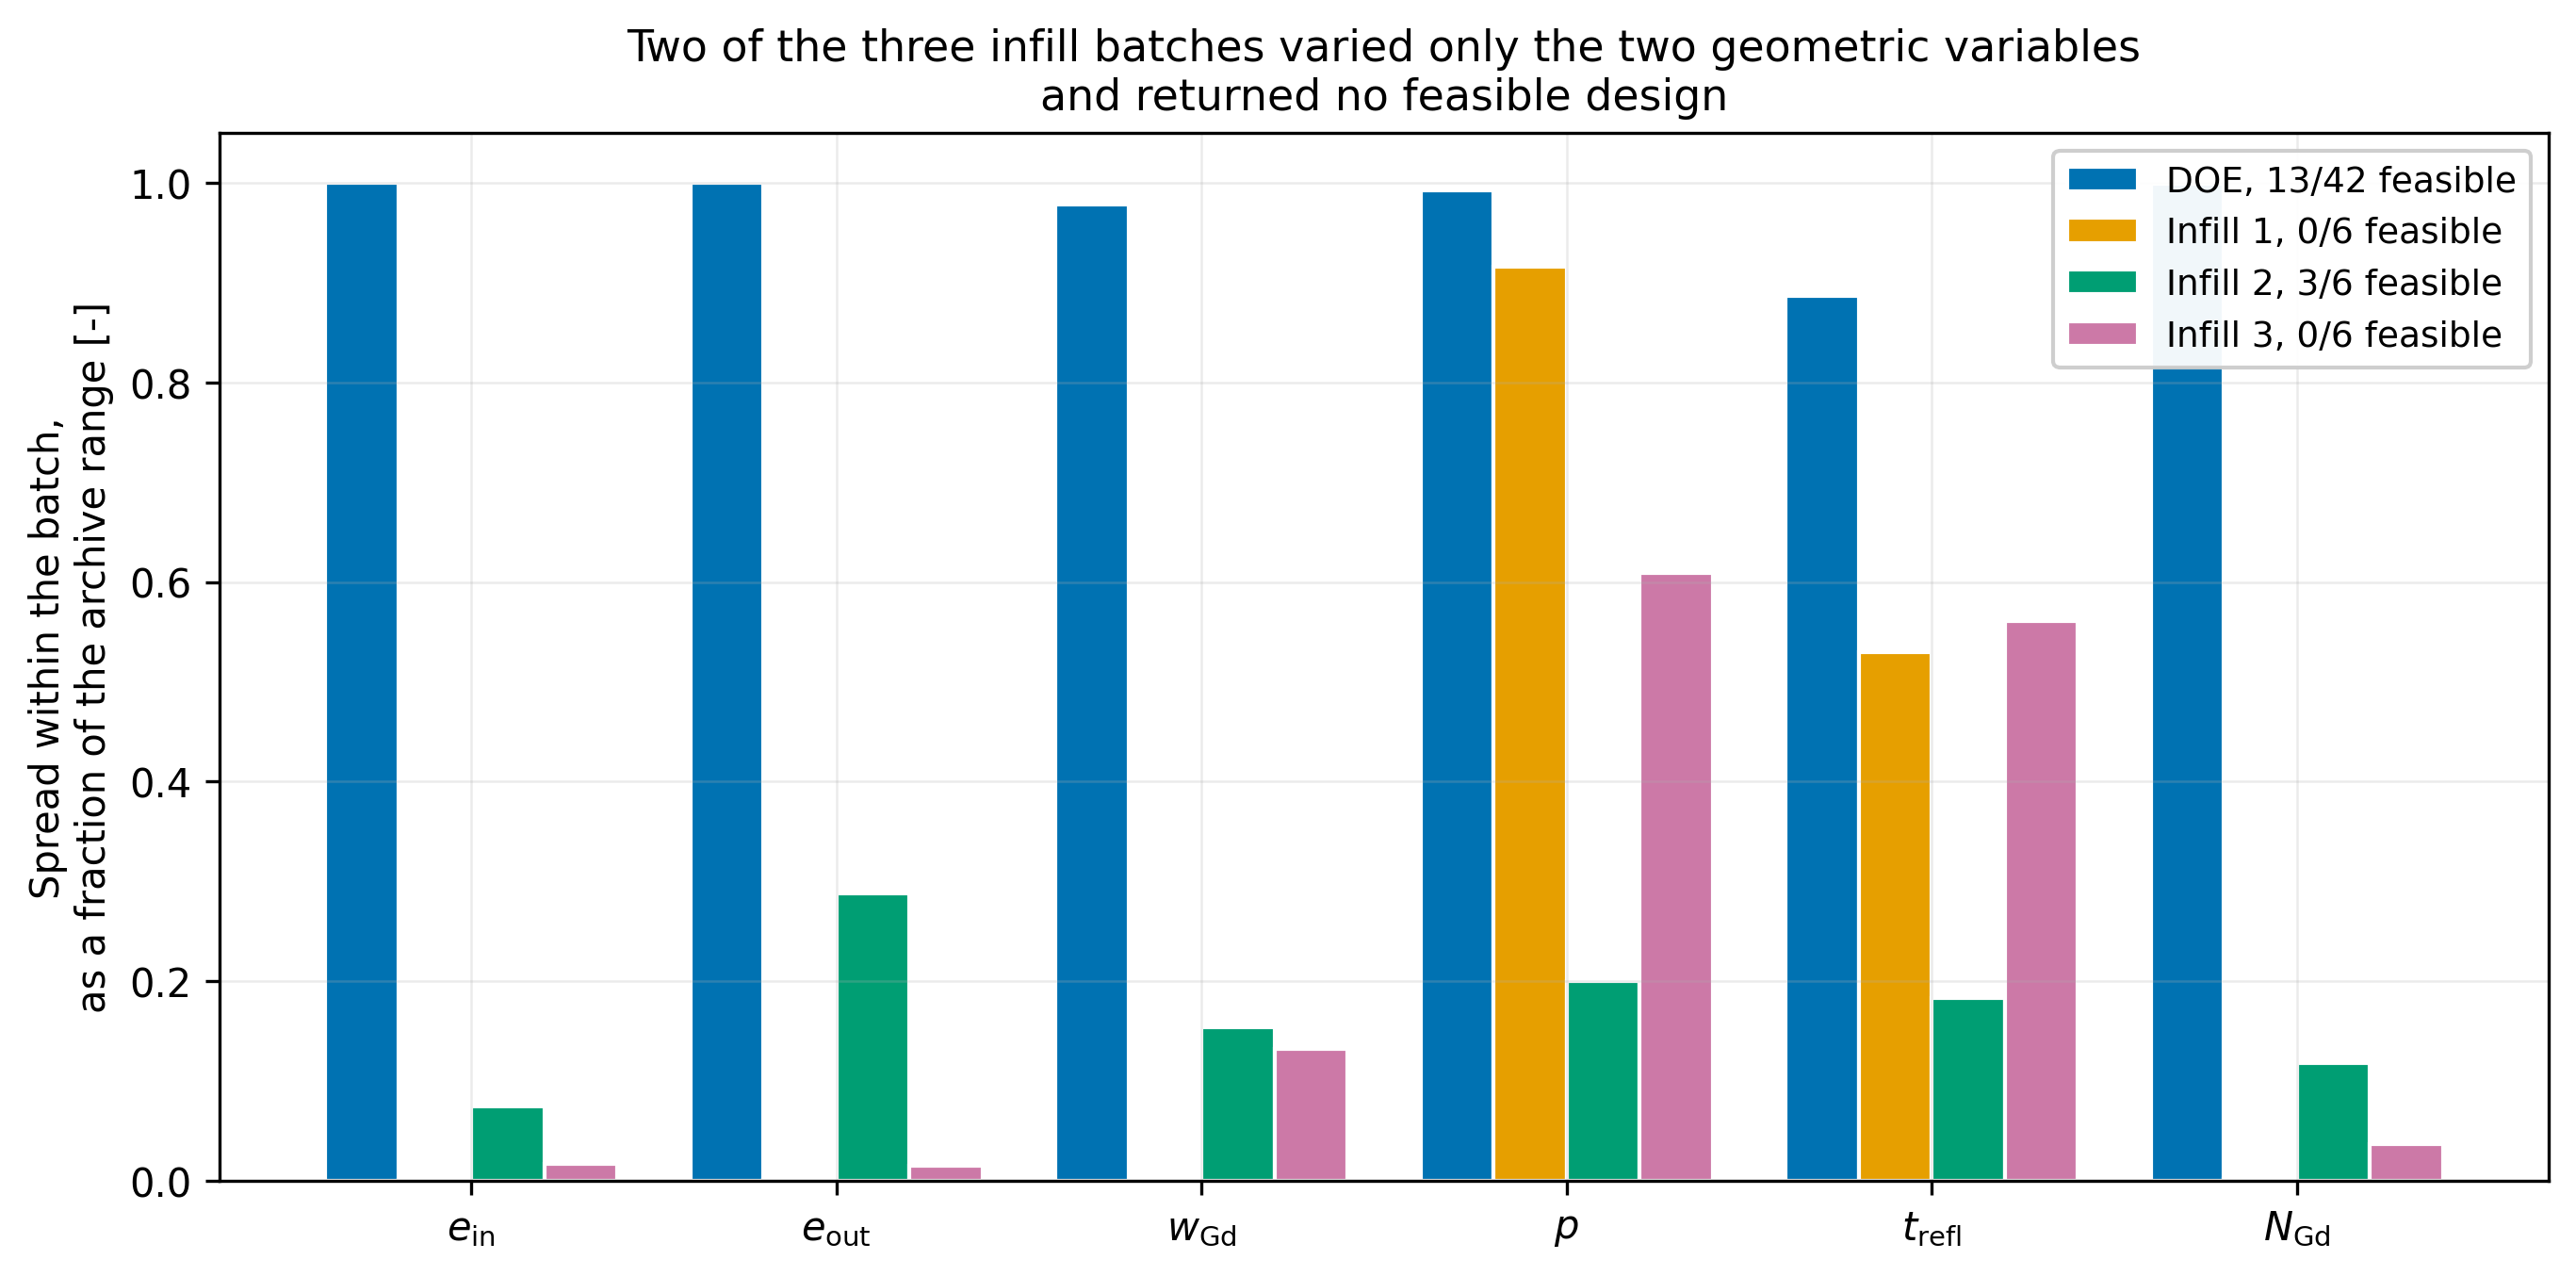
\includegraphics[width=\linewidth]{images/c7_infill_diversity}
  \caption{Within-block spread of each design variable, as a fraction
  of the archive range. Infill blocks 1 and 3 vary only the pitch and
  the reflector thickness, and neither returned a feasible design.}
  \label{fig:c7-diversity}
\end{figure}

Two of the three infill blocks collapsed. In block 1 the six designs
share one enrichment pair, \num{5.09} and \SI{4.04}{wt\%}, exactly zero
gadolinia and 24 poisoned pins, and differ only in pitch and reflector
thickness. In block 3 the same pattern recurs at \num{8.13} and
\SI{7.33}{wt\%} with 32 pins. All twelve designs of the two blocks
failed the reactivity ceiling.

The cause is a configuration regression, not a new defect. The
acquisition ran with a minimum separation of 0.05 and a feasibility
margin of 1.0 standard deviation, the default values of the launcher,
where Campaign 6 had established 0.14 and 1.5 in
Section~\ref{sec:res-c6-blocks}. The two collapsed blocks satisfied the
separation rule as coded, with pairwise separations of 0.059 to 0.089,
because the rule averages over all six variables and two of them
supplied the whole distance. A per-variable minimum spread would have
rejected both batches.

The consequence for the convergence record is that the flat
hypervolume of block 3 is not a stopping signal. Under the Campaign 6
rule a zero gain counts toward stopping only when the acquisition is
functioning, and block 3 demonstrably was not. The campaign therefore
ends with an unconverged front, and its value lies in the constraint
measurements rather than in the front itself.

\subsection{Feasibility and the nesting of the two screens}
\label{sec:res-c7-screens}

Of the 60 designs, 16 are feasible against all six constraints, a
fraction of \SI{26.7}{\%} against \SI{67}{\%} in the Campaign 6 design
of experiments. Table~\ref{tab:c7-nesting} gives the constraint census.
No design fails the enrichment or the geometric constraint, two fail
the peaking limit, nine fall below the reactivity floor, 34 exceed the
ceiling and 20 fail the controllability screen.

\begin{table}[htbp]
  \centering
  \caption{Constraint census of Campaign 7 and the joint activity of
  the two reactivity screens. Every design that fails the
  controllability screen also fails the derived ceiling, and fourteen
  designs fail the ceiling while passing the controllability screen.}
  \label{tab:c7-nesting}
  \begin{tabular}{lc}
    \toprule
    Outcome & Designs \\
    \midrule
    Fail $g_{k\max}$ at 1.126                      & 34 \\
    Fail $g_\mathrm{ctrl}$                         & 20 \\
    Fail $g_\mathrm{ctrl}$ and pass $g_{k\max}$    &  0 \\
    Fail $g_{k\max}$ and pass $g_\mathrm{ctrl}$    & 14 \\
    Pass every constraint except $g_{k\max}$       & 14 \\
    Feasible on all six                            & 16 \\
    \bottomrule
  \end{tabular}
\end{table}

\begin{figure}[htbp]
  \centering
  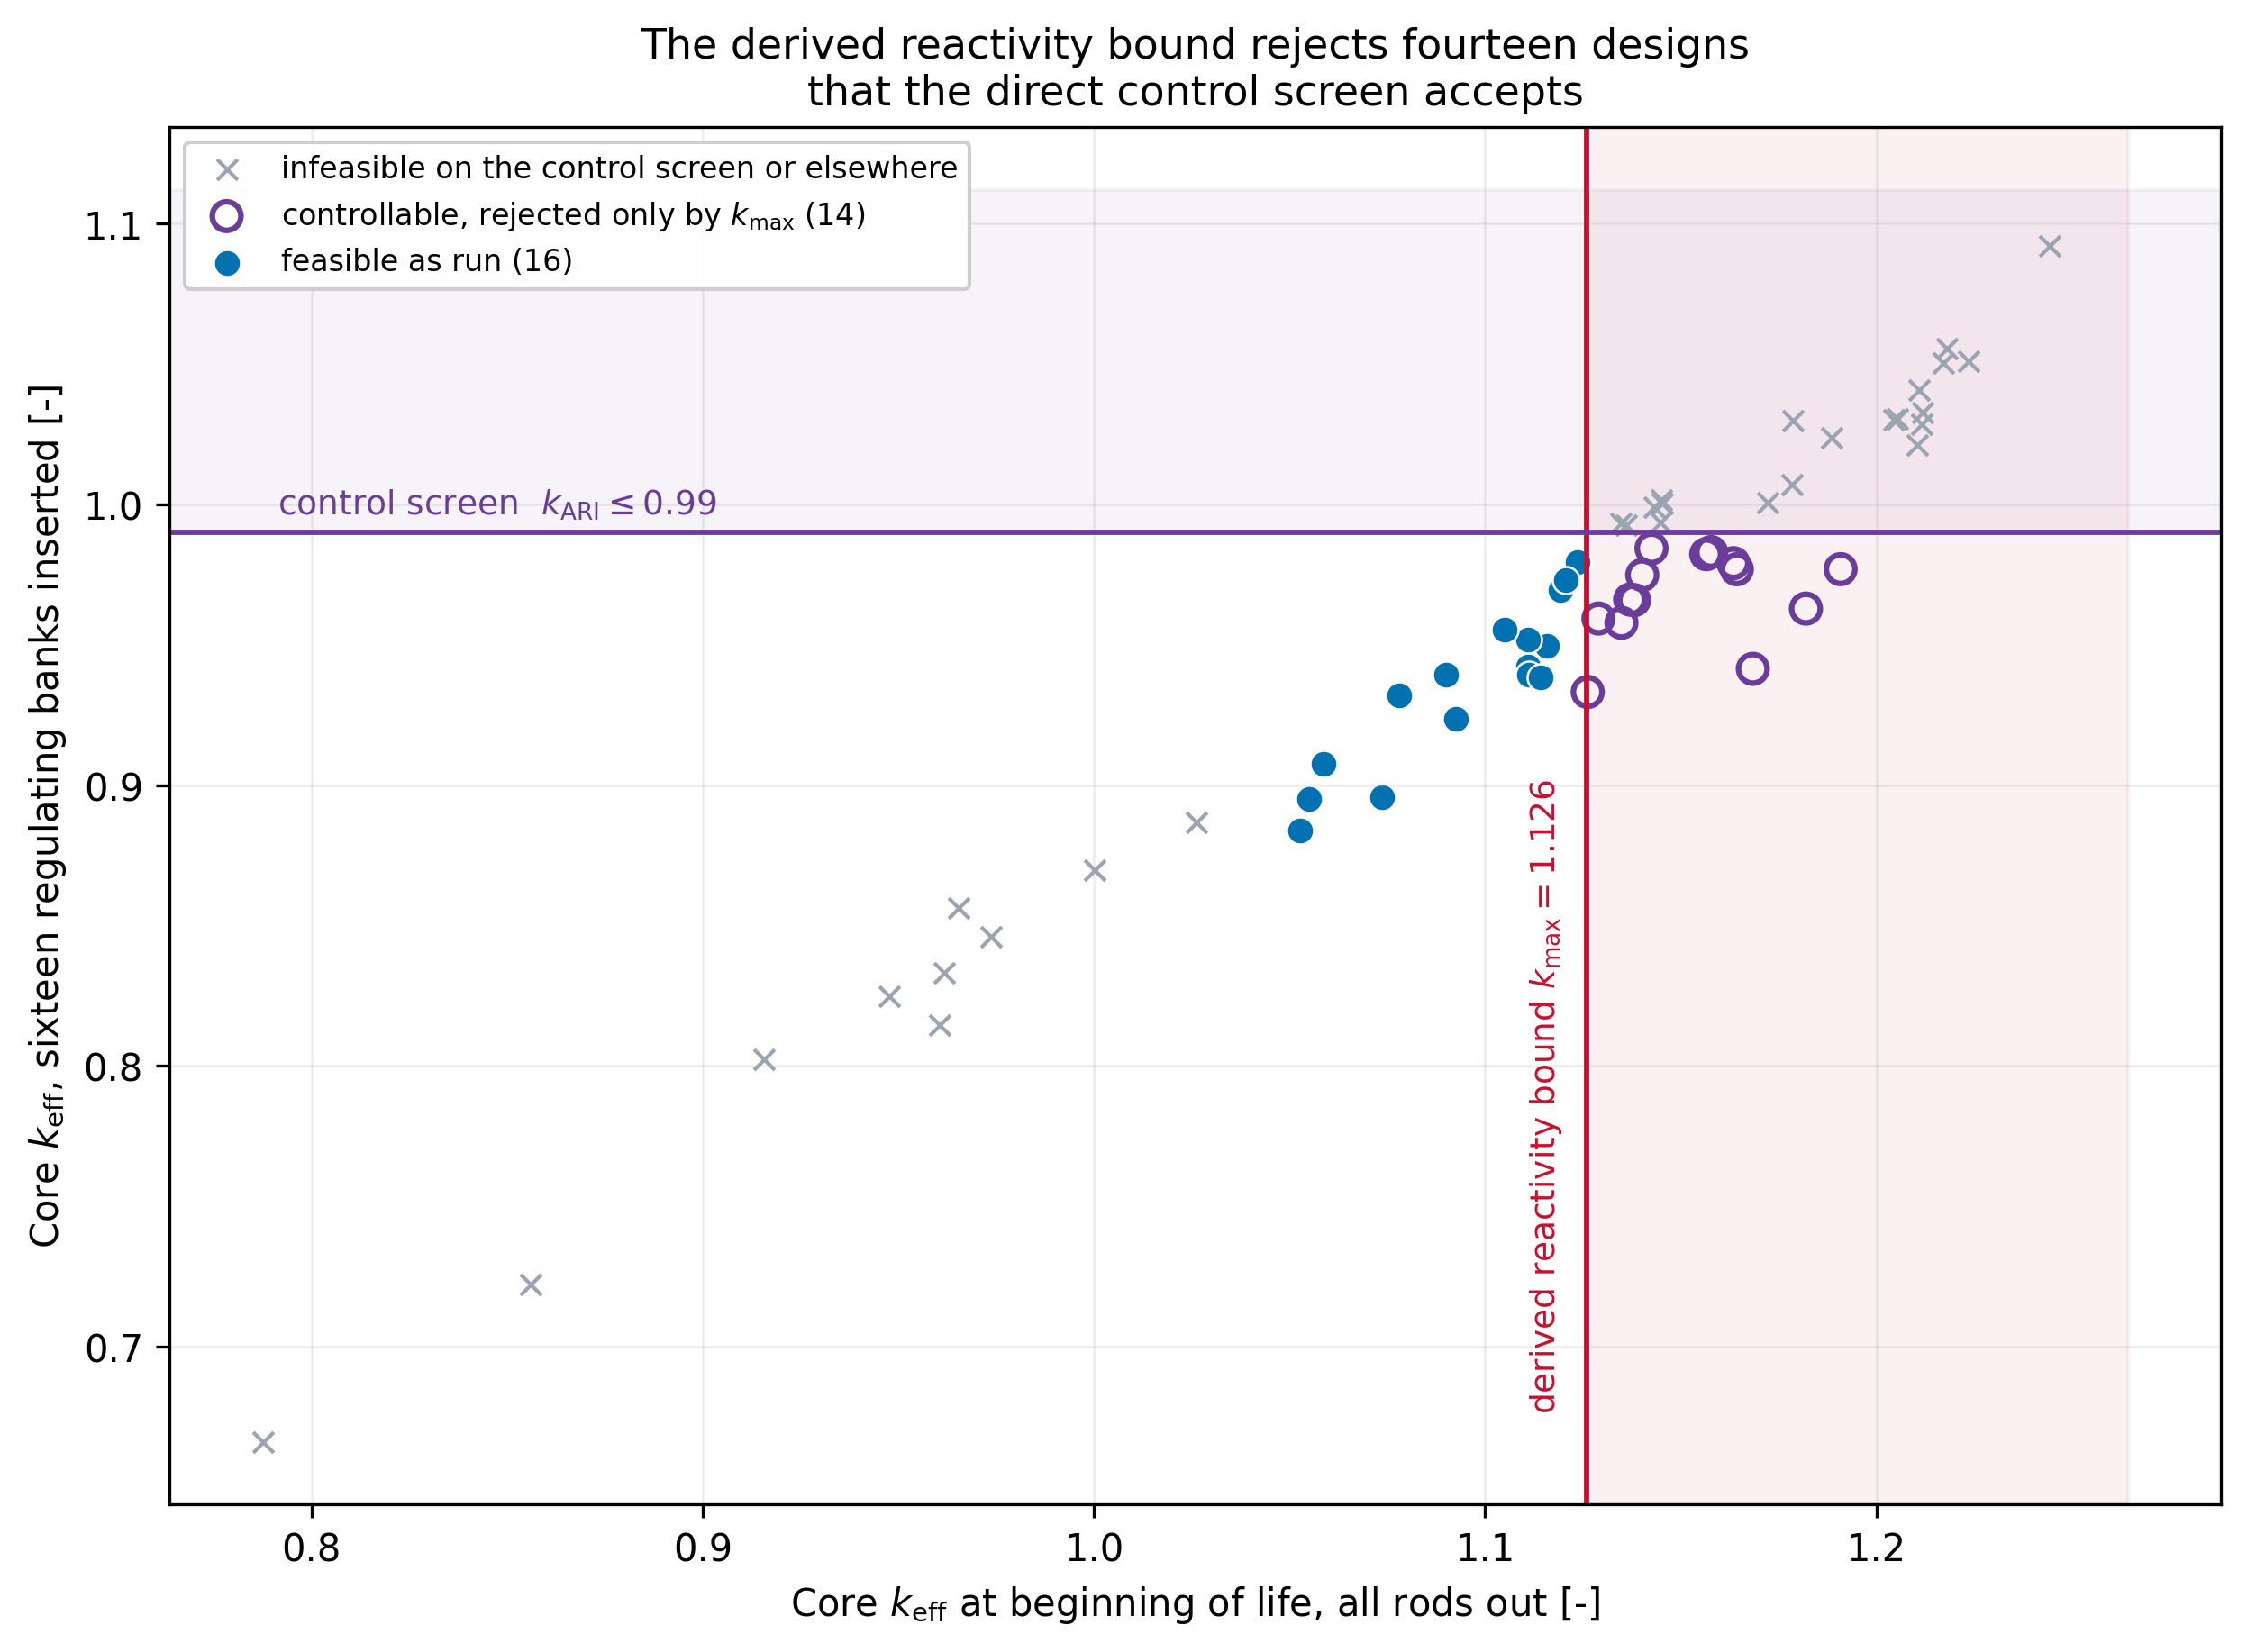
\includegraphics[width=0.9\linewidth]{images/c7_ctrl_screen}
  \caption{The two reactivity screens of Campaign 7 in the plane of
  the unrodded and the all-regulating-banks-in core eigenvalues. The
  derived ceiling at 1.126 rejects fourteen designs, marked by open
  circles, that the directly measured control screen accepts.}
  \label{fig:c7-screens}
\end{figure}

The two screens are nested. Not one design in the archive fails the
control screen without also failing the derived ceiling, and fourteen
designs fail the ceiling while their own measured bank worth shows them
controllable at the stated margin. Figure~\ref{fig:c7-screens} shows
the nesting directly. The ceiling of 1.126 therefore did no work that
the measurement did not do, and it discarded fourteen evaluations that
the measurement would have kept.

The derivation explains why. The eight Campaign 6 designs from which
1.126 was obtained had worths between \num{12174} and
\SI{12718}{pcm}, a spread of four per cent. The 60 designs of this
campaign span \num{10936} to \SI{22699}{pcm}, a factor of two. Eight
near-identical designs under-sampled the variability by an order of
magnitude, and the resulting bound is at once too tight where it
matters and not conservative in general. Restricted to the 22 designs
with an unrodded eigenvalue between 1.09 and 1.17, the smallest
measured worth of \SI{14126}{pcm} implies a ceiling of 1.151, while the
smallest worth in the whole archive implies 1.110.

The front reflects the same fact. As run, the feasible non-dominated set
holds three designs, all from infill block 2. With the derived ceiling
removed and the measured control screen retained, the feasible set grows
from 16 to 30 designs, the front doubles to six, the peaking floor moves
from 1.565 to 1.525, and the hypervolume against the frozen reference
rises from 996.5 to 1054.1, a gain of \SI{5.8}{\%}. Three of the six
designs come from infill block 3, the block that under the ceiling
contributed nothing. Table~\ref{tab:c7-front} lists both fronts and
Figure~\ref{fig:c7-pareto} places them in the objective plane.

\begin{table}[htbp]
  \centering
  \small
  \caption{The Campaign 7 front under the two screening rules. Designs
  48, 53 and 49 form the front as run. All six form the front when the
  measured control screen alone governs reactivity. Bank worth is the
  difference between the unrodded and the all-banks-in eigenvalues.}
  \label{tab:c7-front}
  \begin{tabular}{ccccccccccc}
    \toprule
    Design & EFPD & $F_{\Delta H}$ & $e_\mathrm{in}$ & $e_\mathrm{out}$ & $w_\mathrm{Gd}$ & $p$ & $t_\mathrm{refl}$ & $n_\mathrm{Gd}$ & $k_\mathrm{eff}^\mathrm{core}$ & worth \\
           & [d] & [-] & [wt\%] & [wt\%] & [wt\%] & [cm] & [cm] & [-] & [-] & [pcm] \\
    \midrule
    59 & 3886 & 1.525 & 8.13 & 7.33 & 1.10 & 1.150 & 19.49 & 32 & 1.135 & 17699 \\
    57 & 4045 & 1.528 & 8.13 & 7.33 & 1.21 & 1.176 & 17.87 & 32 & 1.137 & 17094 \\
    55 & 4502 & 1.529 & 8.14 & 7.34 & 1.10 & 1.238 & 14.09 & 32 & 1.143 & 15815 \\
    48 & 4745 & 1.565 & 8.71 & 7.80 & 1.93 & 1.237 & 14.06 & 40 & 1.119 & 14970 \\
    53 & 4899 & 1.590 & 8.97 & 7.88 & 1.96 & 1.249 & 13.21 & 40 & 1.121 & 14734 \\
    49 & 5087 & 1.598 & 9.19 & 8.30 & 2.13 & 1.267 & 12.29 & 40 & 1.124 & 14416 \\
    \bottomrule
  \end{tabular}
\end{table}

\begin{figure}[htbp]
  \centering
  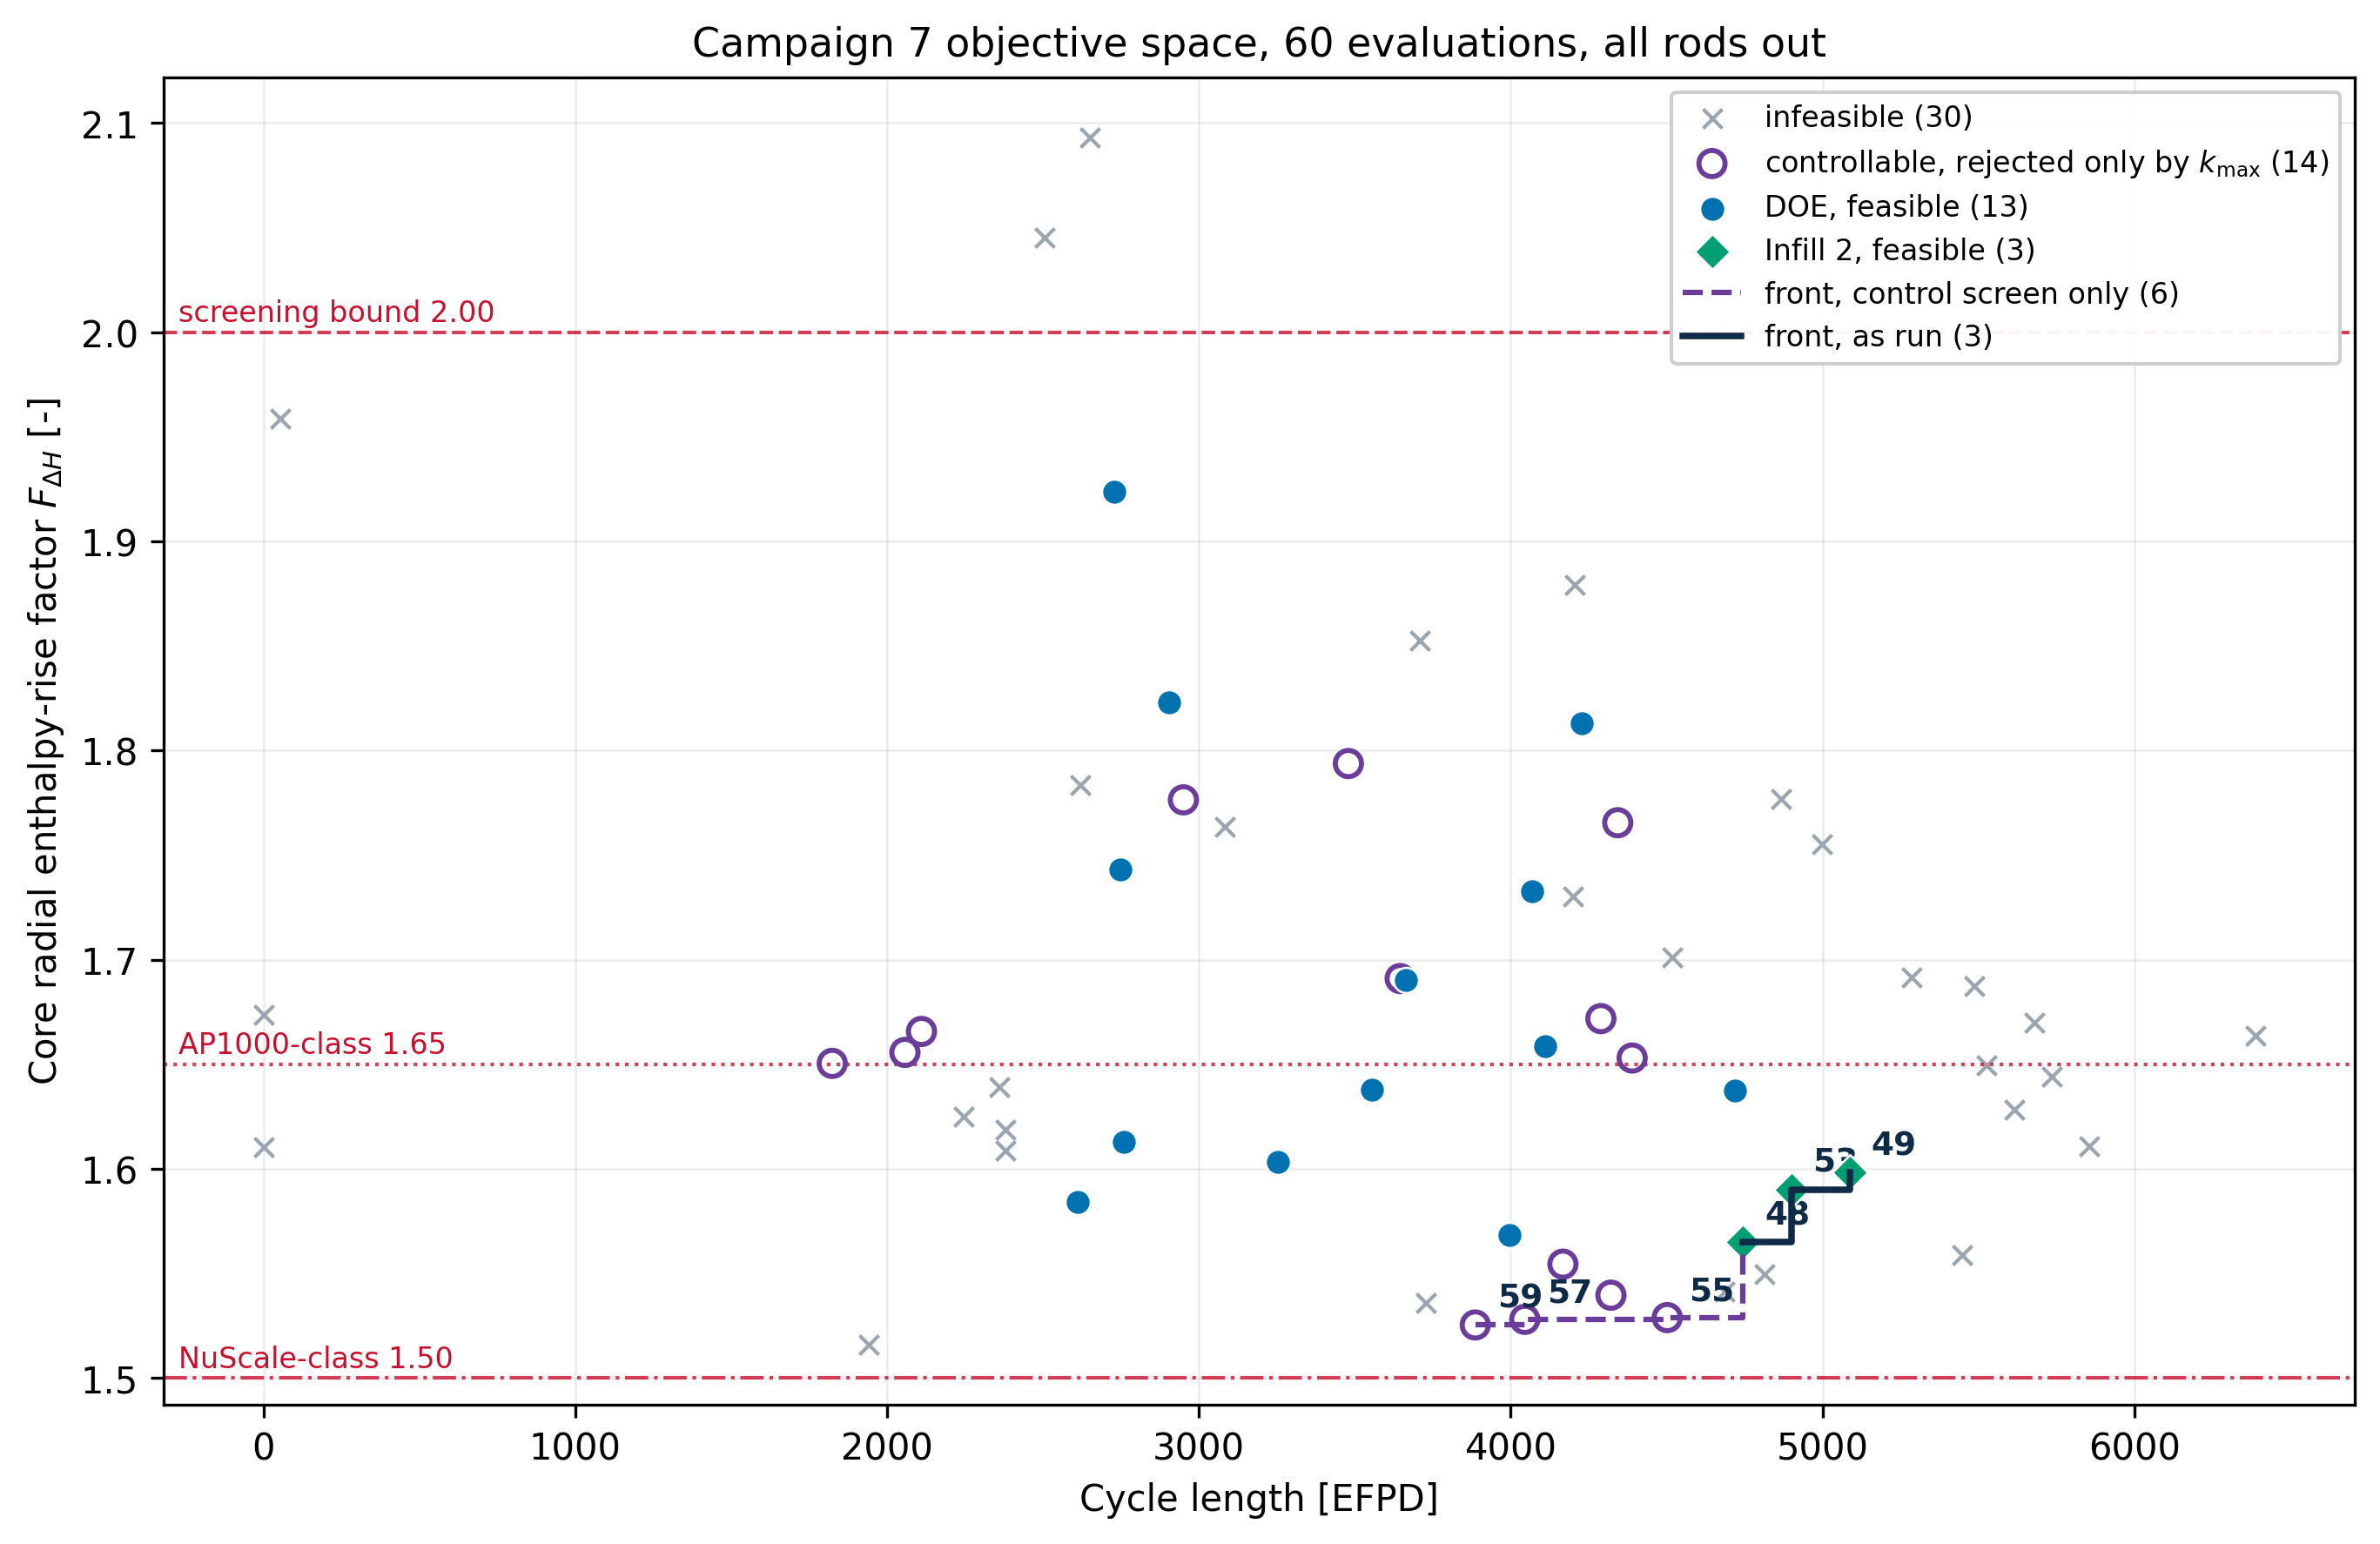
\includegraphics[width=\linewidth]{images/c7_pareto_60}
  \caption{Campaign 7 objective space with all rods out. Filled markers
  are feasible as run, open circles are controllable designs rejected
  only by the derived ceiling. The solid front is the one the campaign
  reported and the dashed front is the one the measured control screen
  supports.}
  \label{fig:c7-pareto}
\end{figure}

Two properties of the front as run deserve stating. Its three designs
sit \num{240} to \SI{680}{pcm} below the ceiling, so the front is a
constraint boundary and not an interior trade. And the cycle lengths
are not comparable with Campaign 6, because the enrichment box is a
different one, and the longest feasible cycle of 5087 EFPD says nothing
about the reactor class that the 9981 EFPD of Campaign 6 did not
already say.

%% AUTHOR: one paragraph on why the low-peaking end of the control-screen
%% front lives at thick reflectors and narrow pitch, and on the physical
%% meaning of a front that doubles when a surrogate bound is removed.

\subsection{Regulating-bank worth and the reason the screens nest}
\label{sec:res-c7-worth}

The worth of the sixteen regulating banks is defined on the two core
solves of every evaluation.

\begin{equation}
\rho_\mathrm{bank}(\mathbf{x}) = k_\mathrm{eff}^\mathrm{core}(\mathbf{x}) - k_\mathrm{ARI}(\mathbf{x})
\label{eq:bank-worth}
\end{equation}

\noindent where the symbols have the following meaning.

\begin{itemize}
  \item $\rho_\mathrm{bank}$ is the bank worth in units of $k$,
        dimensionless, reported in pcm by multiplying by $10^5$.

  \item $k_\mathrm{eff}^\mathrm{core}$ is the unrodded core eigenvalue
        at beginning of life, dimensionless.

  \item $k_\mathrm{ARI}$ is the eigenvalue with all sixteen regulating
        banks inserted, dimensionless.
\end{itemize}

Across the archive the worth ranges from \num{10936} to
\SI{22699}{pcm} with a median of \SI{16510}{pcm}. Figure~\ref{fig:c7-worth}
shows its two strongest drivers and Figure~\ref{fig:c7-influence} the
rank correlations of all six variables with the objectives, the worth
and the rodded peaking.

\begin{figure}[htbp]
  \centering
  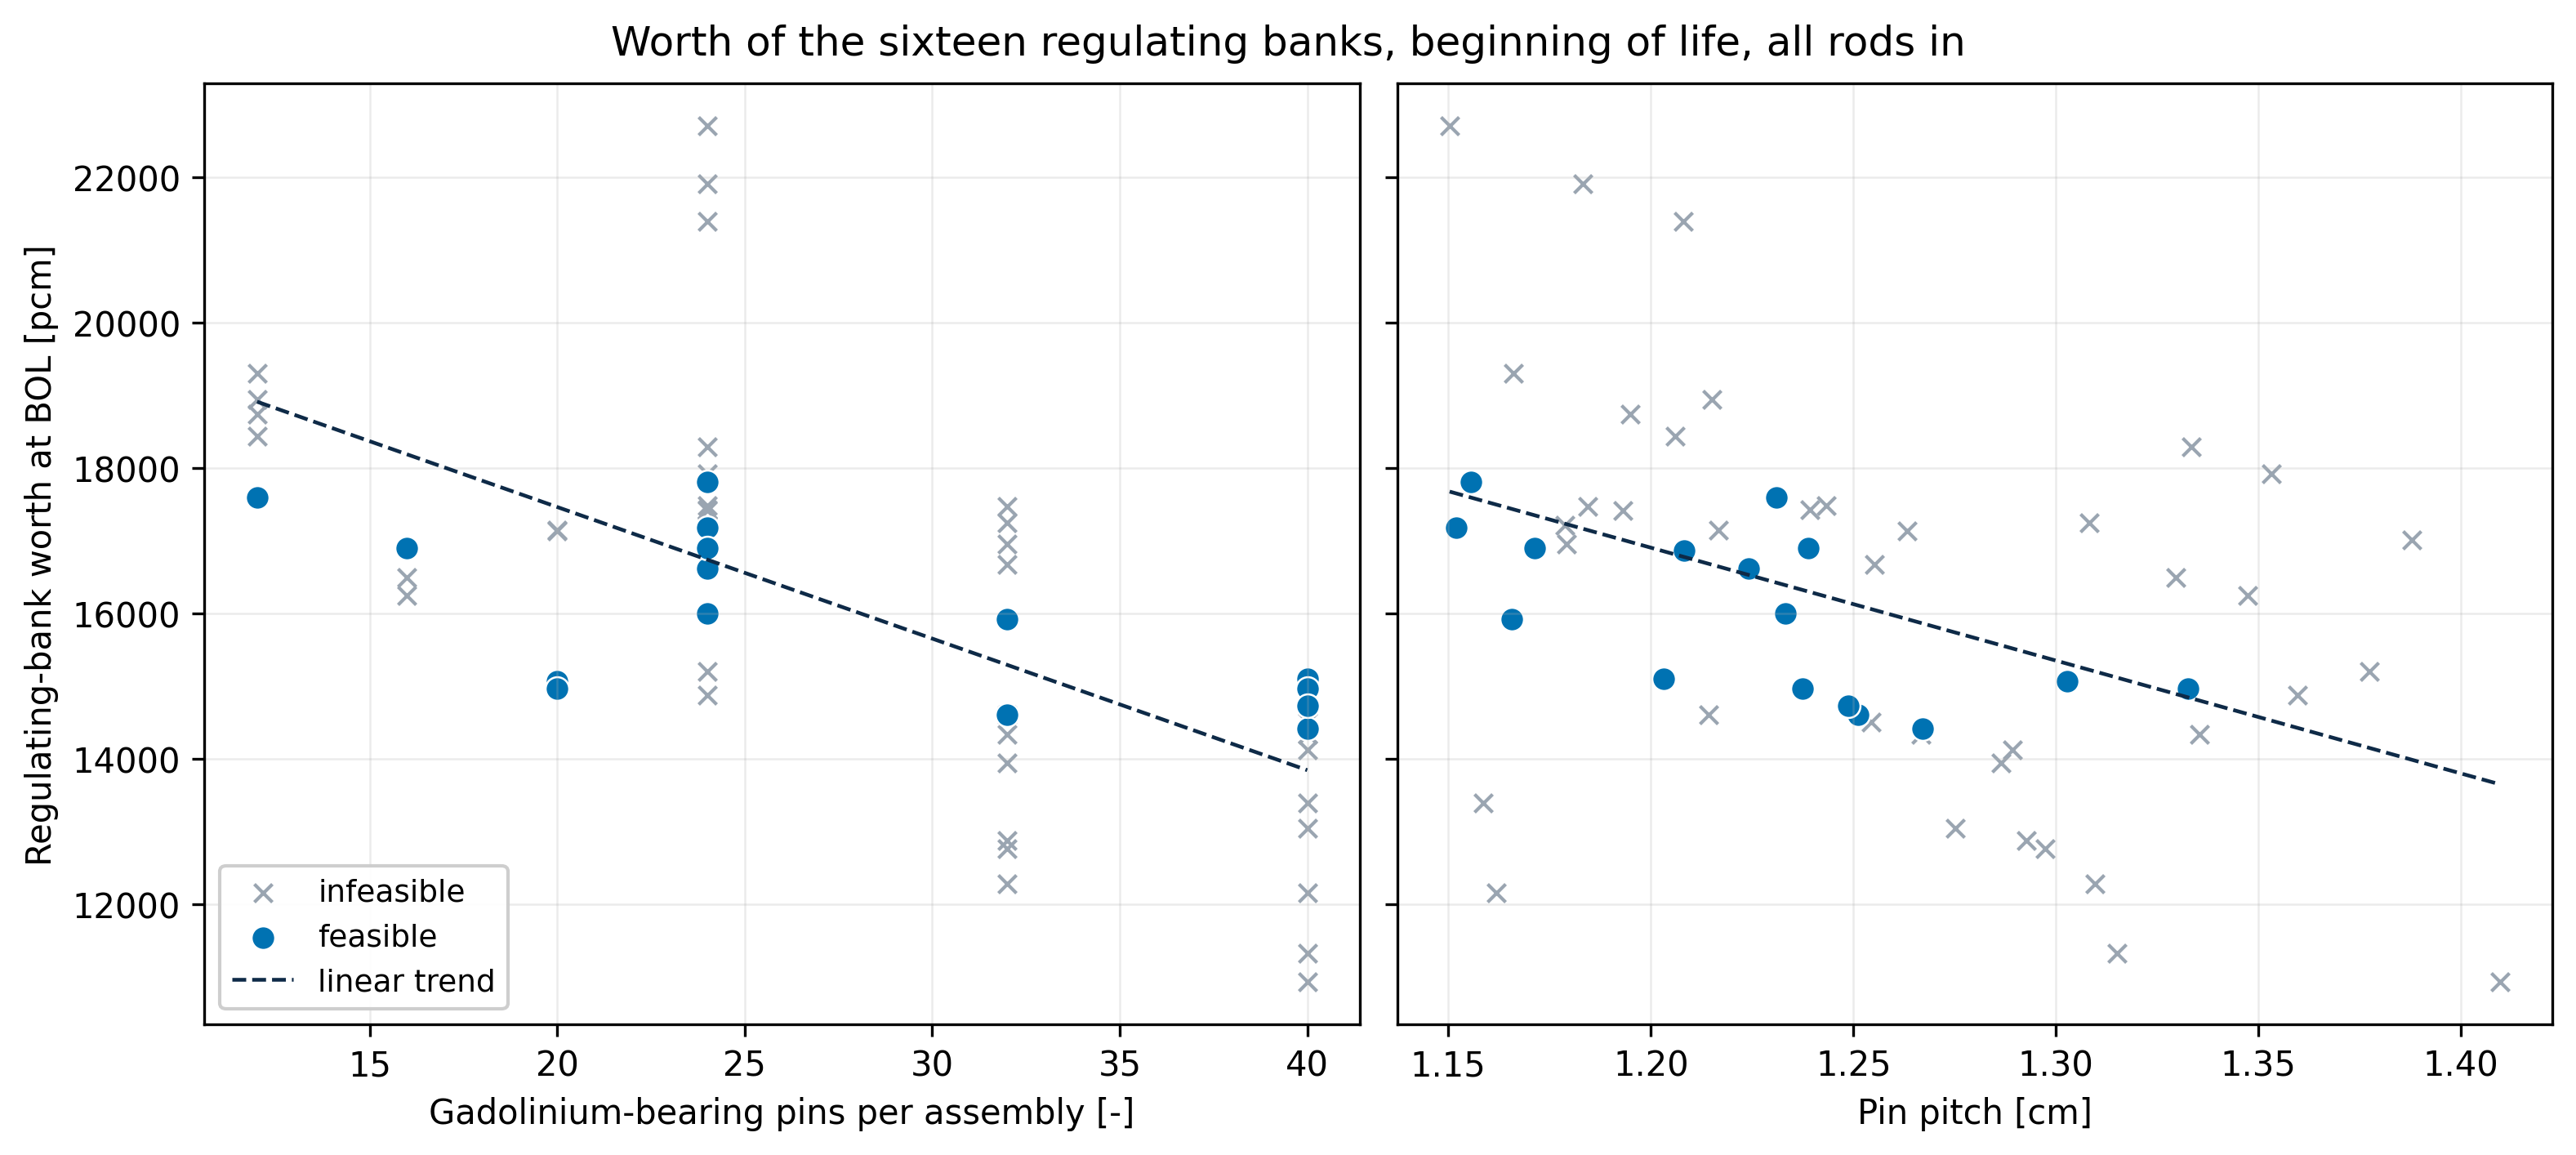
\includegraphics[width=\linewidth]{images/c7_rod_worth}
  \caption{Worth of the sixteen regulating banks against the
  gadolinium pin count and the pin pitch. The dashed lines are
  least-squares trends and serve only as visual guides.}
  \label{fig:c7-worth}
\end{figure}

\begin{figure}[htbp]
  \centering
  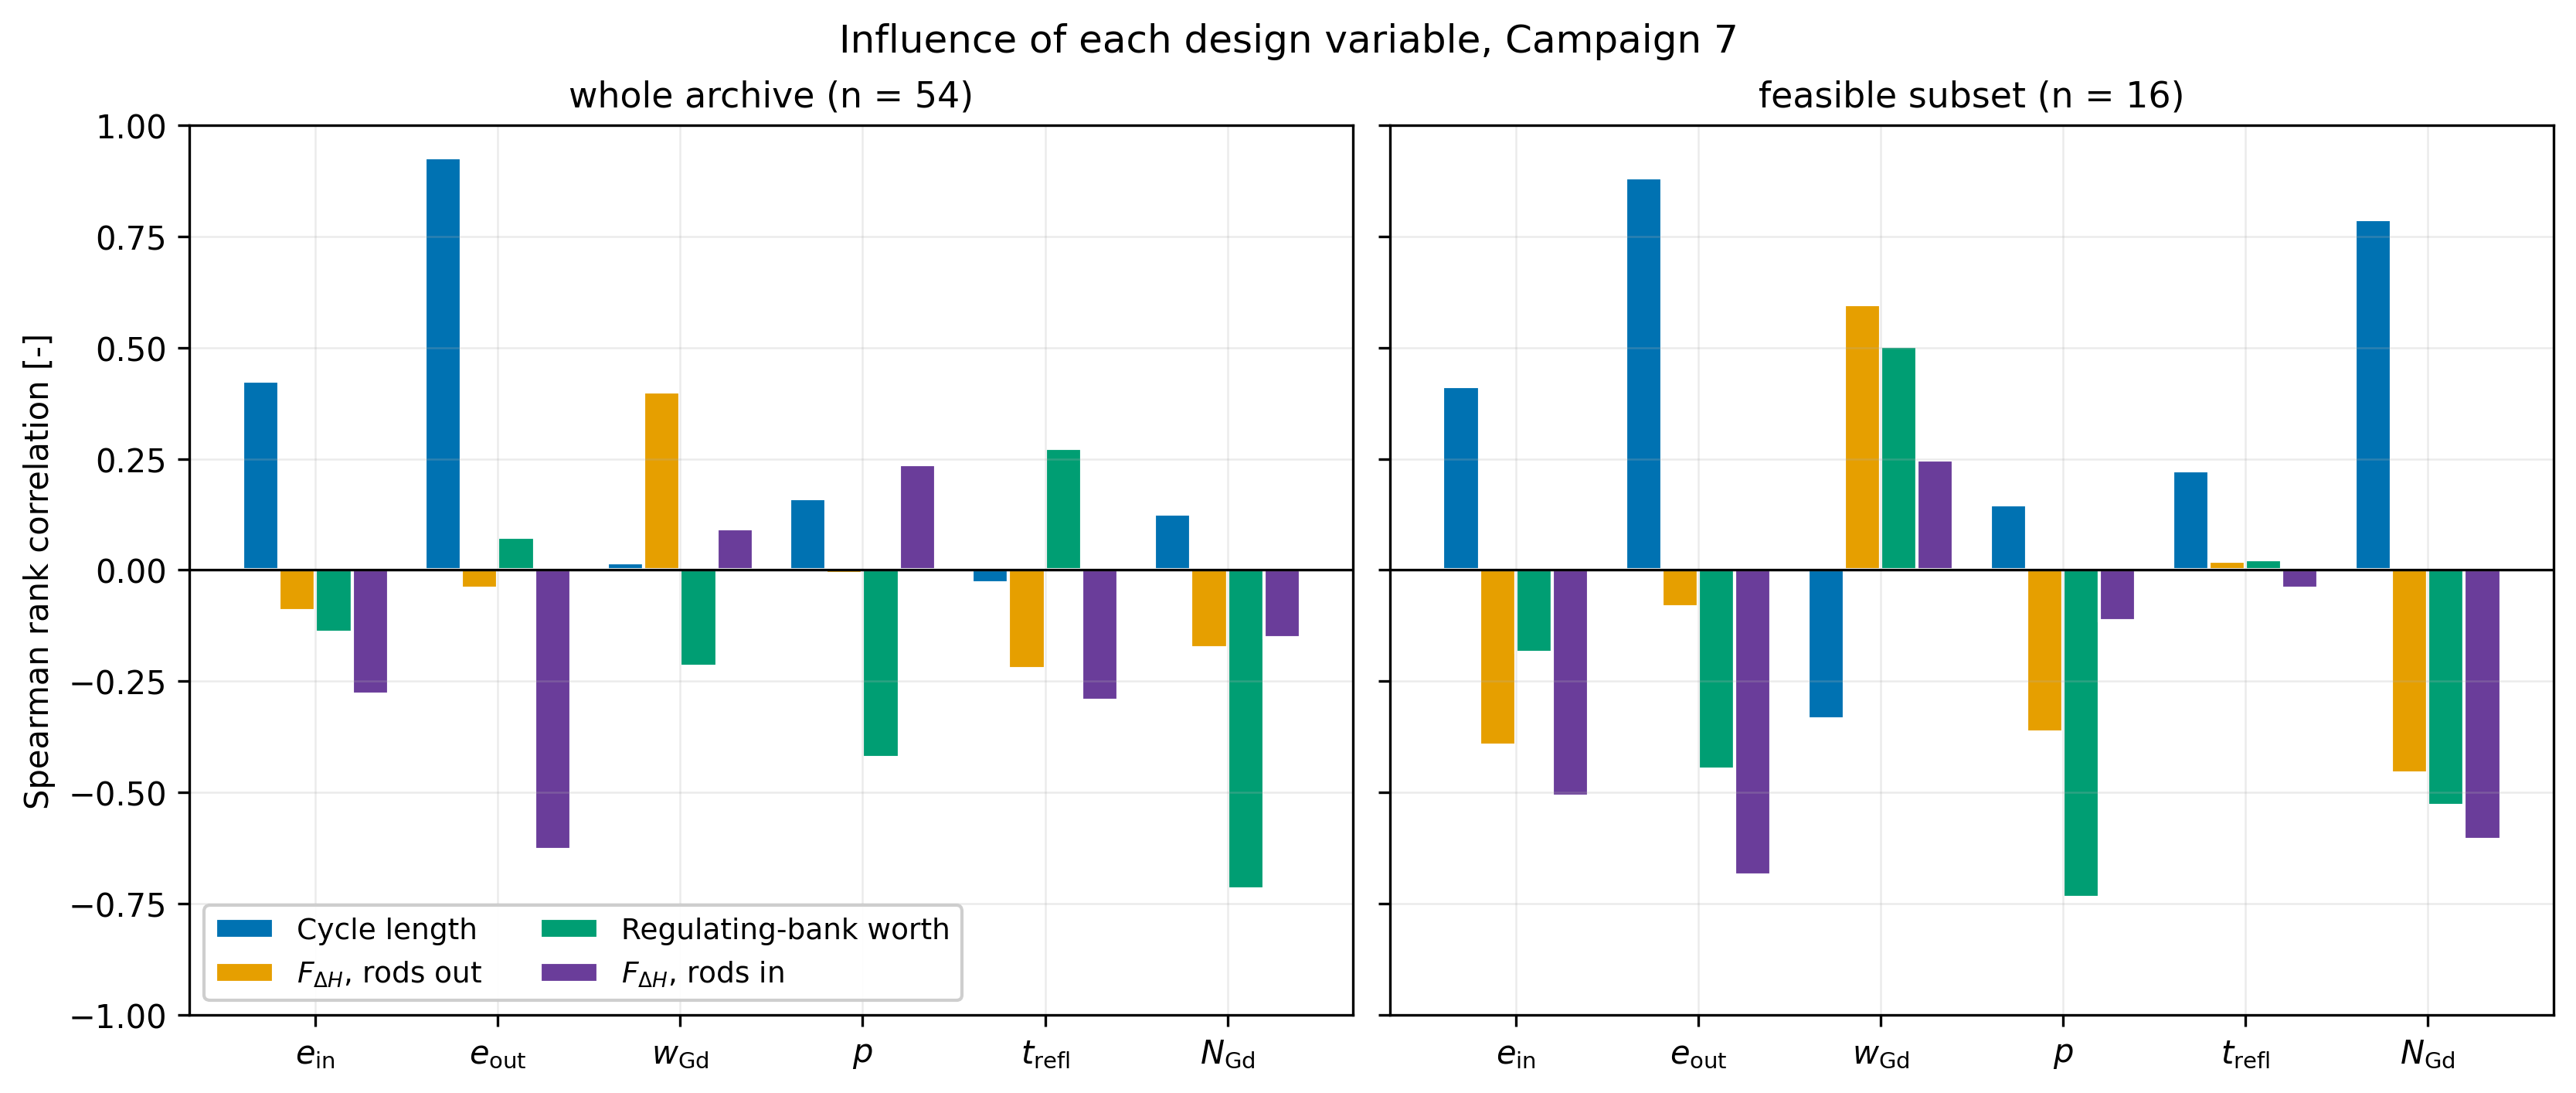
\includegraphics[width=\linewidth]{images/c7_vars_influence}
  \caption{Spearman rank correlation of each design variable with the
  two objectives, the regulating-bank worth and the peaking with the
  banks inserted, over the whole archive and over the feasible subset.}
  \label{fig:c7-influence}
\end{figure}

The worth correlates at $-0.68$ with the gadolinium pin count, at
$-0.45$ with the pitch and at $+0.61$ with the unrodded eigenvalue.
Gadolinium depresses the eigenvalue and the bank worth together, so the
designs with the least worth are the heavily poisoned ones, which are
already far below the ceiling for a different reason. That is why the
two screens nest in this design space, and it is also why the
eight-design derivation of the ceiling looked safe when it was not.
The eight designs were all high-enrichment, forty-pin designs from one
corner of the Campaign 6 front, and their worths were alike because
their poison inventories were alike.

The measurement also settles a question left open since Campaign 4.
The ceiling of 1.35 used in Campaigns 1 to 6 was described as a
screening value not traceable to a primary source. Deriving the
ceiling from the worth of all seven banks, that is all 32 control rod
assemblies, with the same \SI{1000}{pcm} margin gives 1.368. The value
used through six campaigns sits two per cent below the measured
all-bank controllability bound of this core. It is a measured quantity
in retrospect, and the methodology chapter now states it as such,
with the caveat that an all-bank insertion with a \SI{1000}{pcm}
operating margin is not a licensing shutdown margin, which also
requires the highest-worth assembly stuck out and the cold, xenon-free
state.

\subsection{Peaking with the regulating banks inserted}
\label{sec:res-c7-rodded}

The peaking objective is evaluated with all rods out. The same core
solve that measures $k_\mathrm{ARI}$ also yields the radial peaking
with the sixteen banks inserted, and Figure~\ref{fig:c7-rodded} plots
the two against each other.

\begin{figure}[htbp]
  \centering
  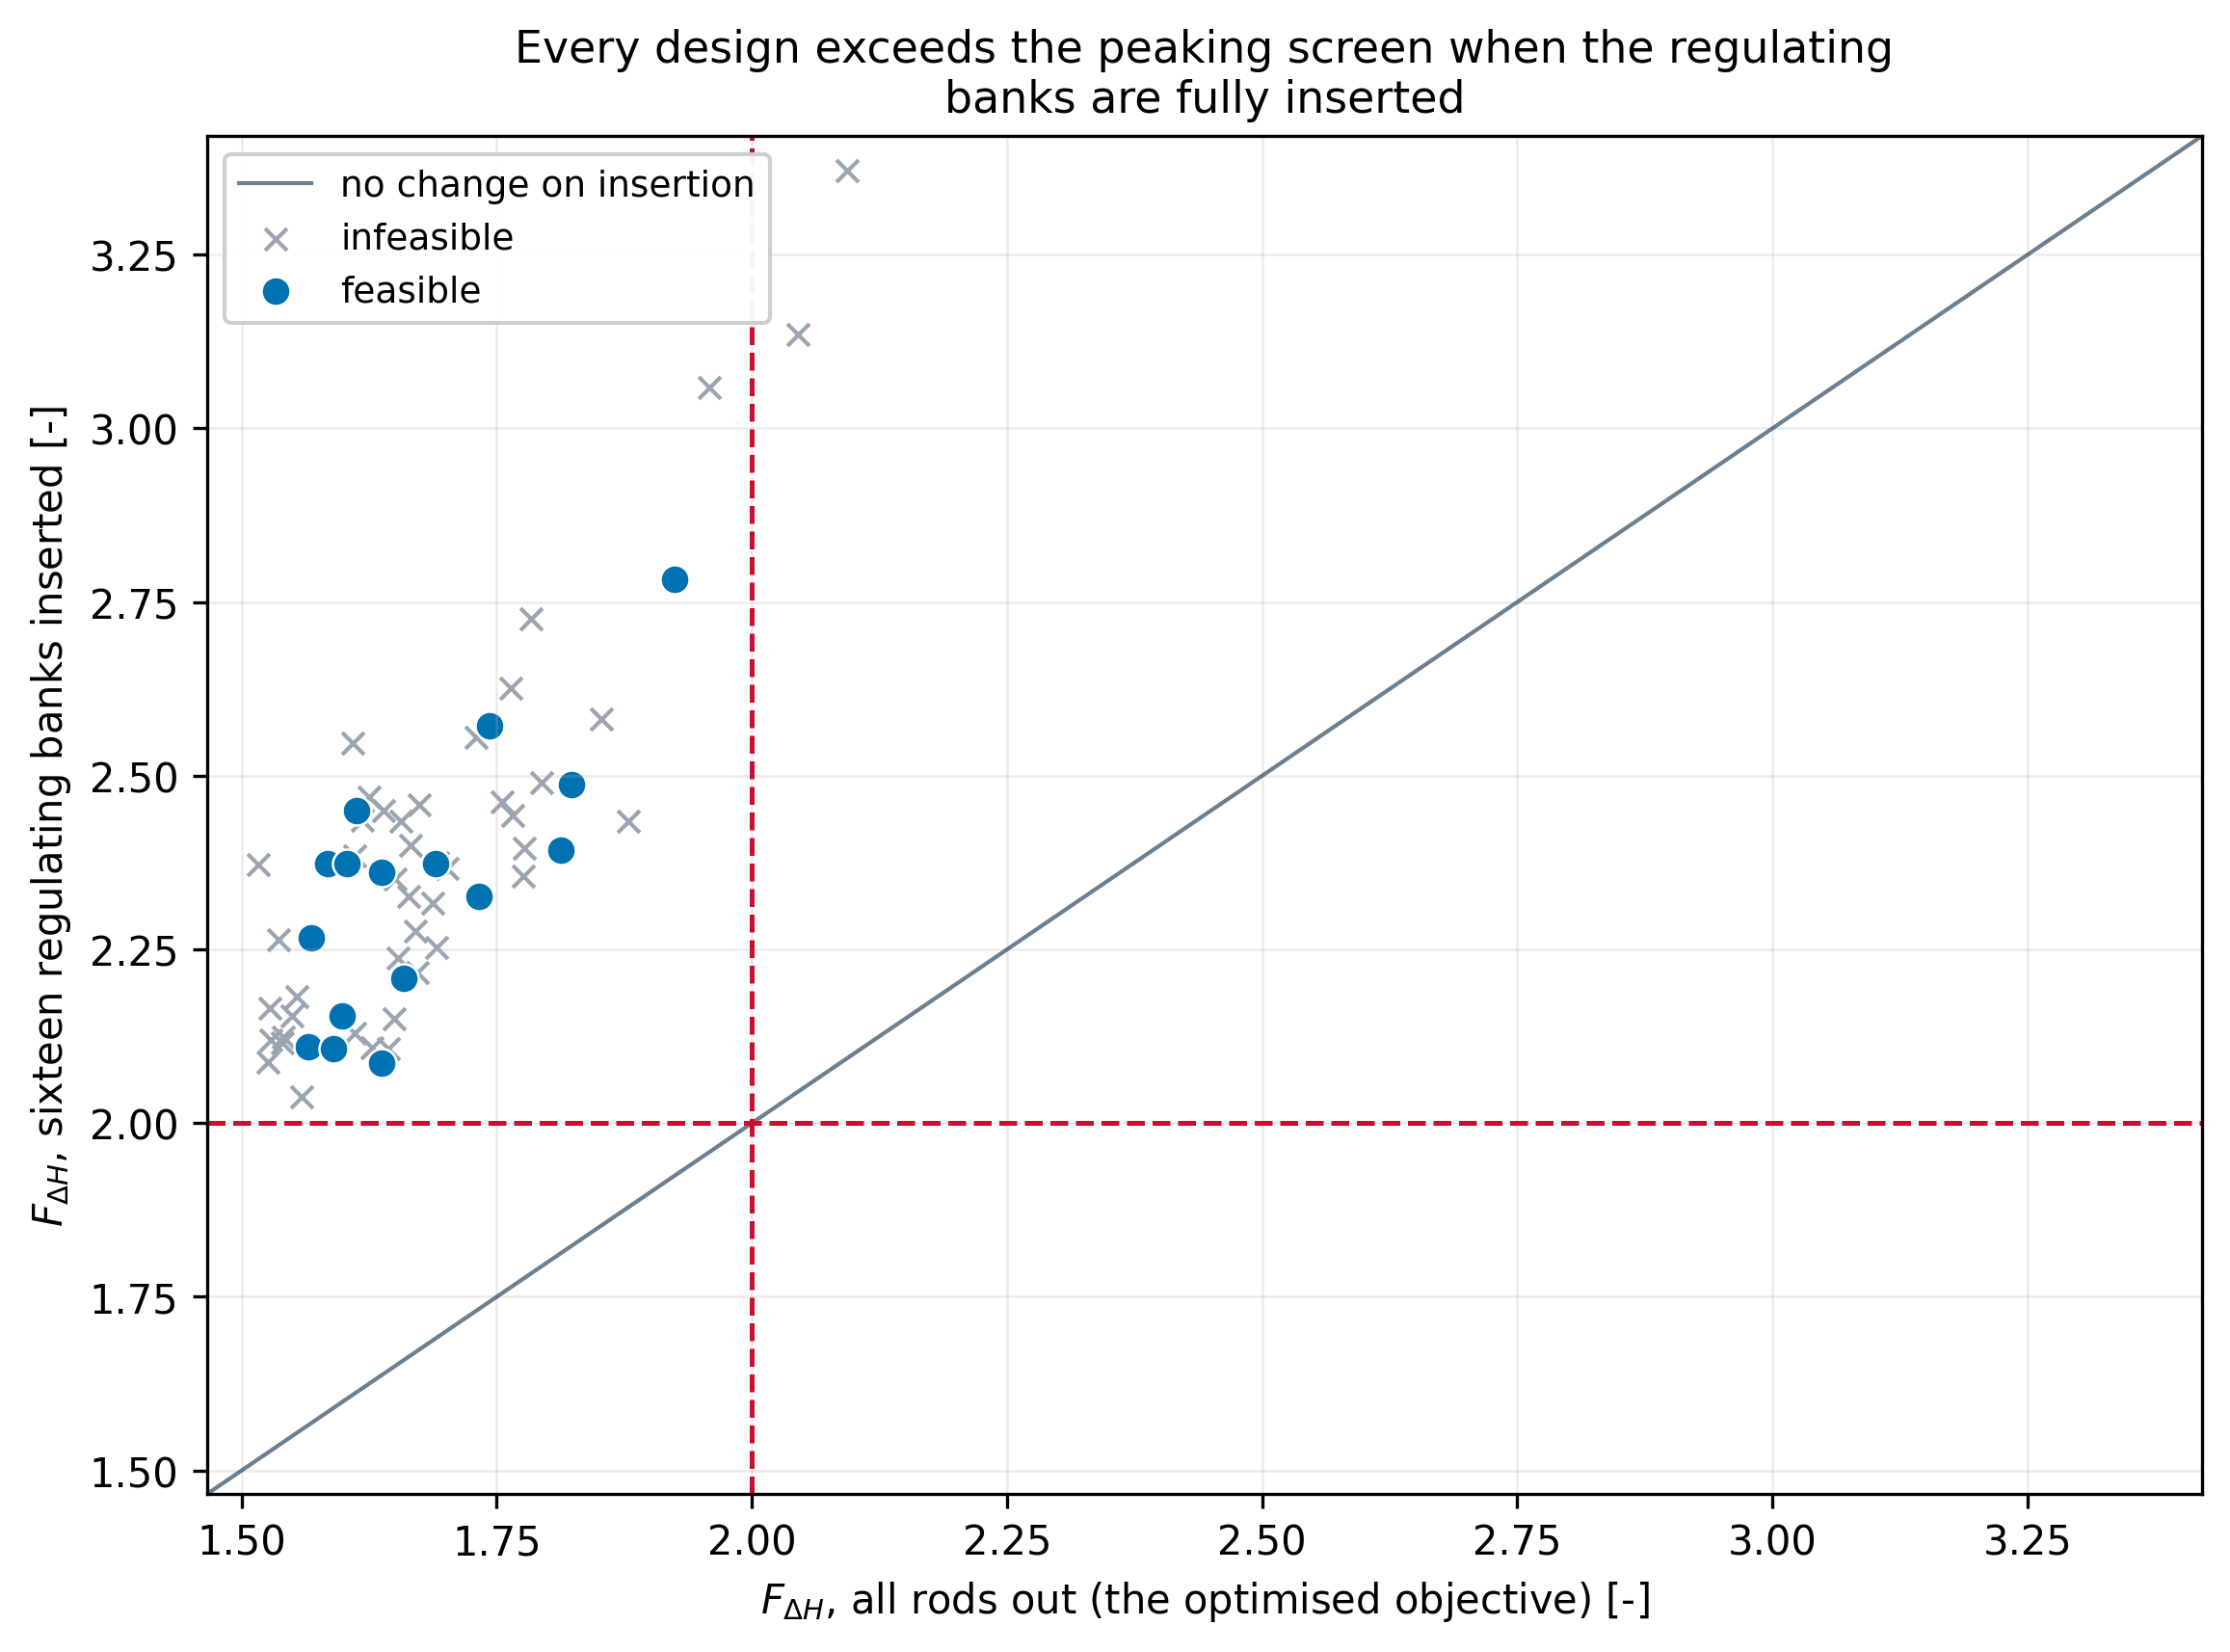
\includegraphics[width=0.85\linewidth]{images/c7_rodded_peaking}
  \caption{Radial peaking with all rods out, the optimised objective,
  against the same quantity with the sixteen regulating banks inserted.
  Every design lies above the screening bound of 2.0 in the rodded
  configuration.}
  \label{fig:c7-rodded}
\end{figure}

With the banks inserted $F_{\Delta H}$ runs from 2.038 to 3.371 with a
mean of 2.375, against 1.516 to 2.093 unrodded. The insertion penalty
ranges from 0.449 to 1.278 and is design dependent, correlating at
$-0.81$ with the outer-zone enrichment over the archive. Every one of
the 60 designs exceeds the screening bound of 2.0 in the rodded
configuration, and the three front designs sit between 2.11 and 2.16.

Two framings are required and neither should be overstated. Sixteen
banks fully inserted is the extreme of the regulating band used here as
a controllability test, not an operating configuration, so the rodded
value is an upper bound on operating peaking rather than an operating
value. Even so, the objective being minimised moves by half a unit or
more when the rods go in, and it moves by a design-dependent amount.
A design selected for low unrodded peaking is not thereby a design
with low rodded peaking. This is recorded as a limitation of the
objective set and as the motivation for the two-level reading of
Campaign 8.

%% AUTHOR: physical interpretation of the negative correlation between
%% the insertion penalty and the outer-zone enrichment.

\subsection{Depletion histories and the statistical error on the cycle length}
\label{sec:res-c7-uncertainty}

The assembly depletion solves are the only transport runs whose output
reaches the campaign log, and the log therefore holds the complete
$k_\infty(B)$ history of every design. Figure~\ref{fig:c7-histories}
reconstructs all 60 histories with the end-of-cycle crossing marked.

\begin{figure}[htbp]
  \centering
  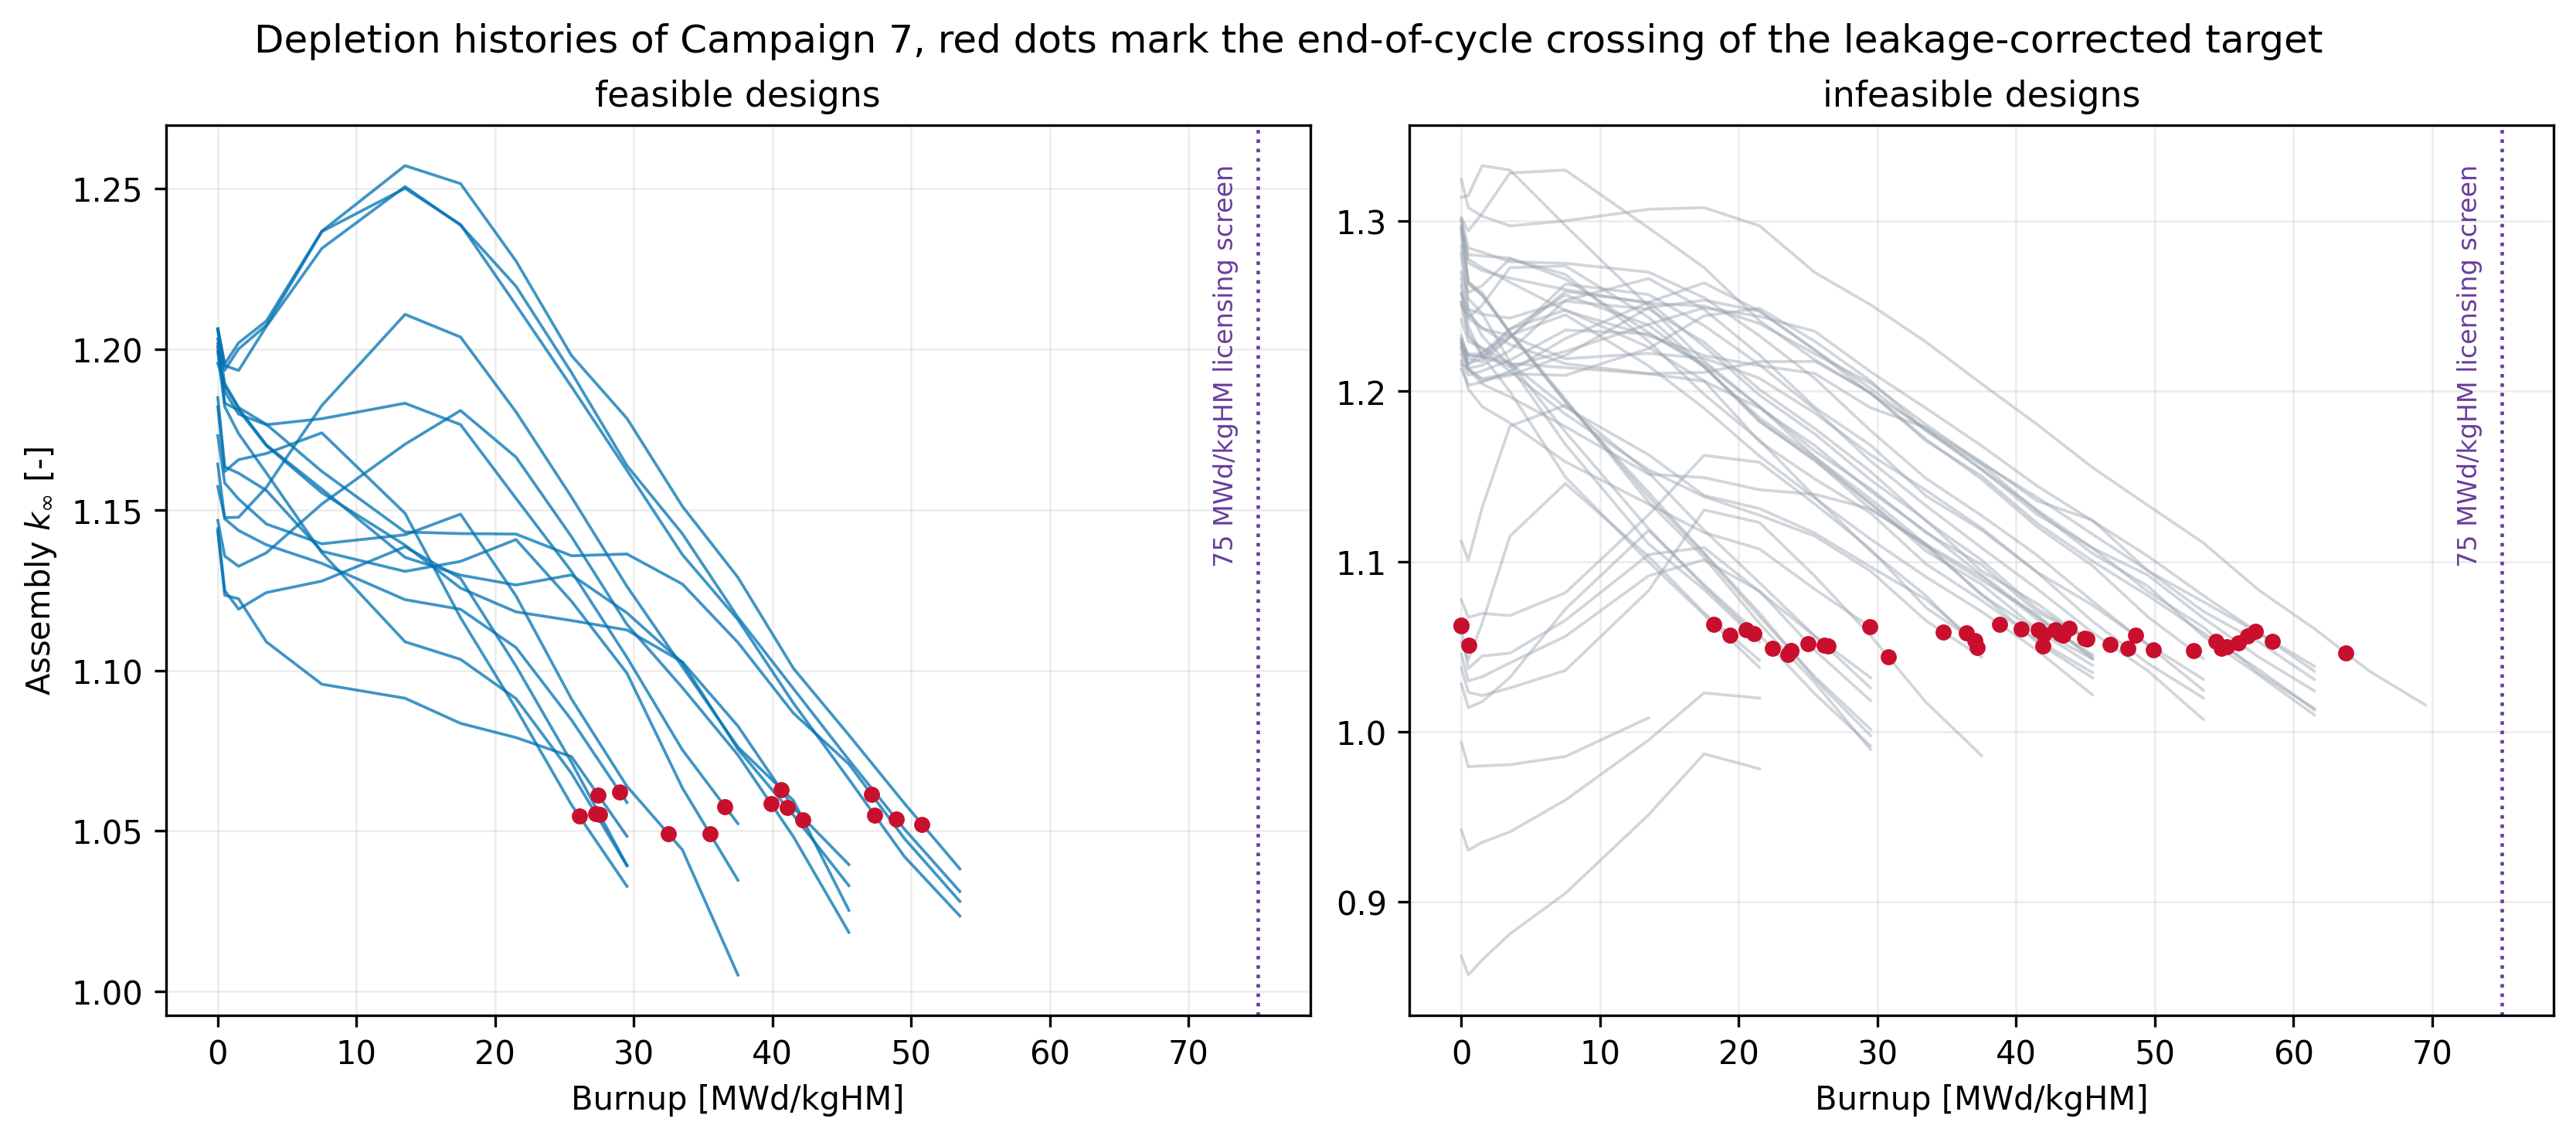
\includegraphics[width=\linewidth]{images/c7_kinf_histories}
  \caption{Assembly infinite multiplication factor against burnup for
  every Campaign 7 design, feasible designs on the left. Red markers
  are the end-of-cycle crossings of the leakage-corrected target. The
  gadolinium burnout maximum is visible between 13 and
  \SI{17}{MWd/kgHM}, and no design approaches the \SI{75}{MWd/kgHM}
  screen.}
  \label{fig:c7-histories}
\end{figure}

The reconstruction was validated against the archive. Taking the last
descending crossing of the target reproduces the stored end-of-cycle
burnup of all 57 crossing designs to within \SI{0.0011}{MWd/kgHM}. The
last crossing is the correct rule because the gadolinium burnout makes
the early history non-monotonic. The three designs without a crossing
are the two subcritical cores at zero cycle length and one design
ending at 55 EFPD.

Three facts follow from the figure. The gadolinium hump raises
$k_\infty$ by up to 0.06 before the decline. The highest end-of-cycle
burnup in the campaign is \SI{63.8}{MWd/kgHM}, so the
\SI{75}{MWd/kgHM} discharge screen of Section~\ref{sec:meth-atf} is
inactive and no design is censored, unlike Campaign 6. And the local
slope at end of cycle is steep, which governs the statistical error on
the cycle length.

The Monte Carlo error on the cycle length is obtained by propagating
the uncertainties of the two transport states that bracket the
crossing.

\begin{equation}
\sigma_B^2 = \left(\frac{\Delta B\,(k_\mathrm{t} - k_{j+1})}{(k_j - k_{j+1})^2}\right)^2 \sigma_{k_j}^2
+ \left(\frac{\Delta B\,(k_j - k_\mathrm{t})}{(k_j - k_{j+1})^2}\right)^2 \sigma_{k_{j+1}}^2
\label{eq:sigma-beoc}
\end{equation}

\noindent where the symbols have the following meaning.

\begin{itemize}
  \item $\sigma_B$ is the statistical uncertainty of the end-of-cycle
        burnup, in MWd/kgHM.

  \item $\Delta B$ is the burnup step between the two bracketing
        states, in MWd/kgHM.

  \item $k_j$ and $k_{j+1}$ are the infinite multiplication factors at
        the states before and after the crossing, dimensionless.

  \item $k_\mathrm{t}$ is the leakage-corrected target, dimensionless,
        treated as exact.

  \item $\sigma_{k_j}$ and $\sigma_{k_{j+1}}$ are the reported Monte
        Carlo standard deviations of the two states, dimensionless.
\end{itemize}

The cycle length follows from the specific power.

\begin{equation}
\sigma_\mathrm{EFPD} = \frac{1000\,\sigma_B}{P_\mathrm{sp}}
\label{eq:sigma-efpd}
\end{equation}

\noindent where the symbols have the following meaning.

\begin{itemize}
  \item $\sigma_\mathrm{EFPD}$ is the statistical uncertainty of the
        cycle length, in effective full power days.

  \item $P_\mathrm{sp}$ is the specific power of the core,
        \SI{9.98}{W/gHM}.
\end{itemize}

\begin{figure}[htbp]
  \centering
  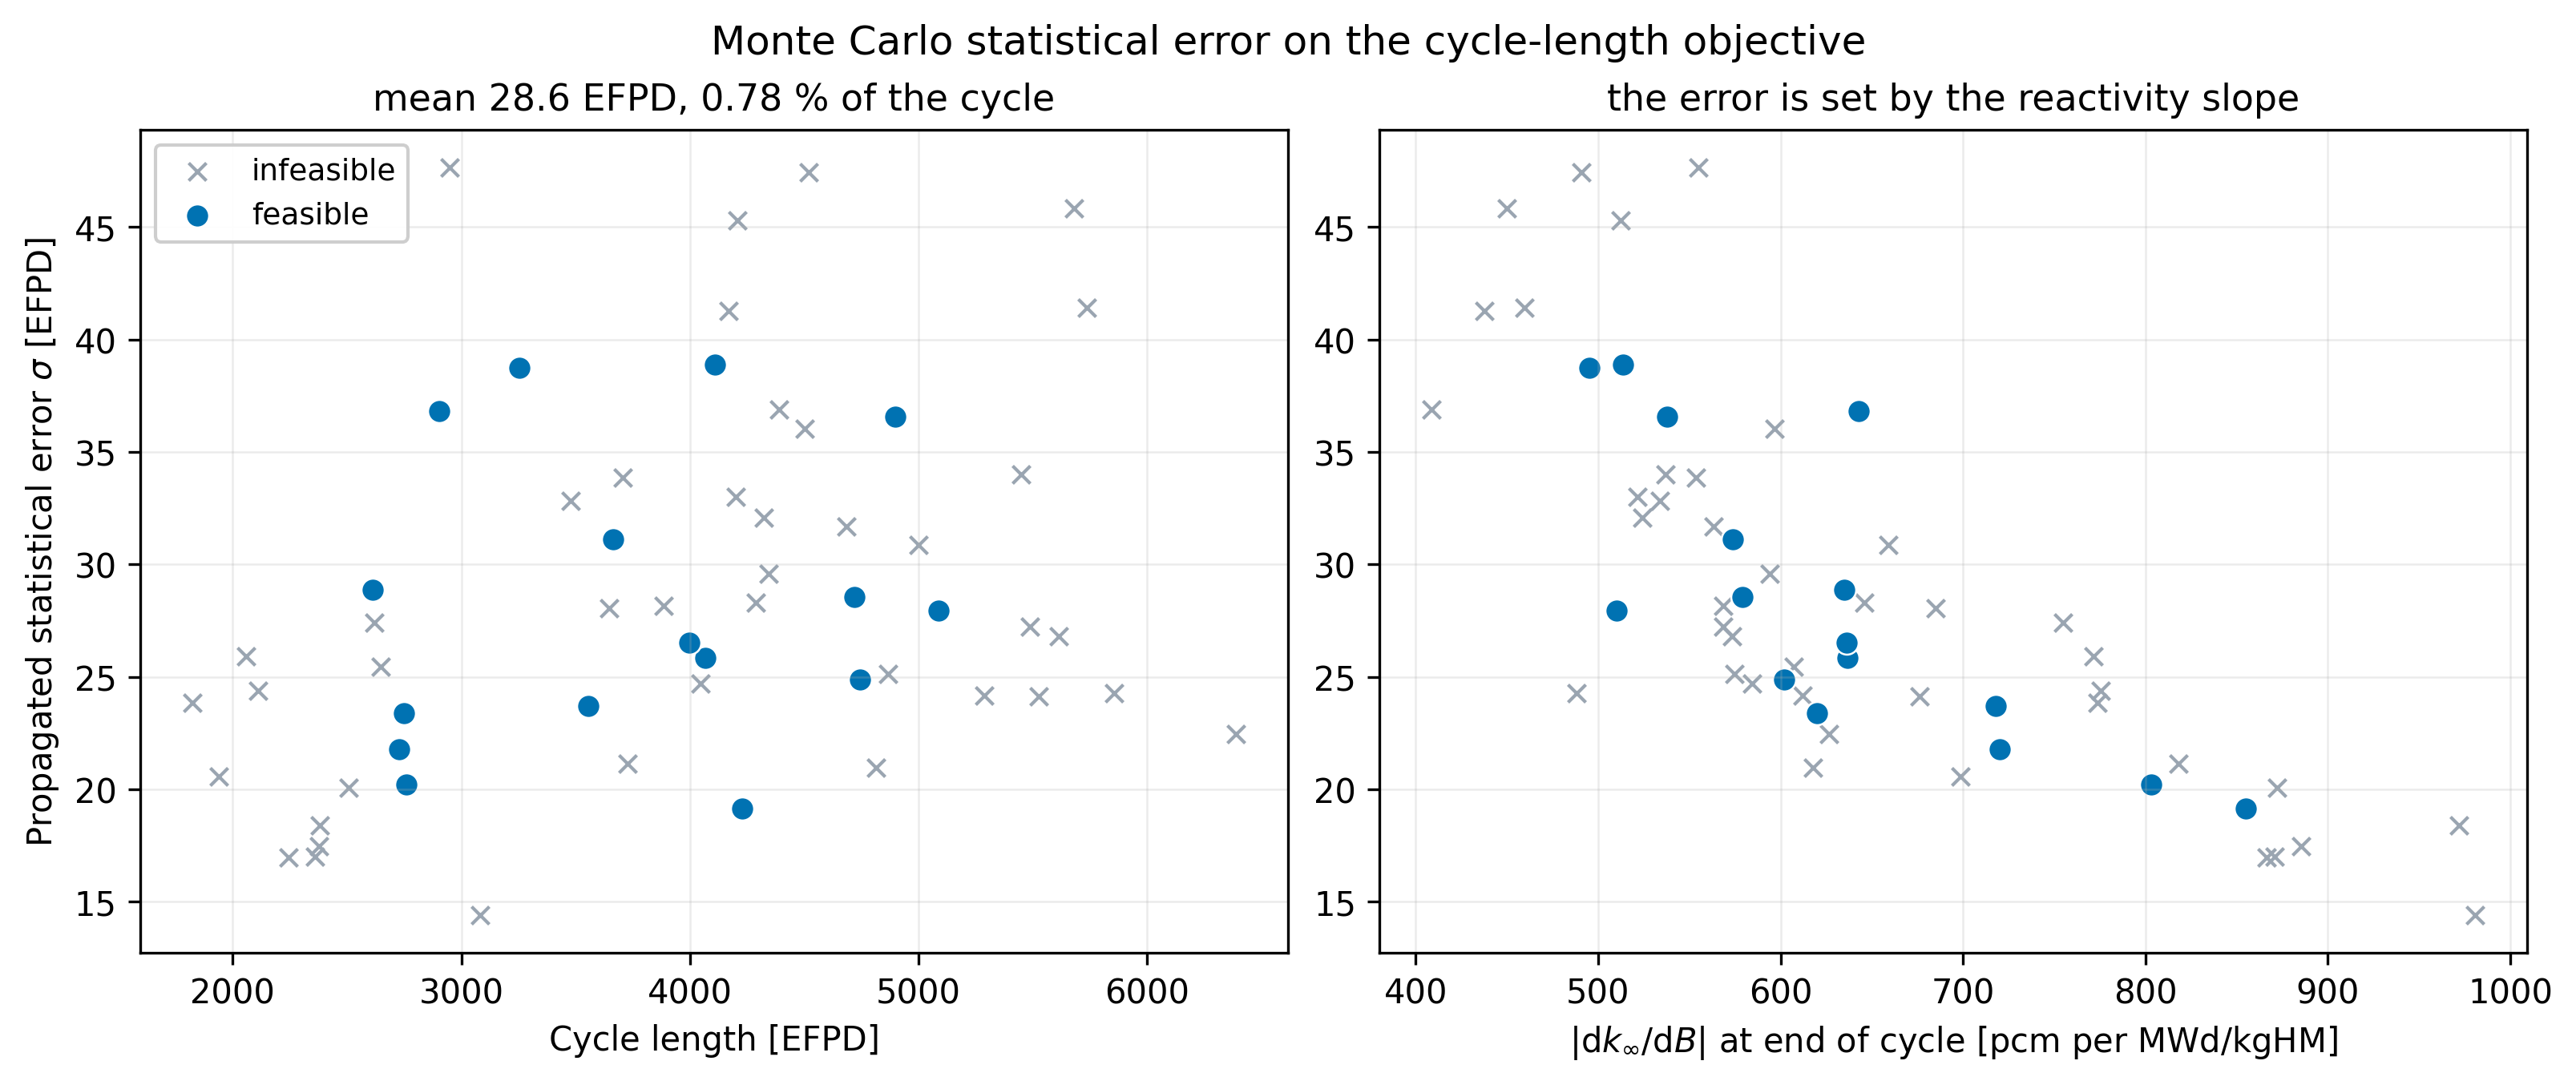
\includegraphics[width=\linewidth]{images/c7_cycle_uncertainty}
  \caption{Propagated Monte Carlo error on the cycle length against the
  cycle length and against the reactivity slope at end of cycle. The
  error is set by the slope, not by the length of the cycle.}
  \label{fig:c7-uncertainty}
\end{figure}

Table~\ref{tab:c7-uncertainty} summarises the result and
Figure~\ref{fig:c7-uncertainty} shows it. The slope at end of cycle
lies between 409 and \SI{981}{pcm} per MWd/kgHM with a median of 607.
The resulting error has a mean of 28.6 EFPD, \SI{0.78}{\%} of the
cycle, and a worst case of 47.7 EFPD, \SI{1.62}{\%}. On the six front
designs it is 25 to 37 EFPD. The smallest gap between adjacent front
designs is 154 EFPD, about five standard deviations, so the ordering of
the front in cycle length is statistically resolved.

\begin{table}[htbp]
  \centering
  \caption{Statistical error on the cycle length over the 57 designs
  with a resolved end-of-cycle crossing.}
  \label{tab:c7-uncertainty}
  \begin{tabular}{lccc}
    \toprule
    Quantity & Minimum & Median & Maximum \\
    \midrule
    Slope at end of cycle [pcm per MWd/kgHM] & 409 & 607 & 981 \\
    Bracketing sigma on $k_\infty$ [pcm]     & 178 & 218 & 274 \\
    $\sigma_\mathrm{EFPD}$ [d]               & 14.4 & 27.2 & 47.7 \\
    $\sigma_\mathrm{EFPD}$ as a fraction of the cycle [\%] & 0.35 & 0.74 & 1.62 \\
    \bottomrule
  \end{tabular}
\end{table}

The peaking axis is the opposite case. The front designs are separated
by 0.003 to 0.036 in $F_{\Delta H}$, the entropy study of
Section~\ref{sec:res-c6} bounded the systematic shift at $\pm 0.02$,
and no statistical error on the core peaking tally has been measured.
The ordering of the front in peaking is therefore not resolved, and
designs 59, 57 and 55 at 1.525, 1.528 and 1.529 must be treated as
indistinguishable until the tally errors are read from the statepoints.

\openpoint{Measure $\sigma(F_{\Delta H})$ from the per-bin relative
errors of the core mesh tally on the six front designs, or by seed
replicates, before any ordering claim on the peaking axis is made.}

\subsection{Cost and instrumentation}
\label{sec:res-c7-cost}

The campaign cost \SI{56965}{s} of wall time, \SI{949}{s} per
evaluation, against \SI{840}{s} in Campaign 6. The difference is the
control solve. Two instrumentation defects were found while reading
the archive, and both are recorded because they affect numbers reported
elsewhere in this chapter.

\begin{enumerate}
  \item The per-evaluation cost stored in the archive excludes the
        control solve, because that solve is invoked after the three
        timers close. Over the campaign the control solves are
        \SI{11}{\%} of the true cost and \SI{12.6}{\%} of the reported
        cost. The wall-clock figure of the block log is correct and is
        the one quoted above. The evaluator is corrected from Campaign
        8 (Section~\ref{sec:meth-cost}).

  \item The per-case parser of the run log never matched a single case
        line of any campaign, because the censoring marker inserted
        after the cycle length was not anticipated by its regular
        expression. The failure was silent, and every per-case table
        the parser produced before the correction was empty. No number
        in this chapter depends on that table, since all per-design
        quantities are read from the archive.
\end{enumerate}

\subsection{Limitations and what carries forward}
\label{sec:res-c7-limits}

Four limitations bound the claims of this section.

\begin{enumerate}
  \item Four designs, 10, 32, 41 and 43, reached the active batches
        with the Shannon entropy of the fission source not yet
        converged, the worst at 105 of 60 inactive batches. None is on
        either front. Their eigenvalues and peaking values carry an
        unquantified bias, are retained in the archive statistics of
        this section with that caveat, and are excluded from any
        candidate list.

  \item Twenty-five of the 60 designs have a pitch below
        \SI{1.2242}{cm}, twice the guide-tube outer radius. Below that
        value the lattice clips the guide-tube wall at the cell
        boundary silently, replacing up to \SI{27}{\%} of the wall
        cross-section by moderator at the box minimum of
        \SI{1.150}{cm}. Designs 57 and 59, the two lowest-peaking
        designs of the control-screen front, are both in the affected
        band. The same defect reaches back to every earlier campaign
        design at pitches below \SI{1.2242}{cm}, including the
        Campaign 4 infill designs pinned at the box minimum and the
        Campaign 6 discharge-screen champion at \SI{1.150}{cm}. Fixing
        the pitch at \SI{1.26}{cm} in Campaign 8 removes the defect
        prospectively, and a caveat is added to the affected results.

  \item The statistical error on the peaking objective is not
        measured, as stated above.

  \item Every cycle length in this campaign, as in all earlier ones, is
        a two-dimensional value. The axial leakage study of
        Section~\ref{sec:meth-lax}, completed after this campaign,
        measured the axial correction at \num{1.0282} to \num{1.0298}
        on six Campaign 6 designs, about \SI{3000}{pcm} of reactivity,
        which at the end-of-cycle slopes measured here corresponds to
        roughly 450 to 500 EFPD. Campaign 7 cycle lengths are therefore
        overstated by that amount relative to a finite-height core,
        uniformly across the archive, and the ordering of the front is
        unaffected. Campaign 8 carries the correction inside the
        end-of-cycle target from the start.
\end{enumerate}

What carries forward is the constraint architecture. The measured
control screen replaces the derived ceiling as the reactivity
constraint that does the work, a second reading with only the first two
banks inserted is added and recorded, the axial factor enters the
target, the acquisition settings of Campaign 6 are restored explicitly,
and the pitch is fixed at the value that both closes the geometric
defect and matches the reference fuel design. Section~\ref{sec:res-c8}
states the campaign built on those decisions.
 at that point.
%
%  Figures: copy the eight PDF files of c7_analysis_60/ into images/.
%    c7_pareto_60, c7_ctrl_screen, c7_rod_worth, c7_rodded_peaking,
%    c7_kinf_histories, c7_cycle_uncertainty, c7_infill_diversity,
%    c7_vars_influence
%
%  Labels defined here: sec:res-c7, sec:res-c7-basis, sec:res-c7-blocks,
%  sec:res-c7-screens, sec:res-c7-worth, sec:res-c7-rodded,
%  sec:res-c7-uncertainty, sec:res-c7-cost, sec:res-c7-limits,
%  tab:c7-blocks, tab:c7-front, tab:c7-nesting, tab:c7-uncertainty,
%  fig:c7-diversity, fig:c7-screens, fig:c7-pareto, fig:c7-worth,
%  fig:c7-influence, fig:c7-rodded, fig:c7-histories, fig:c7-uncertainty,
%  eq:g-ctrl, eq:k-implied, eq:bank-worth, eq:sigma-beoc, eq:sigma-efpd
%
%  Labels used from elsewhere: sec:meth-ctrl, sec:meth-ktarget,
%  sec:meth-acq, sec:res-c6, sec:res-c6-blocks, tab:fidelity,
%  sec:meth-lax, sec:res-c8, sec:meth-cost. Define sec:meth-ctrl,
%  sec:meth-lax and sec:meth-cost with methodology_c78_additions.tex.
%
%  Style: short paragraphs, no semicolons, no em dashes, every displayed
%  formula followed by a term list with units, enumerations as lists.
% =====================================================================

\section{Campaign 7: the controllability screen}
\label{sec:res-c7}

Campaign 6 closed with a front whose long-cycle end rode the
reactivity ceiling, and with the observation that the ceiling of 1.35
proxied controllable excess reactivity without a rod model. Campaign 7
replaces the proxy by a measurement. Every evaluation now solves the
beginning-of-life core a second time with the sixteen regulating-bank
control rod assemblies inserted, and the resulting eigenvalue enters the
constraint set directly. The campaign ran 60 evaluations on the AWS
instance in \SI{15.82}{h}, and every one of them completed without
error.

\subsection{The one change and its two consequences}
\label{sec:res-c7-basis}

The constraint added is the controllability screen of
Section~\ref{sec:meth-ctrl}.

\begin{equation}
g_\mathrm{ctrl}(\mathbf{x}) = k_\mathrm{ARI}(\mathbf{x}) - (1 - \Delta\rho_\mathrm{op}) \le 0
\label{eq:g-ctrl}
\end{equation}

\noindent where the symbols have the following meaning.

\begin{itemize}
  \item $k_\mathrm{ARI}$ is the effective multiplication factor of the
        32-assembly core at beginning of life with all sixteen
        regulating-bank assemblies inserted and the shutdown banks
        withdrawn, dimensionless.

  \item $\Delta\rho_\mathrm{op}$ is the operating subcriticality margin
        demanded of the regulating banks, \num{0.01} in units of $k$,
        that is \SI{1000}{pcm}.

  \item $\mathbf{x}$ is the design vector.
\end{itemize}

Two settings changed with it. The reactivity ceiling was lowered from
1.35 to 1.126, a value derived before the campaign from the smallest
regulating-bank worth measured on eight Campaign 6 designs, and the
enrichment cap was lowered to \SI{12}{wt\%} on the as-built peripheral
ring, giving a search box of 3.0 to \SI{10.43}{wt\%}. Both were
intended as consequences of the controllability requirement rather than
as independent changes, and the campaign tests whether they were
consistent with the measurement they were meant to anticipate.

\subsection{Design of experiments and the three infill blocks}
\label{sec:res-c7-blocks}

The campaign ran a design of experiments of 42 followed by three infill
blocks of six. Table~\ref{tab:c7-blocks} records the outcome of each
block and Figure~\ref{fig:c7-diversity} its diversity, measured as the
spread of each design variable within the block as a fraction of the
range spanned by the whole archive.

\begin{table}[htbp]
  \centering
  \caption{Campaign 7 blocks. The hypervolume is the frozen-reference
  value written at each block boundary. Spread is the within-block
  range of each variable as a fraction of the archive range, listed
  for the four non-geometric variables.}
  \label{tab:c7-blocks}
  \begin{tabular}{lccll}
    \toprule
    Block & Designs & Feasible & Hypervolume & Spread in $e_\mathrm{in}$, $e_\mathrm{out}$, $w_\mathrm{Gd}$, $n_\mathrm{Gd}$ \\
    \midrule
    DOE      & 42 & 13 & 773.7 & 0.98 to 1.00 \\
    Infill 1 &  6 &  0 & 773.7 & 0.000 to 0.002 \\
    Infill 2 &  6 &  3 & 996.5 & 0.07 to 0.29 \\
    Infill 3 &  6 &  0 & 996.5 & 0.015 to 0.13 \\
    \bottomrule
  \end{tabular}
\end{table}

\begin{figure}[htbp]
  \centering
  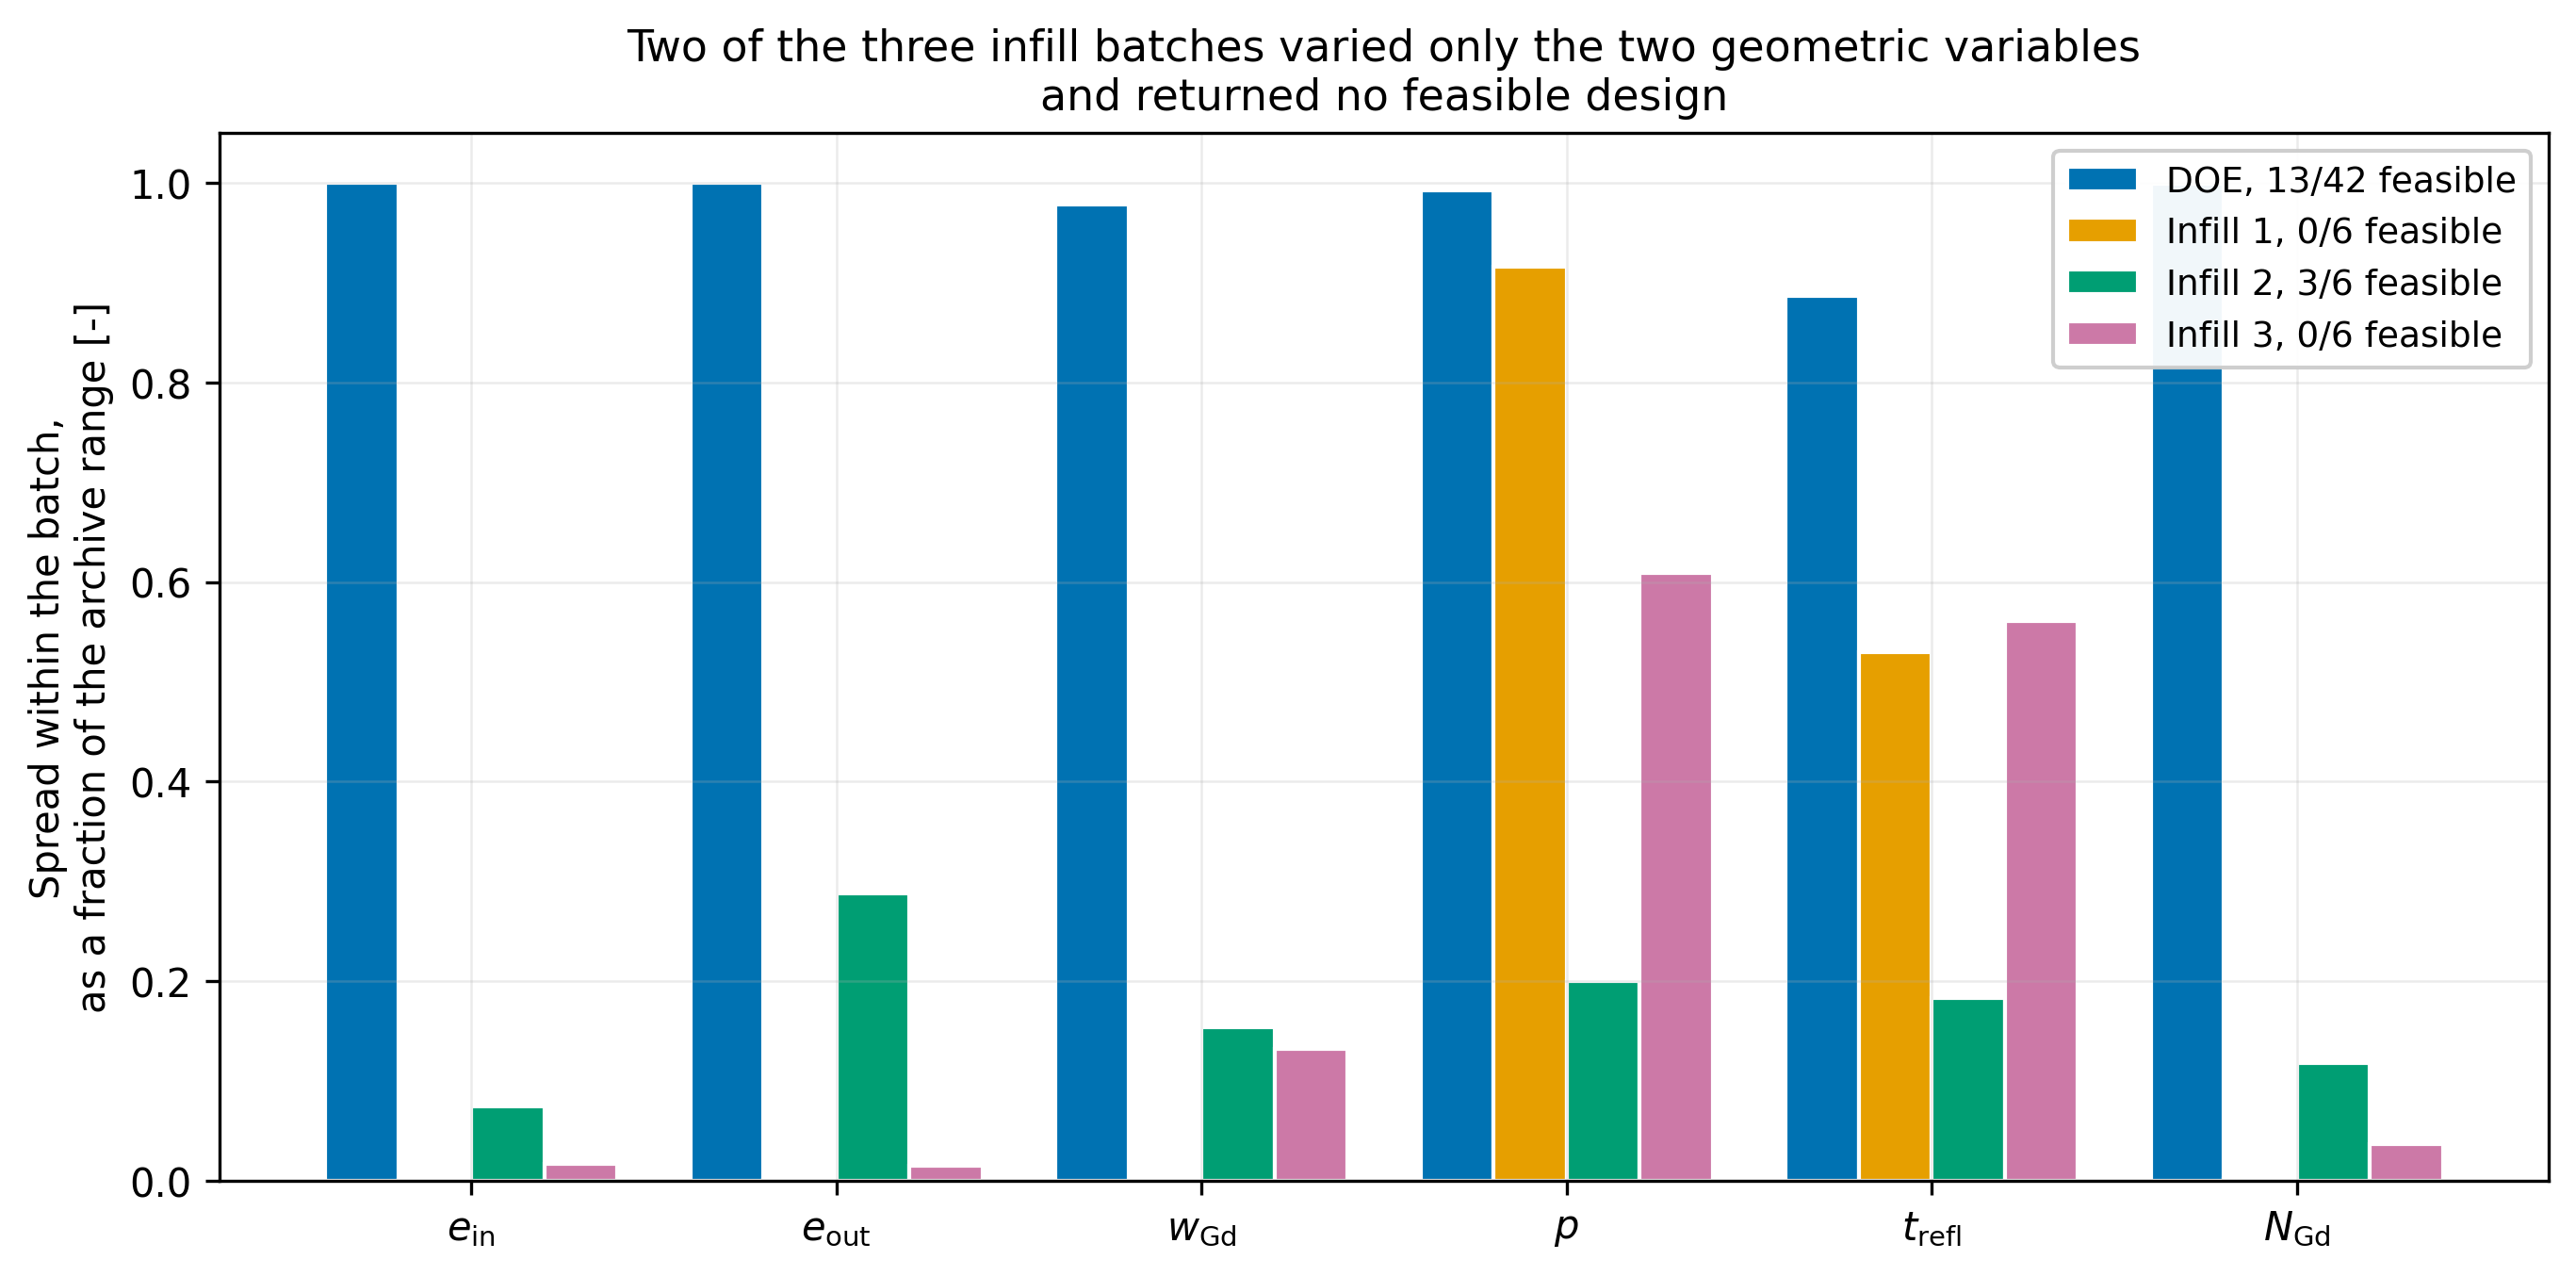
\includegraphics[width=\linewidth]{images/c7_infill_diversity}
  \caption{Within-block spread of each design variable, as a fraction
  of the archive range. Infill blocks 1 and 3 vary only the pitch and
  the reflector thickness, and neither returned a feasible design.}
  \label{fig:c7-diversity}
\end{figure}

Two of the three infill blocks collapsed. In block 1 the six designs
share one enrichment pair, \num{5.09} and \SI{4.04}{wt\%}, exactly zero
gadolinia and 24 poisoned pins, and differ only in pitch and reflector
thickness. In block 3 the same pattern recurs at \num{8.13} and
\SI{7.33}{wt\%} with 32 pins. All twelve designs of the two blocks
failed the reactivity ceiling.

The cause is a configuration regression, not a new defect. The
acquisition ran with a minimum separation of 0.05 and a feasibility
margin of 1.0 standard deviation, the default values of the launcher,
where Campaign 6 had established 0.14 and 1.5 in
Section~\ref{sec:res-c6-blocks}. The two collapsed blocks satisfied the
separation rule as coded, with pairwise separations of 0.059 to 0.089,
because the rule averages over all six variables and two of them
supplied the whole distance. A per-variable minimum spread would have
rejected both batches.

The consequence for the convergence record is that the flat
hypervolume of block 3 is not a stopping signal. Under the Campaign 6
rule a zero gain counts toward stopping only when the acquisition is
functioning, and block 3 demonstrably was not. The campaign therefore
ends with an unconverged front, and its value lies in the constraint
measurements rather than in the front itself.

\subsection{Feasibility and the nesting of the two screens}
\label{sec:res-c7-screens}

Of the 60 designs, 16 are feasible against all six constraints, a
fraction of \SI{26.7}{\%} against \SI{67}{\%} in the Campaign 6 design
of experiments. Table~\ref{tab:c7-nesting} gives the constraint census.
No design fails the enrichment or the geometric constraint, two fail
the peaking limit, nine fall below the reactivity floor, 34 exceed the
ceiling and 20 fail the controllability screen.

\begin{table}[htbp]
  \centering
  \caption{Constraint census of Campaign 7 and the joint activity of
  the two reactivity screens. Every design that fails the
  controllability screen also fails the derived ceiling, and fourteen
  designs fail the ceiling while passing the controllability screen.}
  \label{tab:c7-nesting}
  \begin{tabular}{lc}
    \toprule
    Outcome & Designs \\
    \midrule
    Fail $g_{k\max}$ at 1.126                      & 34 \\
    Fail $g_\mathrm{ctrl}$                         & 20 \\
    Fail $g_\mathrm{ctrl}$ and pass $g_{k\max}$    &  0 \\
    Fail $g_{k\max}$ and pass $g_\mathrm{ctrl}$    & 14 \\
    Pass every constraint except $g_{k\max}$       & 14 \\
    Feasible on all six                            & 16 \\
    \bottomrule
  \end{tabular}
\end{table}

\begin{figure}[htbp]
  \centering
  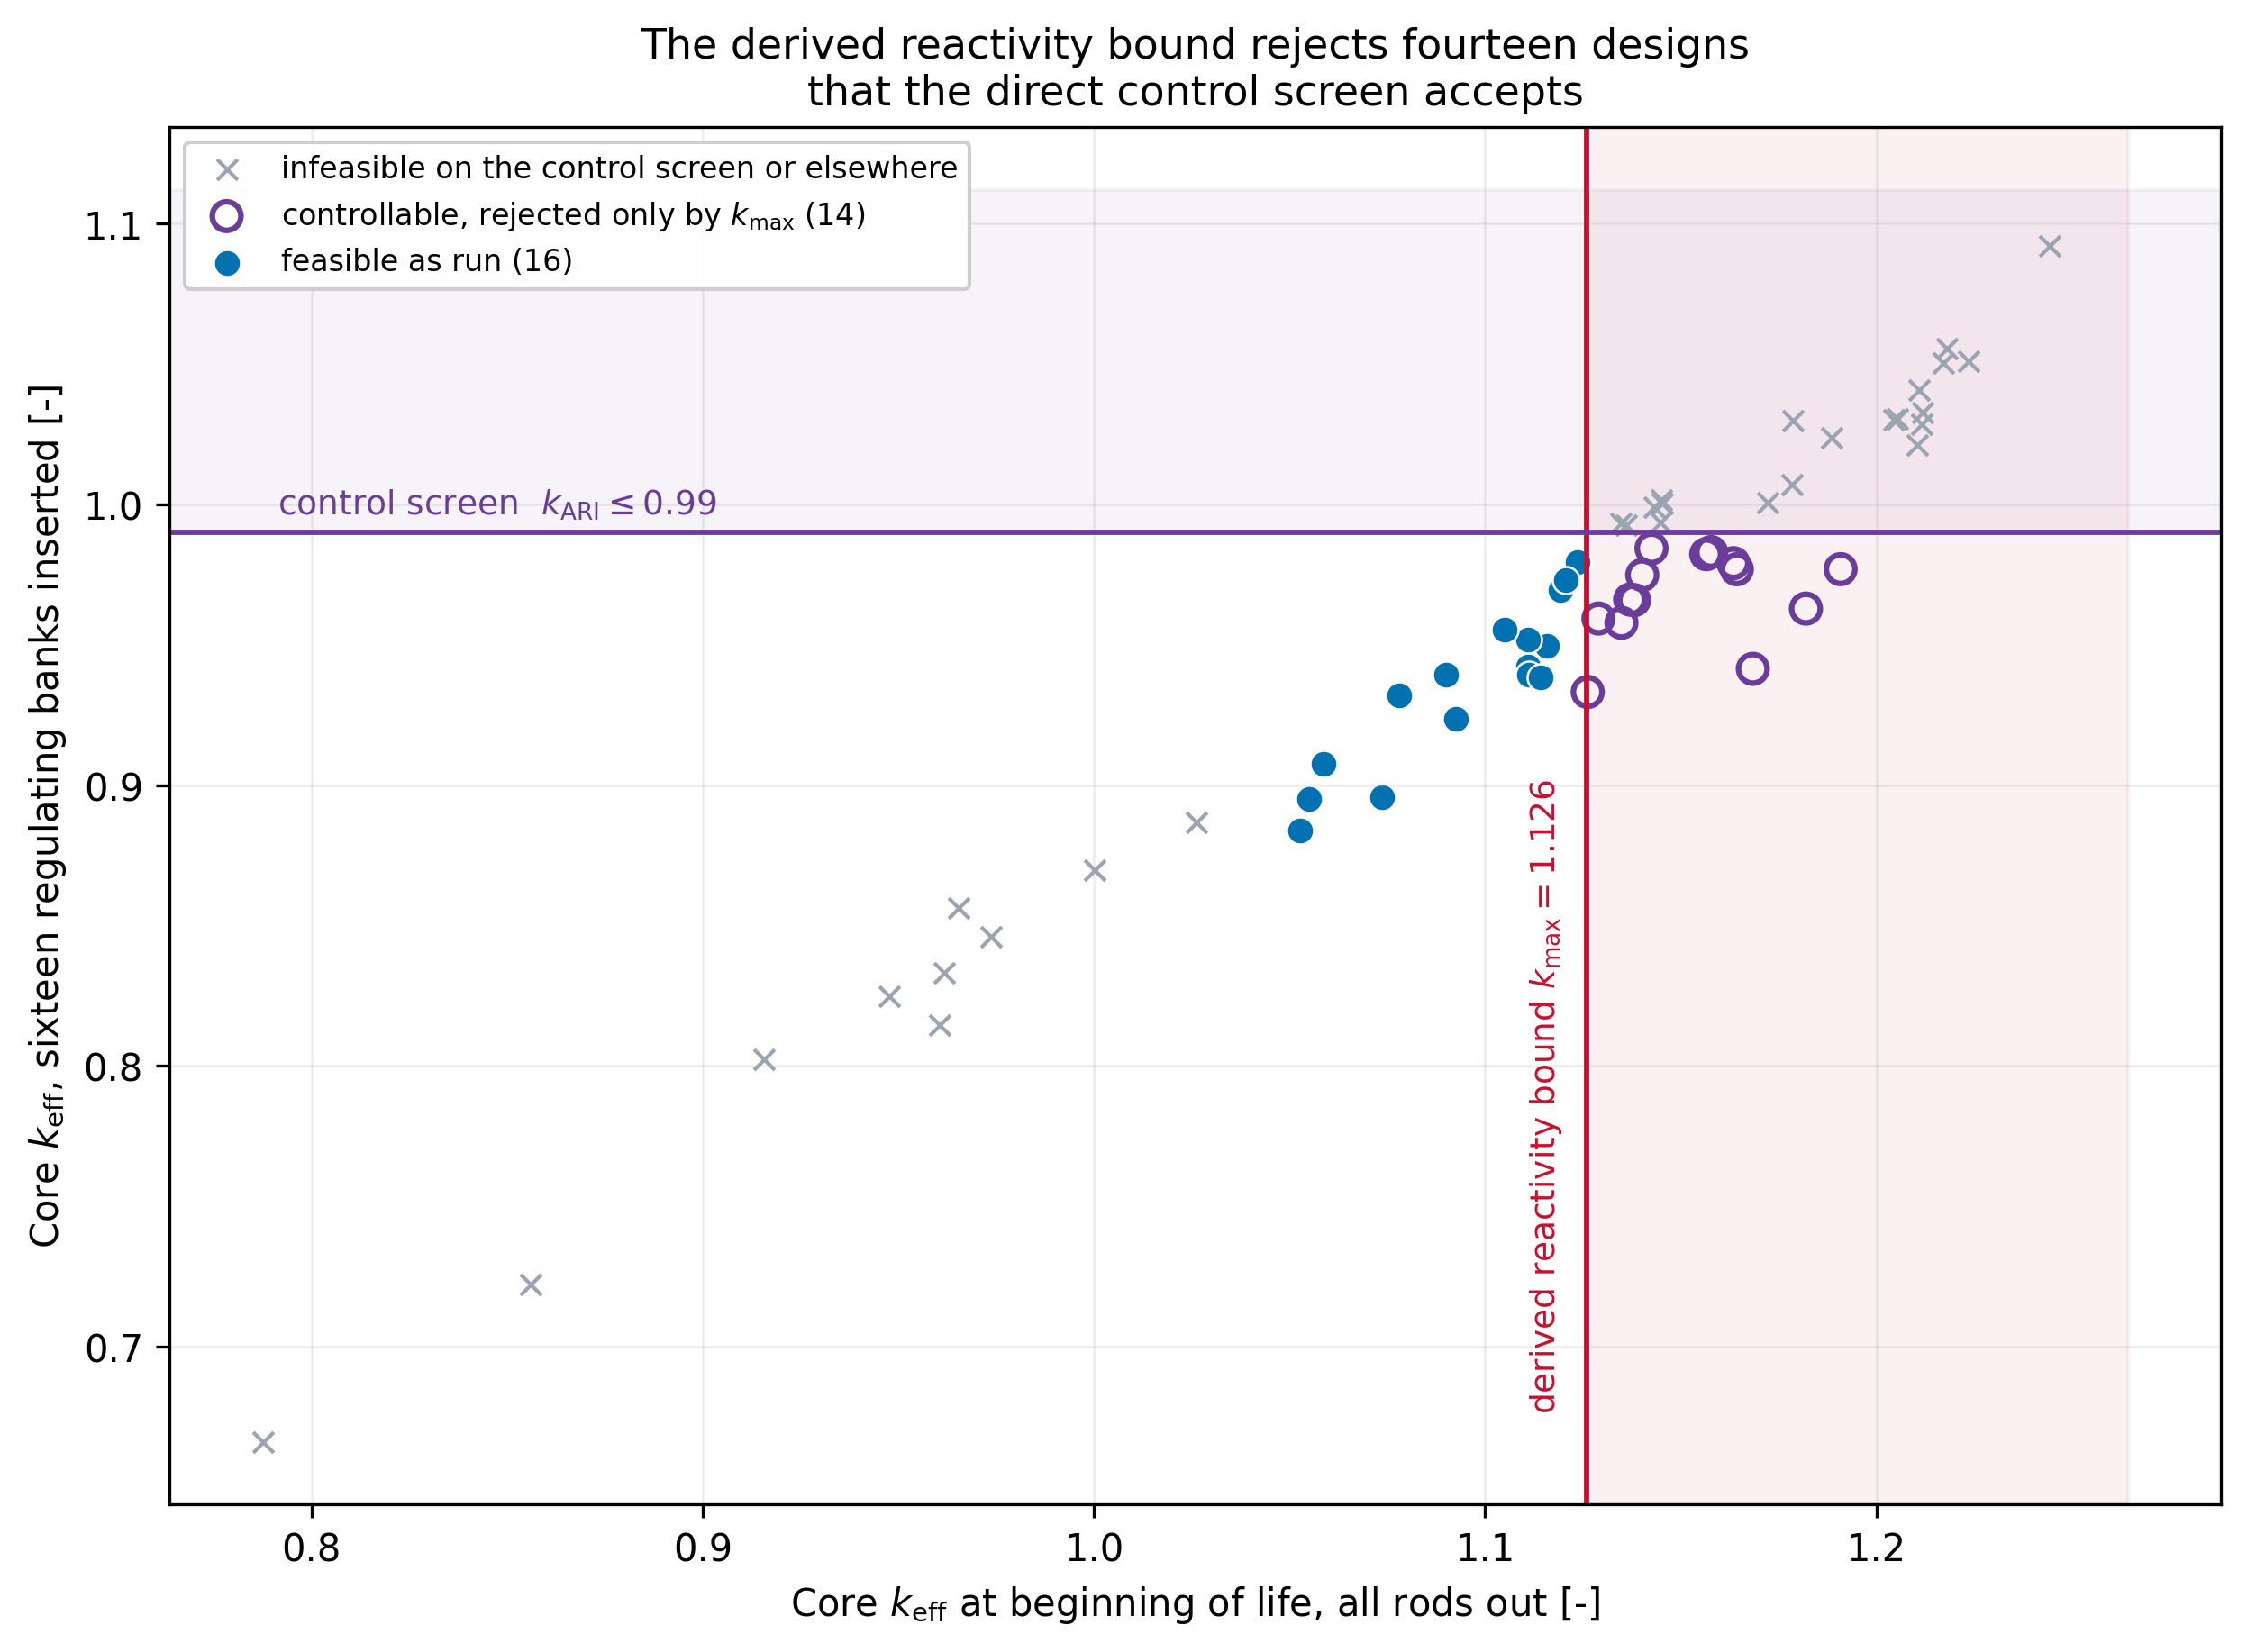
\includegraphics[width=0.9\linewidth]{images/c7_ctrl_screen}
  \caption{The two reactivity screens of Campaign 7 in the plane of
  the unrodded and the all-regulating-banks-in core eigenvalues. The
  derived ceiling at 1.126 rejects fourteen designs, marked by open
  circles, that the directly measured control screen accepts.}
  \label{fig:c7-screens}
\end{figure}

The two screens are nested. Not one design in the archive fails the
control screen without also failing the derived ceiling, and fourteen
designs fail the ceiling while their own measured bank worth shows them
controllable at the stated margin. Figure~\ref{fig:c7-screens} shows
the nesting directly. The ceiling of 1.126 therefore did no work that
the measurement did not do, and it discarded fourteen evaluations that
the measurement would have kept.

The derivation explains why. The eight Campaign 6 designs from which
1.126 was obtained had worths between \num{12174} and
\SI{12718}{pcm}, a spread of four per cent. The 60 designs of this
campaign span \num{10936} to \SI{22699}{pcm}, a factor of two. Eight
near-identical designs under-sampled the variability by an order of
magnitude, and the resulting bound is at once too tight where it
matters and not conservative in general. Restricted to the 22 designs
with an unrodded eigenvalue between 1.09 and 1.17, the smallest
measured worth of \SI{14126}{pcm} implies a ceiling of 1.151, while the
smallest worth in the whole archive implies 1.110.

The front reflects the same fact. As run, the feasible non-dominated set
holds three designs, all from infill block 2. With the derived ceiling
removed and the measured control screen retained, the feasible set grows
from 16 to 30 designs, the front doubles to six, the peaking floor moves
from 1.565 to 1.525, and the hypervolume against the frozen reference
rises from 996.5 to 1054.1, a gain of \SI{5.8}{\%}. Three of the six
designs come from infill block 3, the block that under the ceiling
contributed nothing. Table~\ref{tab:c7-front} lists both fronts and
Figure~\ref{fig:c7-pareto} places them in the objective plane.

\begin{table}[htbp]
  \centering
  \small
  \caption{The Campaign 7 front under the two screening rules. Designs
  48, 53 and 49 form the front as run. All six form the front when the
  measured control screen alone governs reactivity. Bank worth is the
  difference between the unrodded and the all-banks-in eigenvalues.}
  \label{tab:c7-front}
  \begin{tabular}{ccccccccccc}
    \toprule
    Design & EFPD & $F_{\Delta H}$ & $e_\mathrm{in}$ & $e_\mathrm{out}$ & $w_\mathrm{Gd}$ & $p$ & $t_\mathrm{refl}$ & $n_\mathrm{Gd}$ & $k_\mathrm{eff}^\mathrm{core}$ & worth \\
           & [d] & [-] & [wt\%] & [wt\%] & [wt\%] & [cm] & [cm] & [-] & [-] & [pcm] \\
    \midrule
    59 & 3886 & 1.525 & 8.13 & 7.33 & 1.10 & 1.150 & 19.49 & 32 & 1.135 & 17699 \\
    57 & 4045 & 1.528 & 8.13 & 7.33 & 1.21 & 1.176 & 17.87 & 32 & 1.137 & 17094 \\
    55 & 4502 & 1.529 & 8.14 & 7.34 & 1.10 & 1.238 & 14.09 & 32 & 1.143 & 15815 \\
    48 & 4745 & 1.565 & 8.71 & 7.80 & 1.93 & 1.237 & 14.06 & 40 & 1.119 & 14970 \\
    53 & 4899 & 1.590 & 8.97 & 7.88 & 1.96 & 1.249 & 13.21 & 40 & 1.121 & 14734 \\
    49 & 5087 & 1.598 & 9.19 & 8.30 & 2.13 & 1.267 & 12.29 & 40 & 1.124 & 14416 \\
    \bottomrule
  \end{tabular}
\end{table}

\begin{figure}[htbp]
  \centering
  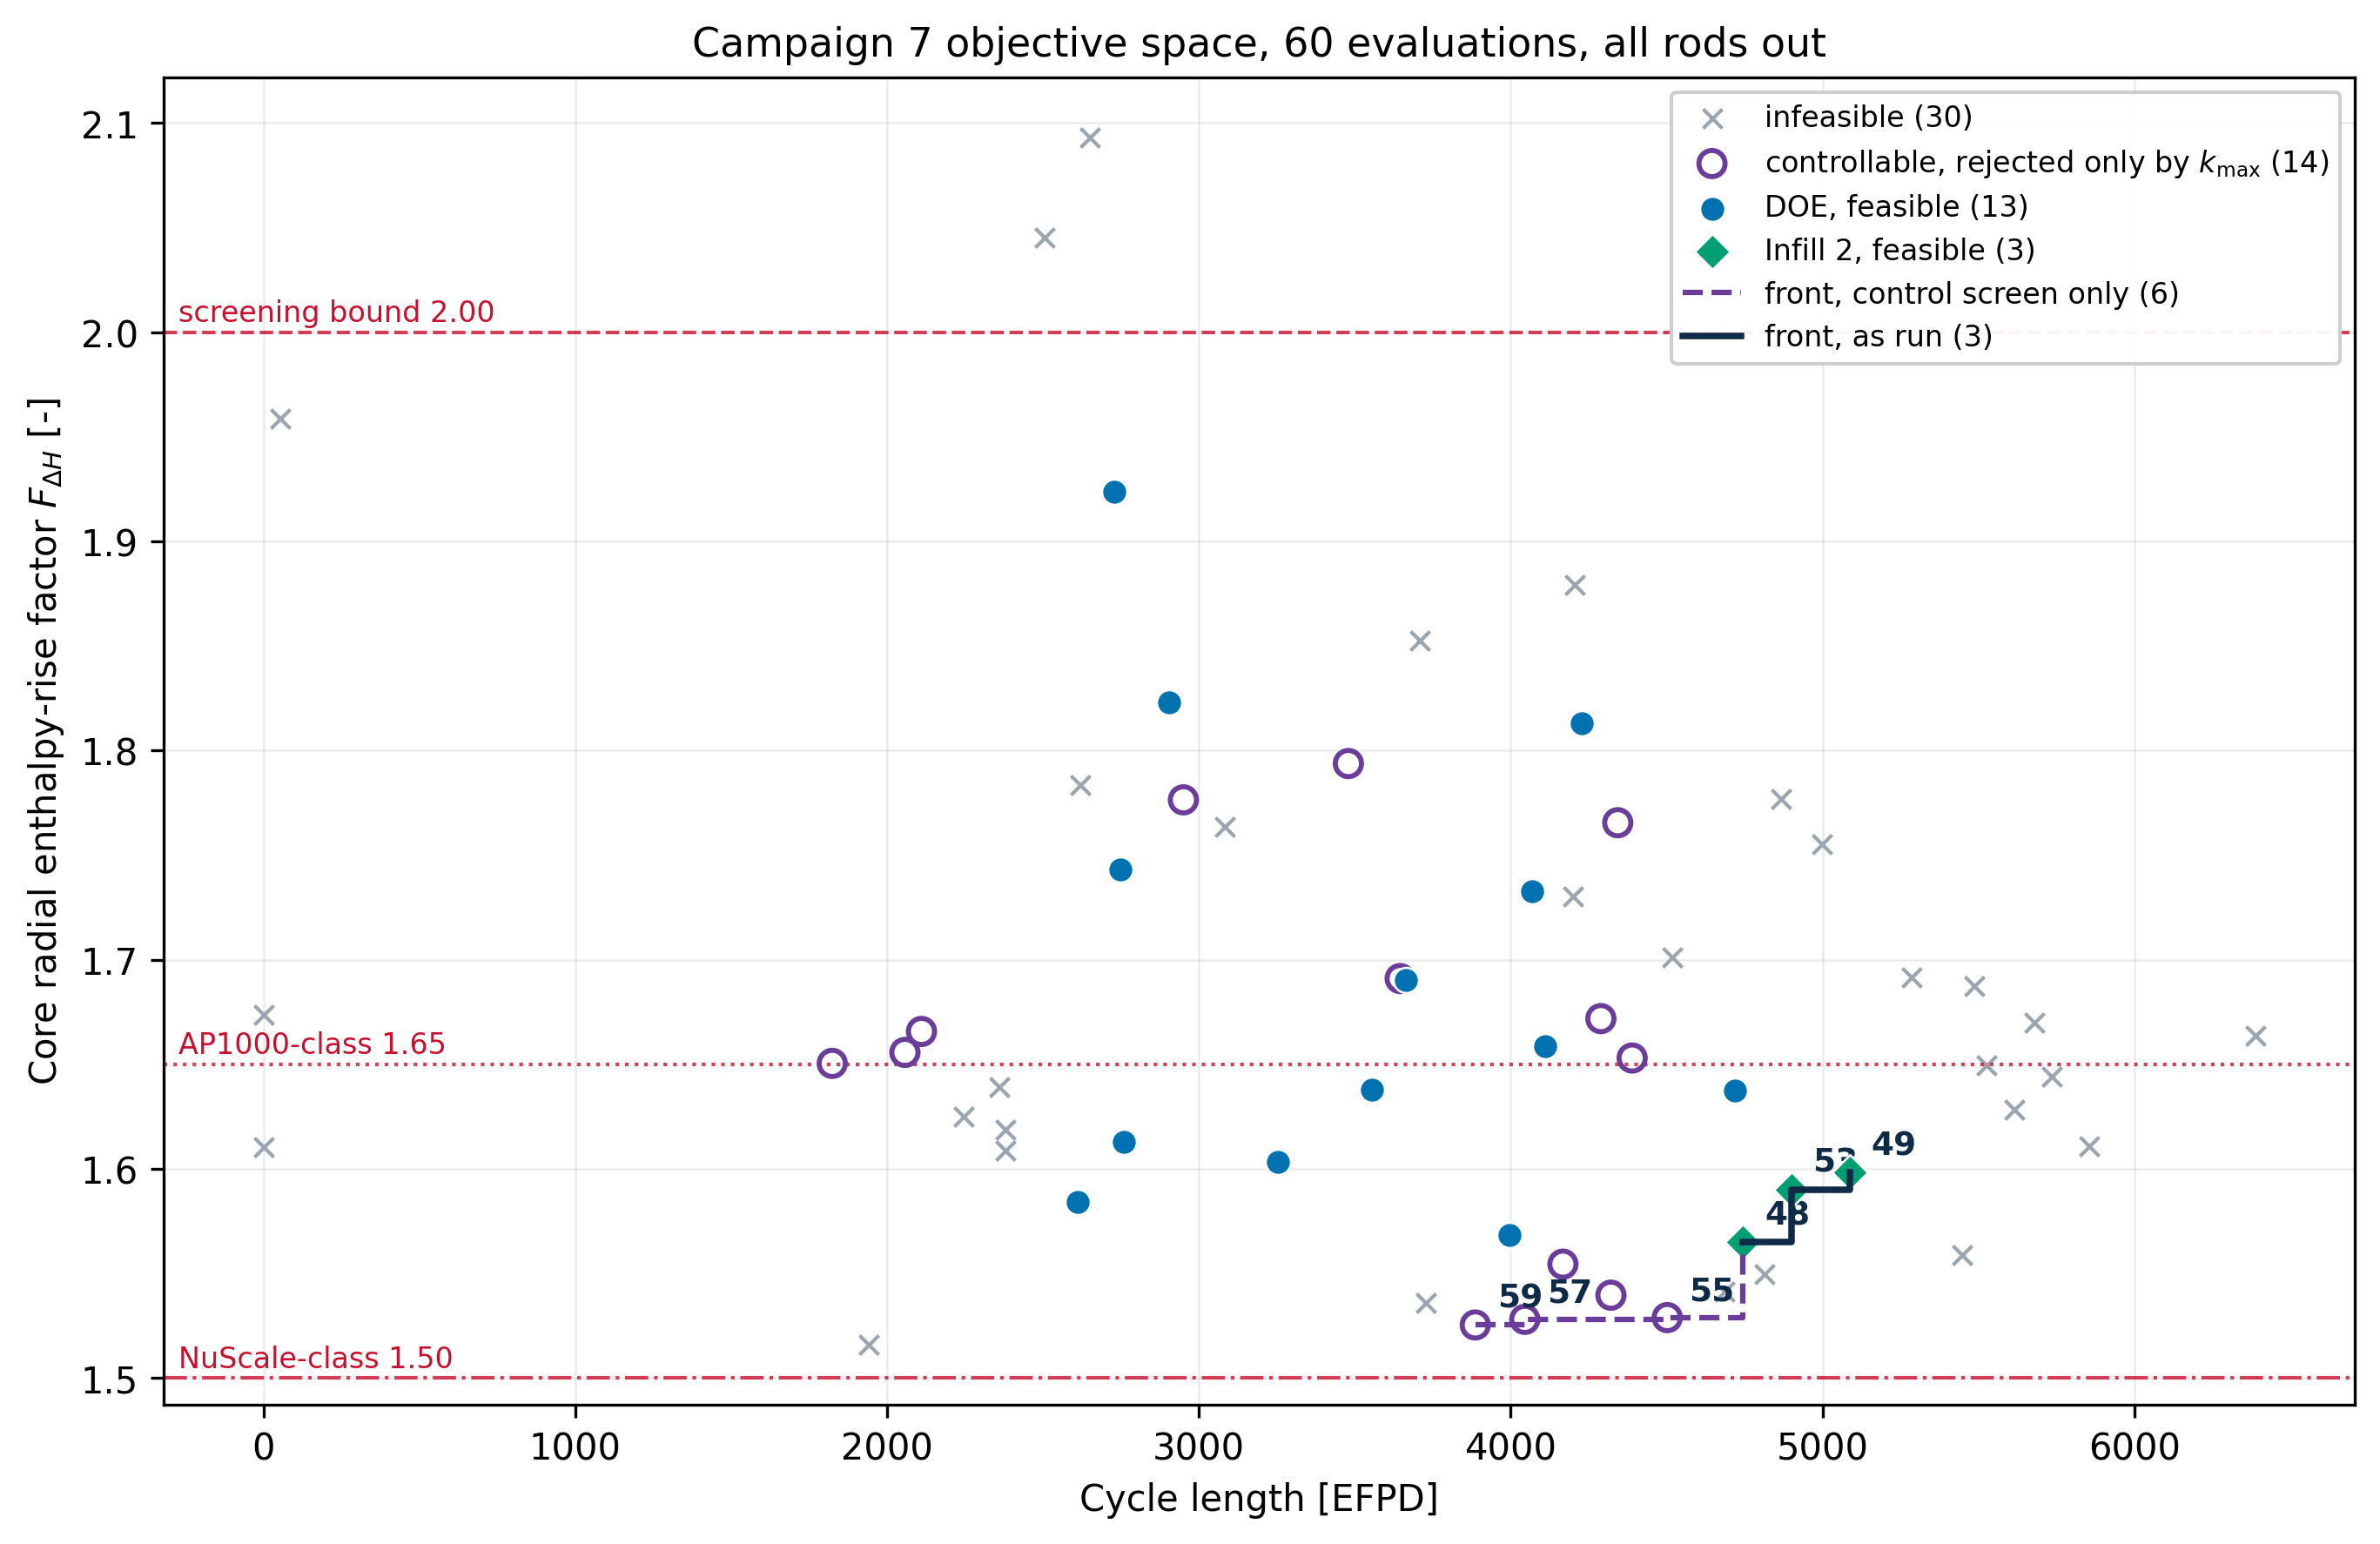
\includegraphics[width=\linewidth]{images/c7_pareto_60}
  \caption{Campaign 7 objective space with all rods out. Filled markers
  are feasible as run, open circles are controllable designs rejected
  only by the derived ceiling. The solid front is the one the campaign
  reported and the dashed front is the one the measured control screen
  supports.}
  \label{fig:c7-pareto}
\end{figure}

Two properties of the front as run deserve stating. Its three designs
sit \num{240} to \SI{680}{pcm} below the ceiling, so the front is a
constraint boundary and not an interior trade. And the cycle lengths
are not comparable with Campaign 6, because the enrichment box is a
different one, and the longest feasible cycle of 5087 EFPD says nothing
about the reactor class that the 9981 EFPD of Campaign 6 did not
already say.

%% AUTHOR: one paragraph on why the low-peaking end of the control-screen
%% front lives at thick reflectors and narrow pitch, and on the physical
%% meaning of a front that doubles when a surrogate bound is removed.

\subsection{Regulating-bank worth and the reason the screens nest}
\label{sec:res-c7-worth}

The worth of the sixteen regulating banks is defined on the two core
solves of every evaluation.

\begin{equation}
\rho_\mathrm{bank}(\mathbf{x}) = k_\mathrm{eff}^\mathrm{core}(\mathbf{x}) - k_\mathrm{ARI}(\mathbf{x})
\label{eq:bank-worth}
\end{equation}

\noindent where the symbols have the following meaning.

\begin{itemize}
  \item $\rho_\mathrm{bank}$ is the bank worth in units of $k$,
        dimensionless, reported in pcm by multiplying by $10^5$.

  \item $k_\mathrm{eff}^\mathrm{core}$ is the unrodded core eigenvalue
        at beginning of life, dimensionless.

  \item $k_\mathrm{ARI}$ is the eigenvalue with all sixteen regulating
        banks inserted, dimensionless.
\end{itemize}

Across the archive the worth ranges from \num{10936} to
\SI{22699}{pcm} with a median of \SI{16510}{pcm}. Figure~\ref{fig:c7-worth}
shows its two strongest drivers and Figure~\ref{fig:c7-influence} the
rank correlations of all six variables with the objectives, the worth
and the rodded peaking.

\begin{figure}[htbp]
  \centering
  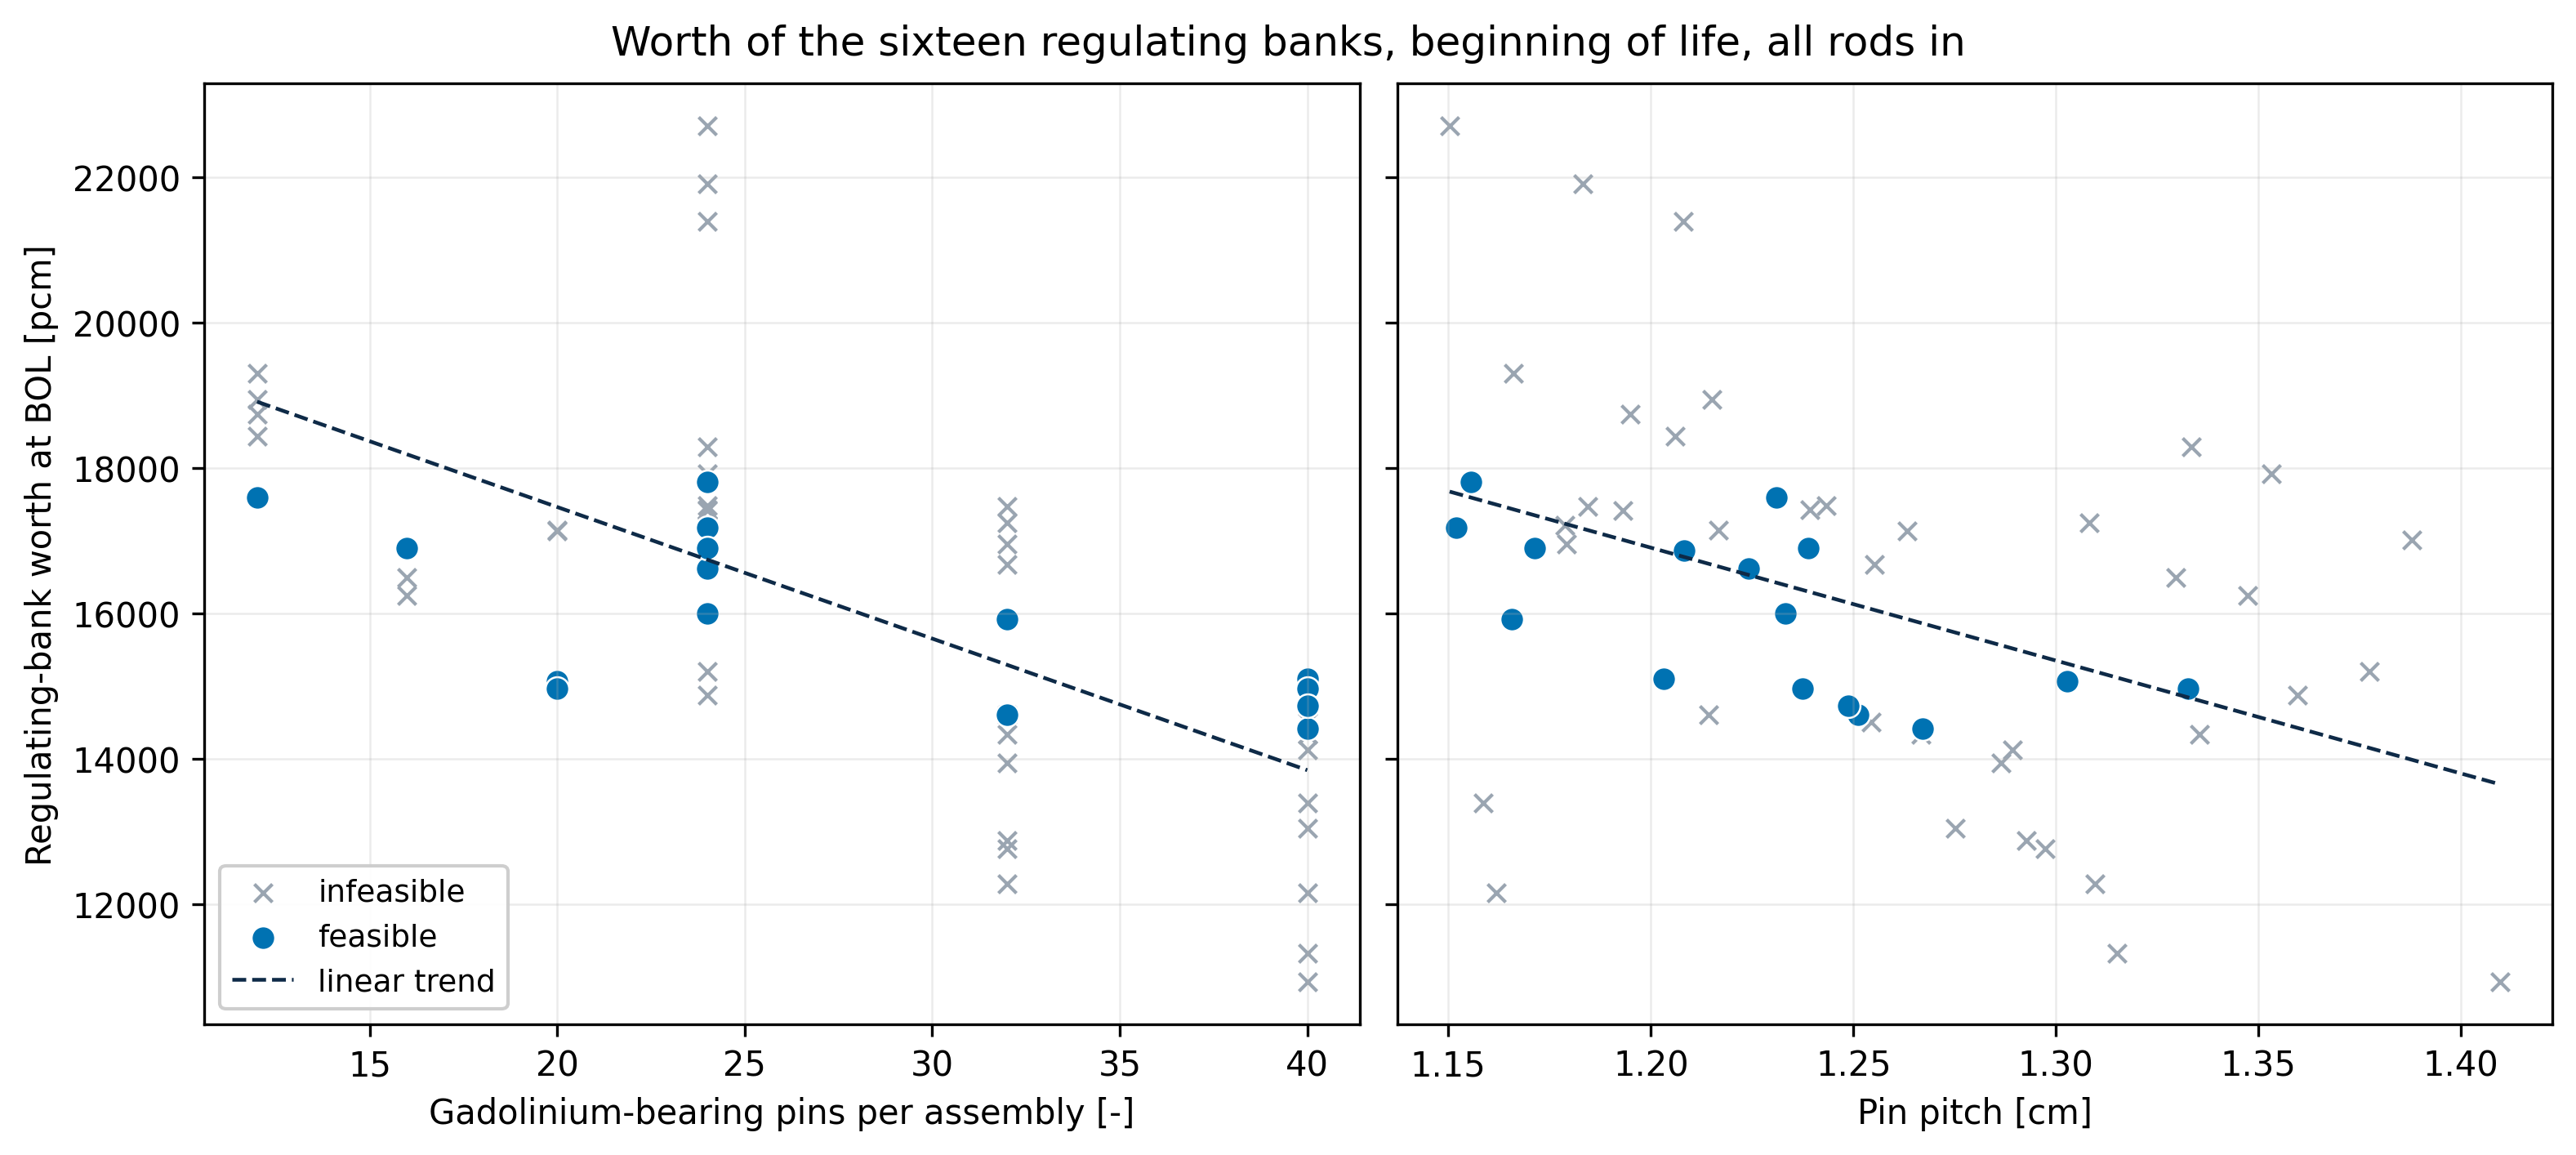
\includegraphics[width=\linewidth]{images/c7_rod_worth}
  \caption{Worth of the sixteen regulating banks against the
  gadolinium pin count and the pin pitch. The dashed lines are
  least-squares trends and serve only as visual guides.}
  \label{fig:c7-worth}
\end{figure}

\begin{figure}[htbp]
  \centering
  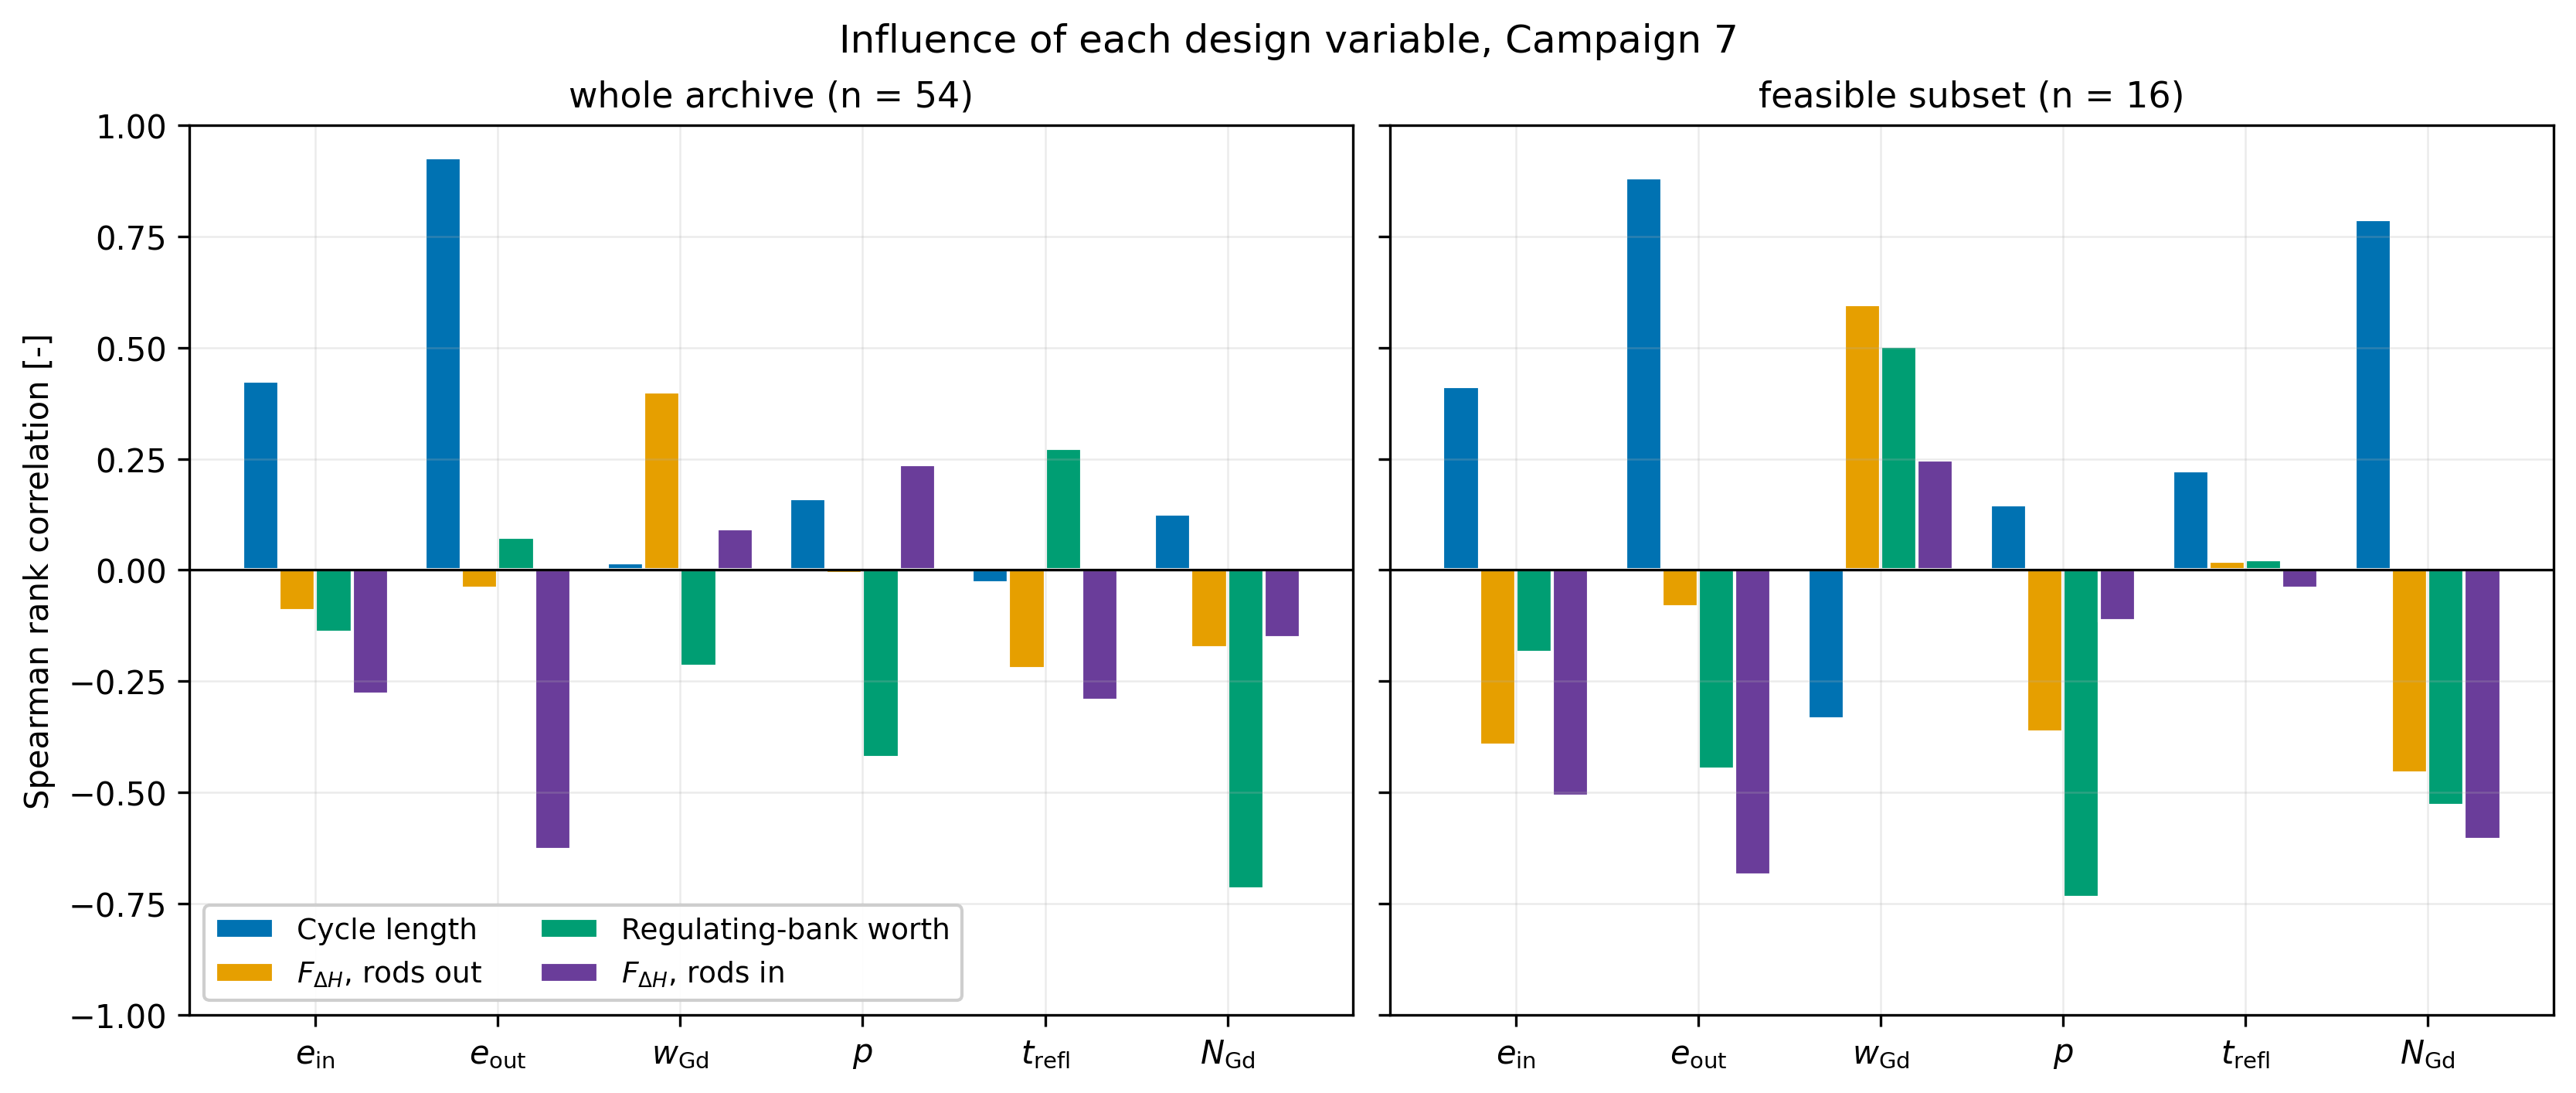
\includegraphics[width=\linewidth]{images/c7_vars_influence}
  \caption{Spearman rank correlation of each design variable with the
  two objectives, the regulating-bank worth and the peaking with the
  banks inserted, over the whole archive and over the feasible subset.}
  \label{fig:c7-influence}
\end{figure}

The worth correlates at $-0.68$ with the gadolinium pin count, at
$-0.45$ with the pitch and at $+0.61$ with the unrodded eigenvalue.
Gadolinium depresses the eigenvalue and the bank worth together, so the
designs with the least worth are the heavily poisoned ones, which are
already far below the ceiling for a different reason. That is why the
two screens nest in this design space, and it is also why the
eight-design derivation of the ceiling looked safe when it was not.
The eight designs were all high-enrichment, forty-pin designs from one
corner of the Campaign 6 front, and their worths were alike because
their poison inventories were alike.

The measurement also settles a question left open since Campaign 4.
The ceiling of 1.35 used in Campaigns 1 to 6 was described as a
screening value not traceable to a primary source. Deriving the
ceiling from the worth of all seven banks, that is all 32 control rod
assemblies, with the same \SI{1000}{pcm} margin gives 1.368. The value
used through six campaigns sits two per cent below the measured
all-bank controllability bound of this core. It is a measured quantity
in retrospect, and the methodology chapter now states it as such,
with the caveat that an all-bank insertion with a \SI{1000}{pcm}
operating margin is not a licensing shutdown margin, which also
requires the highest-worth assembly stuck out and the cold, xenon-free
state.

\subsection{Peaking with the regulating banks inserted}
\label{sec:res-c7-rodded}

The peaking objective is evaluated with all rods out. The same core
solve that measures $k_\mathrm{ARI}$ also yields the radial peaking
with the sixteen banks inserted, and Figure~\ref{fig:c7-rodded} plots
the two against each other.

\begin{figure}[htbp]
  \centering
  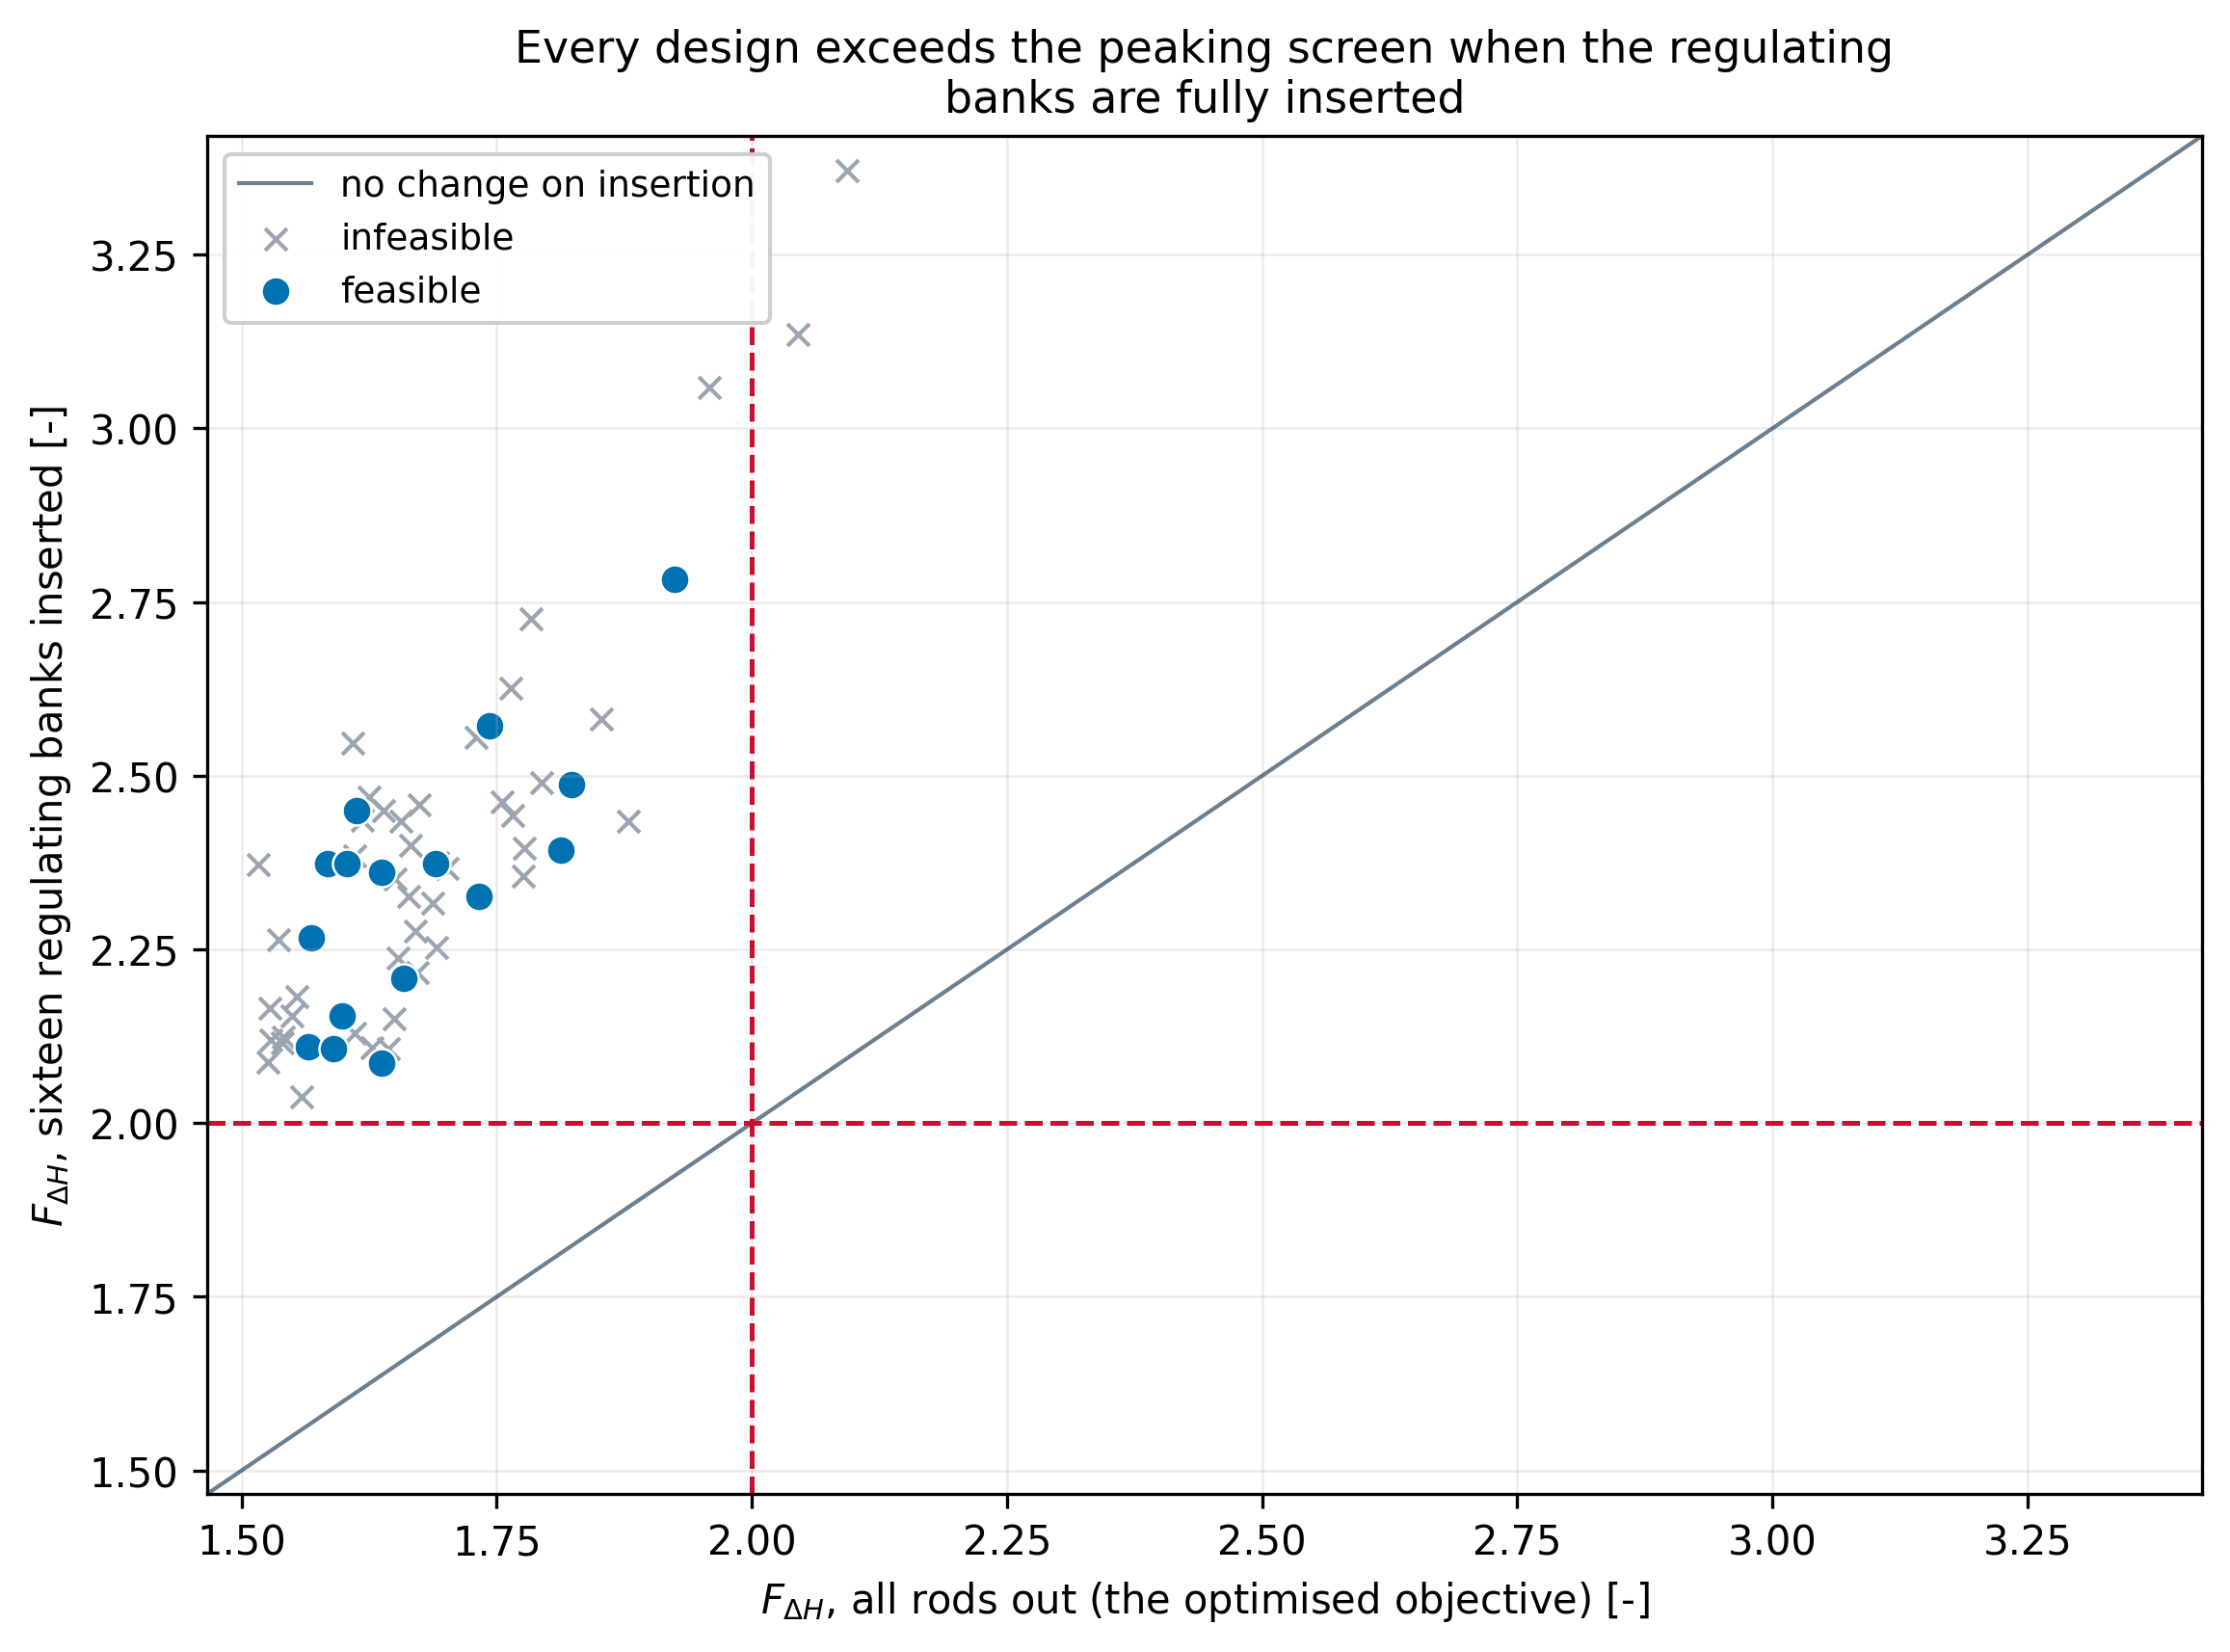
\includegraphics[width=0.85\linewidth]{images/c7_rodded_peaking}
  \caption{Radial peaking with all rods out, the optimised objective,
  against the same quantity with the sixteen regulating banks inserted.
  Every design lies above the screening bound of 2.0 in the rodded
  configuration.}
  \label{fig:c7-rodded}
\end{figure}

With the banks inserted $F_{\Delta H}$ runs from 2.038 to 3.371 with a
mean of 2.375, against 1.516 to 2.093 unrodded. The insertion penalty
ranges from 0.449 to 1.278 and is design dependent, correlating at
$-0.81$ with the outer-zone enrichment over the archive. Every one of
the 60 designs exceeds the screening bound of 2.0 in the rodded
configuration, and the three front designs sit between 2.11 and 2.16.

Two framings are required and neither should be overstated. Sixteen
banks fully inserted is the extreme of the regulating band used here as
a controllability test, not an operating configuration, so the rodded
value is an upper bound on operating peaking rather than an operating
value. Even so, the objective being minimised moves by half a unit or
more when the rods go in, and it moves by a design-dependent amount.
A design selected for low unrodded peaking is not thereby a design
with low rodded peaking. This is recorded as a limitation of the
objective set and as the motivation for the two-level reading of
Campaign 8.

%% AUTHOR: physical interpretation of the negative correlation between
%% the insertion penalty and the outer-zone enrichment.

\subsection{Depletion histories and the statistical error on the cycle length}
\label{sec:res-c7-uncertainty}

The assembly depletion solves are the only transport runs whose output
reaches the campaign log, and the log therefore holds the complete
$k_\infty(B)$ history of every design. Figure~\ref{fig:c7-histories}
reconstructs all 60 histories with the end-of-cycle crossing marked.

\begin{figure}[htbp]
  \centering
  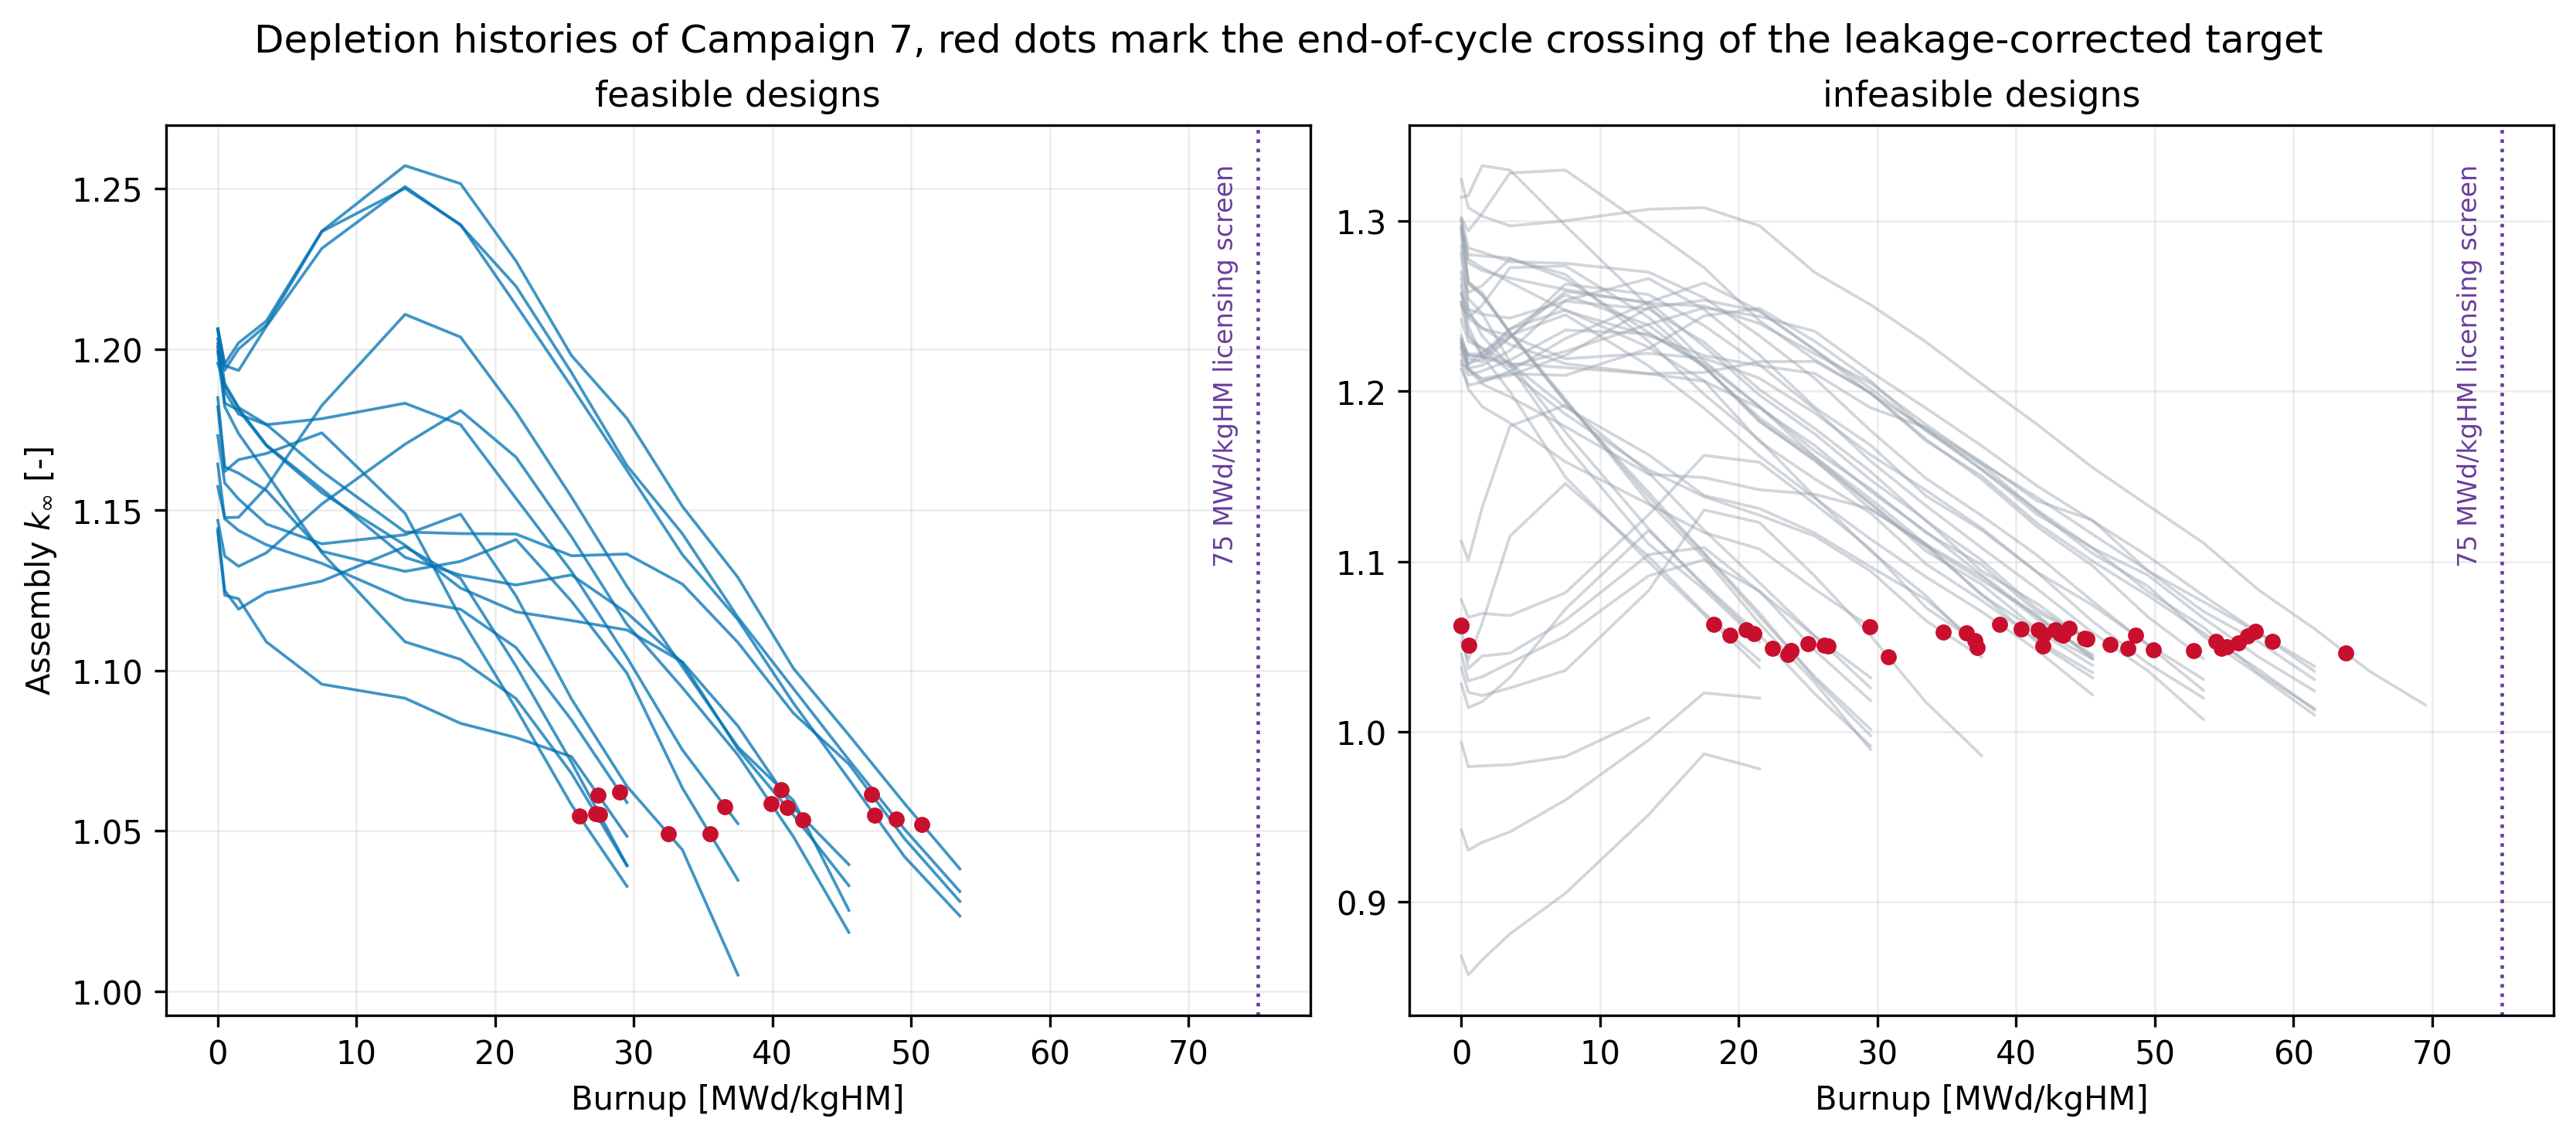
\includegraphics[width=\linewidth]{images/c7_kinf_histories}
  \caption{Assembly infinite multiplication factor against burnup for
  every Campaign 7 design, feasible designs on the left. Red markers
  are the end-of-cycle crossings of the leakage-corrected target. The
  gadolinium burnout maximum is visible between 13 and
  \SI{17}{MWd/kgHM}, and no design approaches the \SI{75}{MWd/kgHM}
  screen.}
  \label{fig:c7-histories}
\end{figure}

The reconstruction was validated against the archive. Taking the last
descending crossing of the target reproduces the stored end-of-cycle
burnup of all 57 crossing designs to within \SI{0.0011}{MWd/kgHM}. The
last crossing is the correct rule because the gadolinium burnout makes
the early history non-monotonic. The three designs without a crossing
are the two subcritical cores at zero cycle length and one design
ending at 55 EFPD.

Three facts follow from the figure. The gadolinium hump raises
$k_\infty$ by up to 0.06 before the decline. The highest end-of-cycle
burnup in the campaign is \SI{63.8}{MWd/kgHM}, so the
\SI{75}{MWd/kgHM} discharge screen of Section~\ref{sec:meth-atf} is
inactive and no design is censored, unlike Campaign 6. And the local
slope at end of cycle is steep, which governs the statistical error on
the cycle length.

The Monte Carlo error on the cycle length is obtained by propagating
the uncertainties of the two transport states that bracket the
crossing.

\begin{equation}
\sigma_B^2 = \left(\frac{\Delta B\,(k_\mathrm{t} - k_{j+1})}{(k_j - k_{j+1})^2}\right)^2 \sigma_{k_j}^2
+ \left(\frac{\Delta B\,(k_j - k_\mathrm{t})}{(k_j - k_{j+1})^2}\right)^2 \sigma_{k_{j+1}}^2
\label{eq:sigma-beoc}
\end{equation}

\noindent where the symbols have the following meaning.

\begin{itemize}
  \item $\sigma_B$ is the statistical uncertainty of the end-of-cycle
        burnup, in MWd/kgHM.

  \item $\Delta B$ is the burnup step between the two bracketing
        states, in MWd/kgHM.

  \item $k_j$ and $k_{j+1}$ are the infinite multiplication factors at
        the states before and after the crossing, dimensionless.

  \item $k_\mathrm{t}$ is the leakage-corrected target, dimensionless,
        treated as exact.

  \item $\sigma_{k_j}$ and $\sigma_{k_{j+1}}$ are the reported Monte
        Carlo standard deviations of the two states, dimensionless.
\end{itemize}

The cycle length follows from the specific power.

\begin{equation}
\sigma_\mathrm{EFPD} = \frac{1000\,\sigma_B}{P_\mathrm{sp}}
\label{eq:sigma-efpd}
\end{equation}

\noindent where the symbols have the following meaning.

\begin{itemize}
  \item $\sigma_\mathrm{EFPD}$ is the statistical uncertainty of the
        cycle length, in effective full power days.

  \item $P_\mathrm{sp}$ is the specific power of the core,
        \SI{9.98}{W/gHM}.
\end{itemize}

\begin{figure}[htbp]
  \centering
  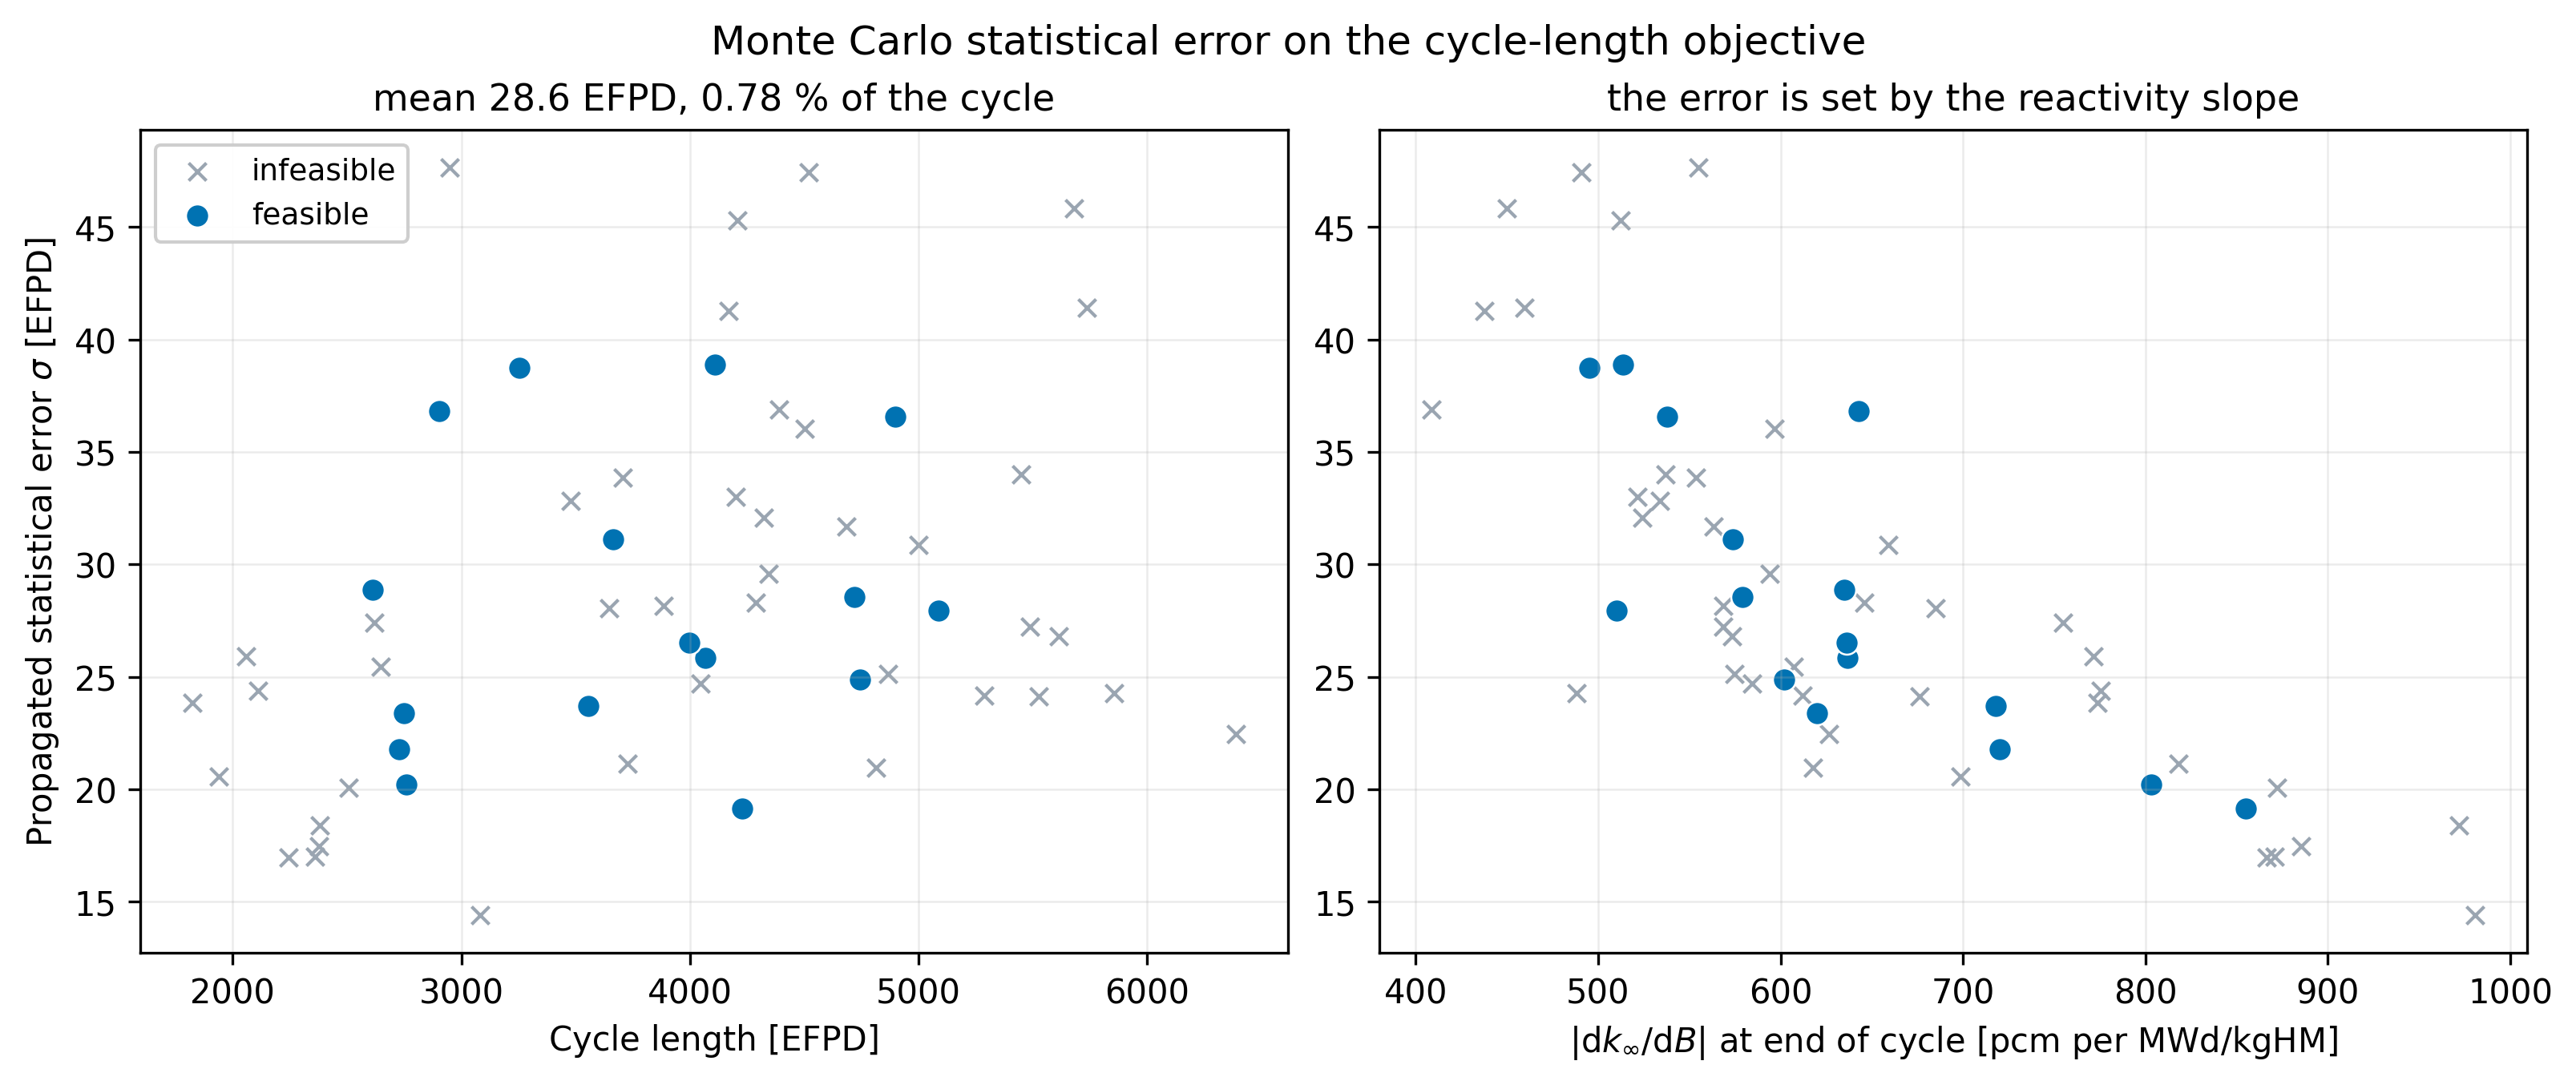
\includegraphics[width=\linewidth]{images/c7_cycle_uncertainty}
  \caption{Propagated Monte Carlo error on the cycle length against the
  cycle length and against the reactivity slope at end of cycle. The
  error is set by the slope, not by the length of the cycle.}
  \label{fig:c7-uncertainty}
\end{figure}

Table~\ref{tab:c7-uncertainty} summarises the result and
Figure~\ref{fig:c7-uncertainty} shows it. The slope at end of cycle
lies between 409 and \SI{981}{pcm} per MWd/kgHM with a median of 607.
The resulting error has a mean of 28.6 EFPD, \SI{0.78}{\%} of the
cycle, and a worst case of 47.7 EFPD, \SI{1.62}{\%}. On the six front
designs it is 25 to 37 EFPD. The smallest gap between adjacent front
designs is 154 EFPD, about five standard deviations, so the ordering of
the front in cycle length is statistically resolved.

\begin{table}[htbp]
  \centering
  \caption{Statistical error on the cycle length over the 57 designs
  with a resolved end-of-cycle crossing.}
  \label{tab:c7-uncertainty}
  \begin{tabular}{lccc}
    \toprule
    Quantity & Minimum & Median & Maximum \\
    \midrule
    Slope at end of cycle [pcm per MWd/kgHM] & 409 & 607 & 981 \\
    Bracketing sigma on $k_\infty$ [pcm]     & 178 & 218 & 274 \\
    $\sigma_\mathrm{EFPD}$ [d]               & 14.4 & 27.2 & 47.7 \\
    $\sigma_\mathrm{EFPD}$ as a fraction of the cycle [\%] & 0.35 & 0.74 & 1.62 \\
    \bottomrule
  \end{tabular}
\end{table}

The peaking axis is the opposite case. The front designs are separated
by 0.003 to 0.036 in $F_{\Delta H}$, the entropy study of
Section~\ref{sec:res-c6} bounded the systematic shift at $\pm 0.02$,
and no statistical error on the core peaking tally has been measured.
The ordering of the front in peaking is therefore not resolved, and
designs 59, 57 and 55 at 1.525, 1.528 and 1.529 must be treated as
indistinguishable until the tally errors are read from the statepoints.

\openpoint{Measure $\sigma(F_{\Delta H})$ from the per-bin relative
errors of the core mesh tally on the six front designs, or by seed
replicates, before any ordering claim on the peaking axis is made.}

\subsection{Cost and instrumentation}
\label{sec:res-c7-cost}

The campaign cost \SI{56965}{s} of wall time, \SI{949}{s} per
evaluation, against \SI{840}{s} in Campaign 6. The difference is the
control solve. Two instrumentation defects were found while reading
the archive, and both are recorded because they affect numbers reported
elsewhere in this chapter.

\begin{enumerate}
  \item The per-evaluation cost stored in the archive excludes the
        control solve, because that solve is invoked after the three
        timers close. Over the campaign the control solves are
        \SI{11}{\%} of the true cost and \SI{12.6}{\%} of the reported
        cost. The wall-clock figure of the block log is correct and is
        the one quoted above. The evaluator is corrected from Campaign
        8 (Section~\ref{sec:meth-cost}).

  \item The per-case parser of the run log never matched a single case
        line of any campaign, because the censoring marker inserted
        after the cycle length was not anticipated by its regular
        expression. The failure was silent, and every per-case table
        the parser produced before the correction was empty. No number
        in this chapter depends on that table, since all per-design
        quantities are read from the archive.
\end{enumerate}

\subsection{Limitations and what carries forward}
\label{sec:res-c7-limits}

Four limitations bound the claims of this section.

\begin{enumerate}
  \item Four designs, 10, 32, 41 and 43, reached the active batches
        with the Shannon entropy of the fission source not yet
        converged, the worst at 105 of 60 inactive batches. None is on
        either front. Their eigenvalues and peaking values carry an
        unquantified bias, are retained in the archive statistics of
        this section with that caveat, and are excluded from any
        candidate list.

  \item Twenty-five of the 60 designs have a pitch below
        \SI{1.2242}{cm}, twice the guide-tube outer radius. Below that
        value the lattice clips the guide-tube wall at the cell
        boundary silently, replacing up to \SI{27}{\%} of the wall
        cross-section by moderator at the box minimum of
        \SI{1.150}{cm}. Designs 57 and 59, the two lowest-peaking
        designs of the control-screen front, are both in the affected
        band. The same defect reaches back to every earlier campaign
        design at pitches below \SI{1.2242}{cm}, including the
        Campaign 4 infill designs pinned at the box minimum and the
        Campaign 6 discharge-screen champion at \SI{1.150}{cm}. Fixing
        the pitch at \SI{1.26}{cm} in Campaign 8 removes the defect
        prospectively, and a caveat is added to the affected results.

  \item The statistical error on the peaking objective is not
        measured, as stated above.

  \item Every cycle length in this campaign, as in all earlier ones, is
        a two-dimensional value. The axial leakage study of
        Section~\ref{sec:meth-lax}, completed after this campaign,
        measured the axial correction at \num{1.0282} to \num{1.0298}
        on six Campaign 6 designs, about \SI{3000}{pcm} of reactivity,
        which at the end-of-cycle slopes measured here corresponds to
        roughly 450 to 500 EFPD. Campaign 7 cycle lengths are therefore
        overstated by that amount relative to a finite-height core,
        uniformly across the archive, and the ordering of the front is
        unaffected. Campaign 8 carries the correction inside the
        end-of-cycle target from the start.
\end{enumerate}

What carries forward is the constraint architecture. The measured
control screen replaces the derived ceiling as the reactivity
constraint that does the work, a second reading with only the first two
banks inserted is added and recorded, the axial factor enters the
target, the acquisition settings of Campaign 6 are restored explicitly,
and the pitch is fixed at the value that both closes the geometric
defect and matches the reference fuel design. Section~\ref{sec:res-c8}
states the campaign built on those decisions.
 at that point.
%
%  Figures: copy the eight PDF files of c7_analysis_60/ into images/.
%    c7_pareto_60, c7_ctrl_screen, c7_rod_worth, c7_rodded_peaking,
%    c7_kinf_histories, c7_cycle_uncertainty, c7_infill_diversity,
%    c7_vars_influence
%
%  Labels defined here: sec:res-c7, sec:res-c7-basis, sec:res-c7-blocks,
%  sec:res-c7-screens, sec:res-c7-worth, sec:res-c7-rodded,
%  sec:res-c7-uncertainty, sec:res-c7-cost, sec:res-c7-limits,
%  tab:c7-blocks, tab:c7-front, tab:c7-nesting, tab:c7-uncertainty,
%  fig:c7-diversity, fig:c7-screens, fig:c7-pareto, fig:c7-worth,
%  fig:c7-influence, fig:c7-rodded, fig:c7-histories, fig:c7-uncertainty,
%  eq:g-ctrl, eq:k-implied, eq:bank-worth, eq:sigma-beoc, eq:sigma-efpd
%
%  Labels used from elsewhere: sec:meth-ctrl, sec:meth-ktarget,
%  sec:meth-acq, sec:res-c6, sec:res-c6-blocks, tab:fidelity,
%  sec:meth-lax, sec:res-c8, sec:meth-cost. Define sec:meth-ctrl,
%  sec:meth-lax and sec:meth-cost with methodology_c78_additions.tex.
%
%  Style: short paragraphs, no semicolons, no em dashes, every displayed
%  formula followed by a term list with units, enumerations as lists.
% =====================================================================

\section{Campaign 7: the controllability screen}
\label{sec:res-c7}

Campaign 6 closed with a front whose long-cycle end rode the
reactivity ceiling, and with the observation that the ceiling of 1.35
proxied controllable excess reactivity without a rod model. Campaign 7
replaces the proxy by a measurement. Every evaluation now solves the
beginning-of-life core a second time with the sixteen regulating-bank
control rod assemblies inserted, and the resulting eigenvalue enters the
constraint set directly. The campaign ran 60 evaluations on the AWS
instance in \SI{15.82}{h}, and every one of them completed without
error.

\subsection{The one change and its two consequences}
\label{sec:res-c7-basis}

The constraint added is the controllability screen of
Section~\ref{sec:meth-ctrl}.

\begin{equation}
g_\mathrm{ctrl}(\mathbf{x}) = k_\mathrm{ARI}(\mathbf{x}) - (1 - \Delta\rho_\mathrm{op}) \le 0
\label{eq:g-ctrl}
\end{equation}

\noindent where the symbols have the following meaning.

\begin{itemize}
  \item $k_\mathrm{ARI}$ is the effective multiplication factor of the
        32-assembly core at beginning of life with all sixteen
        regulating-bank assemblies inserted and the shutdown banks
        withdrawn, dimensionless.

  \item $\Delta\rho_\mathrm{op}$ is the operating subcriticality margin
        demanded of the regulating banks, \num{0.01} in units of $k$,
        that is \SI{1000}{pcm}.

  \item $\mathbf{x}$ is the design vector.
\end{itemize}

Two settings changed with it. The reactivity ceiling was lowered from
1.35 to 1.126, a value derived before the campaign from the smallest
regulating-bank worth measured on eight Campaign 6 designs, and the
enrichment cap was lowered to \SI{12}{wt\%} on the as-built peripheral
ring, giving a search box of 3.0 to \SI{10.43}{wt\%}. Both were
intended as consequences of the controllability requirement rather than
as independent changes, and the campaign tests whether they were
consistent with the measurement they were meant to anticipate.

\subsection{Design of experiments and the three infill blocks}
\label{sec:res-c7-blocks}

The campaign ran a design of experiments of 42 followed by three infill
blocks of six. Table~\ref{tab:c7-blocks} records the outcome of each
block and Figure~\ref{fig:c7-diversity} its diversity, measured as the
spread of each design variable within the block as a fraction of the
range spanned by the whole archive.

\begin{table}[htbp]
  \centering
  \caption{Campaign 7 blocks. The hypervolume is the frozen-reference
  value written at each block boundary. Spread is the within-block
  range of each variable as a fraction of the archive range, listed
  for the four non-geometric variables.}
  \label{tab:c7-blocks}
  \begin{tabular}{lccll}
    \toprule
    Block & Designs & Feasible & Hypervolume & Spread in $e_\mathrm{in}$, $e_\mathrm{out}$, $w_\mathrm{Gd}$, $n_\mathrm{Gd}$ \\
    \midrule
    DOE      & 42 & 13 & 773.7 & 0.98 to 1.00 \\
    Infill 1 &  6 &  0 & 773.7 & 0.000 to 0.002 \\
    Infill 2 &  6 &  3 & 996.5 & 0.07 to 0.29 \\
    Infill 3 &  6 &  0 & 996.5 & 0.015 to 0.13 \\
    \bottomrule
  \end{tabular}
\end{table}

\begin{figure}[htbp]
  \centering
  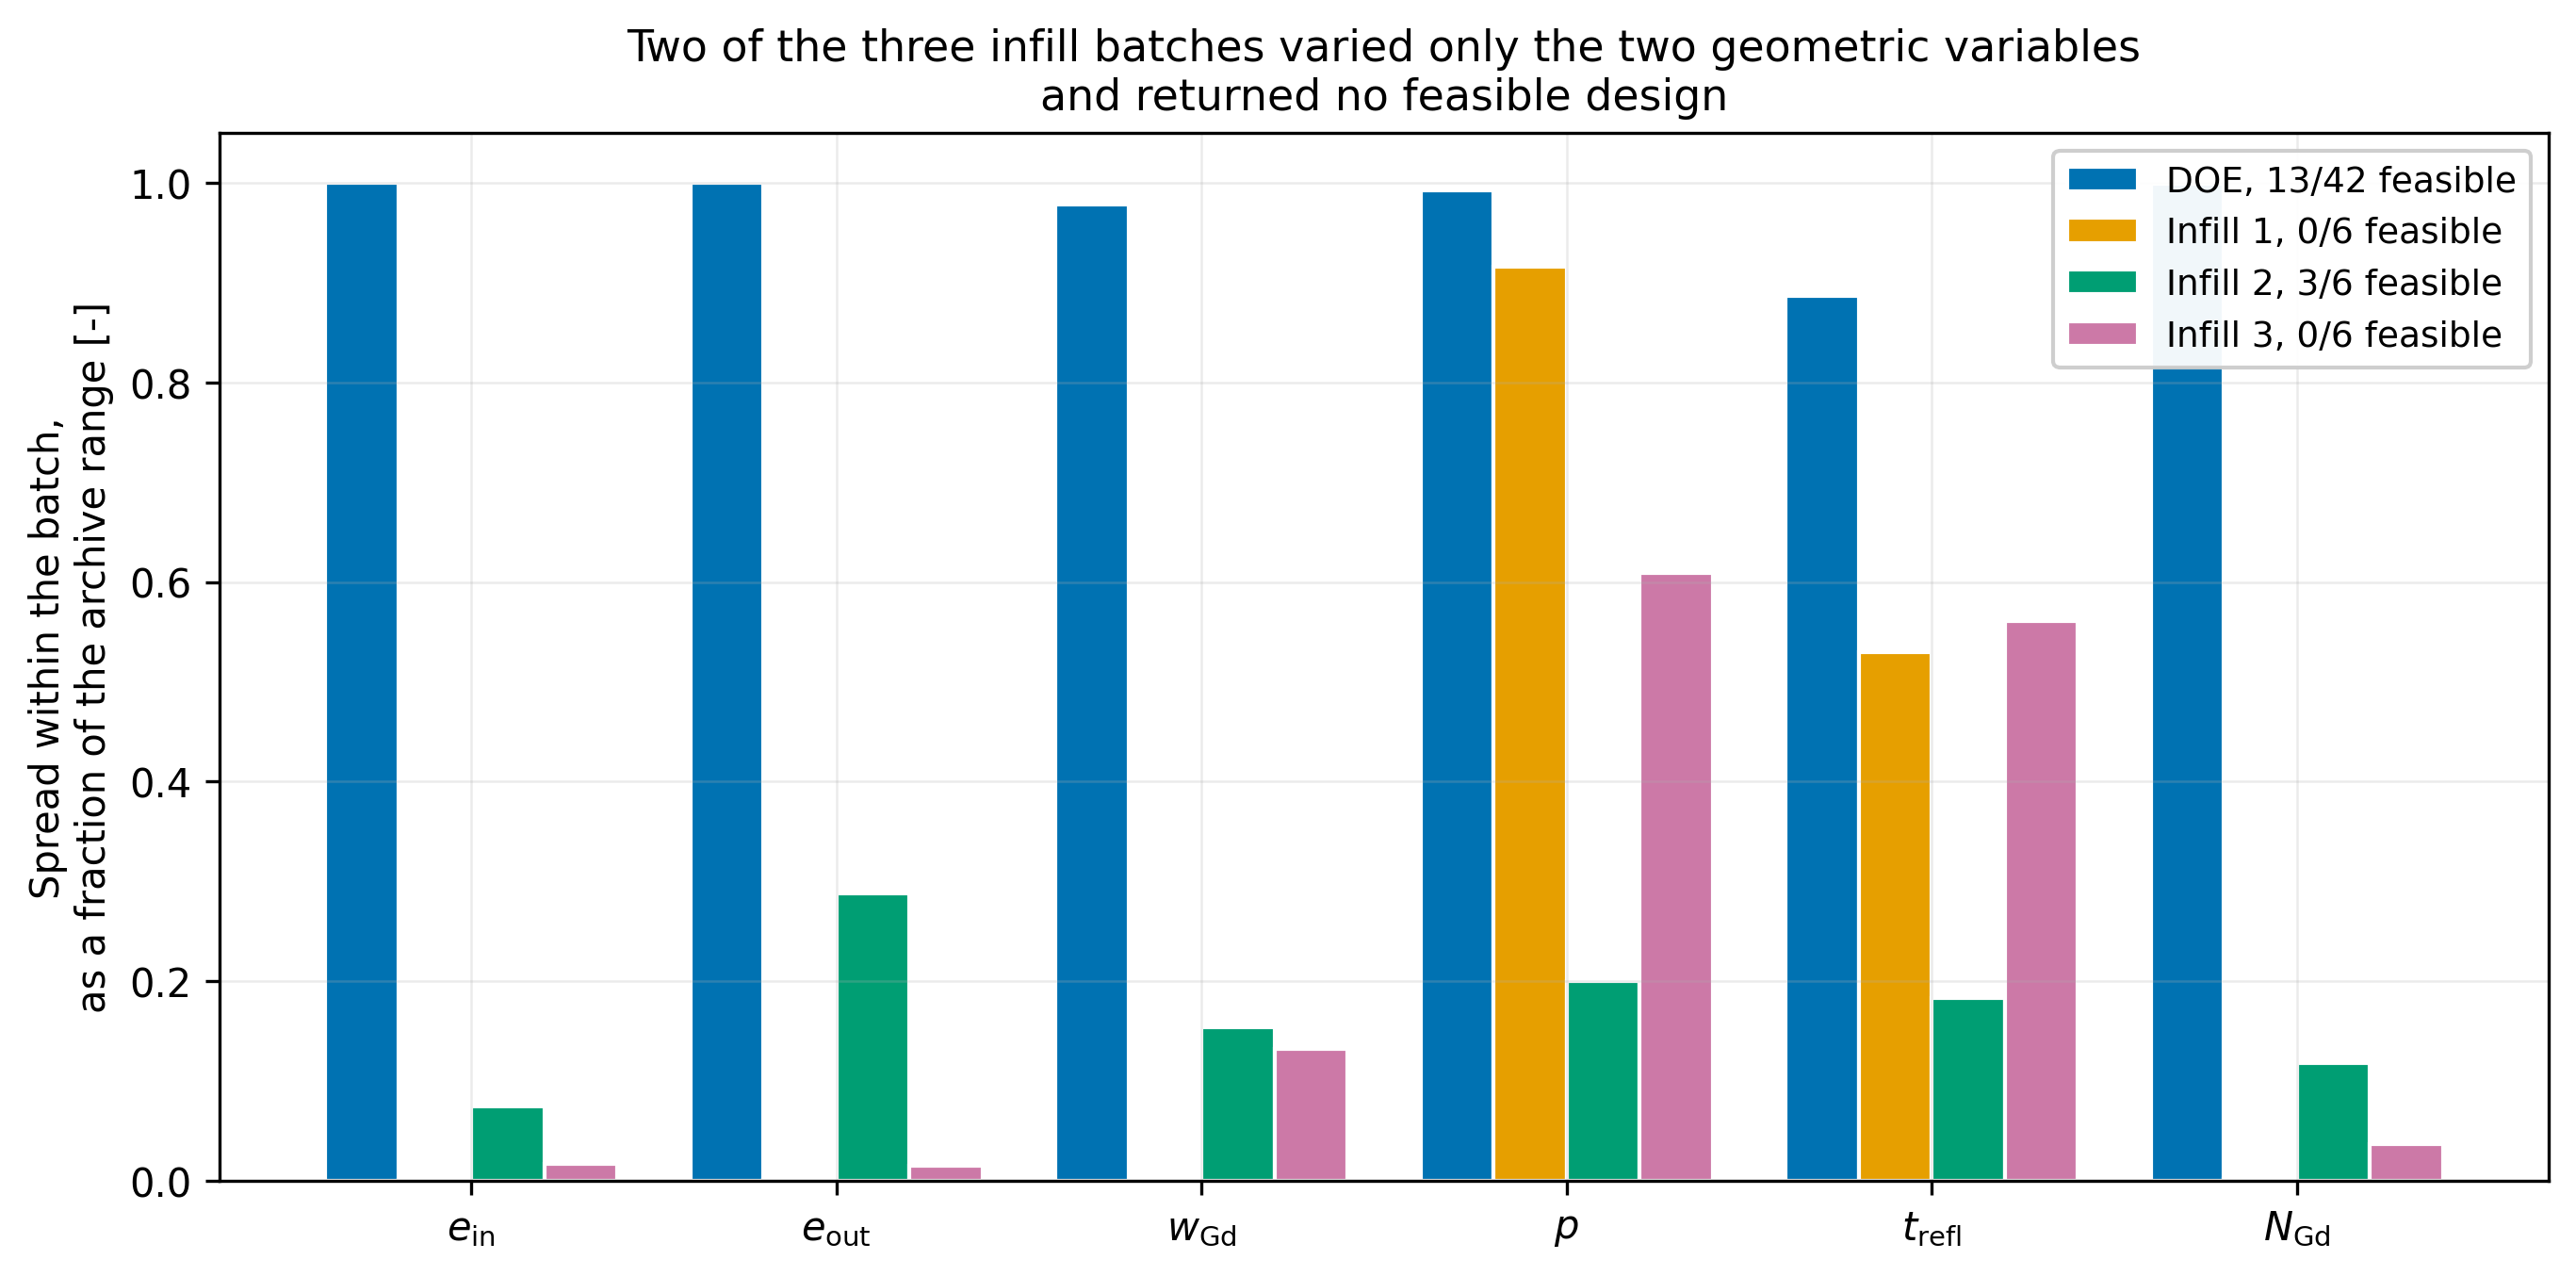
\includegraphics[width=\linewidth]{images/c7_infill_diversity}
  \caption{Within-block spread of each design variable, as a fraction
  of the archive range. Infill blocks 1 and 3 vary only the pitch and
  the reflector thickness, and neither returned a feasible design.}
  \label{fig:c7-diversity}
\end{figure}

Two of the three infill blocks collapsed. In block 1 the six designs
share one enrichment pair, \num{5.09} and \SI{4.04}{wt\%}, exactly zero
gadolinia and 24 poisoned pins, and differ only in pitch and reflector
thickness. In block 3 the same pattern recurs at \num{8.13} and
\SI{7.33}{wt\%} with 32 pins. All twelve designs of the two blocks
failed the reactivity ceiling.

The cause is a configuration regression, not a new defect. The
acquisition ran with a minimum separation of 0.05 and a feasibility
margin of 1.0 standard deviation, the default values of the launcher,
where Campaign 6 had established 0.14 and 1.5 in
Section~\ref{sec:res-c6-blocks}. The two collapsed blocks satisfied the
separation rule as coded, with pairwise separations of 0.059 to 0.089,
because the rule averages over all six variables and two of them
supplied the whole distance. A per-variable minimum spread would have
rejected both batches.

The consequence for the convergence record is that the flat
hypervolume of block 3 is not a stopping signal. Under the Campaign 6
rule a zero gain counts toward stopping only when the acquisition is
functioning, and block 3 demonstrably was not. The campaign therefore
ends with an unconverged front, and its value lies in the constraint
measurements rather than in the front itself.

\subsection{Feasibility and the nesting of the two screens}
\label{sec:res-c7-screens}

Of the 60 designs, 16 are feasible against all six constraints, a
fraction of \SI{26.7}{\%} against \SI{67}{\%} in the Campaign 6 design
of experiments. Table~\ref{tab:c7-nesting} gives the constraint census.
No design fails the enrichment or the geometric constraint, two fail
the peaking limit, nine fall below the reactivity floor, 34 exceed the
ceiling and 20 fail the controllability screen.

\begin{table}[htbp]
  \centering
  \caption{Constraint census of Campaign 7 and the joint activity of
  the two reactivity screens. Every design that fails the
  controllability screen also fails the derived ceiling, and fourteen
  designs fail the ceiling while passing the controllability screen.}
  \label{tab:c7-nesting}
  \begin{tabular}{lc}
    \toprule
    Outcome & Designs \\
    \midrule
    Fail $g_{k\max}$ at 1.126                      & 34 \\
    Fail $g_\mathrm{ctrl}$                         & 20 \\
    Fail $g_\mathrm{ctrl}$ and pass $g_{k\max}$    &  0 \\
    Fail $g_{k\max}$ and pass $g_\mathrm{ctrl}$    & 14 \\
    Pass every constraint except $g_{k\max}$       & 14 \\
    Feasible on all six                            & 16 \\
    \bottomrule
  \end{tabular}
\end{table}

\begin{figure}[htbp]
  \centering
  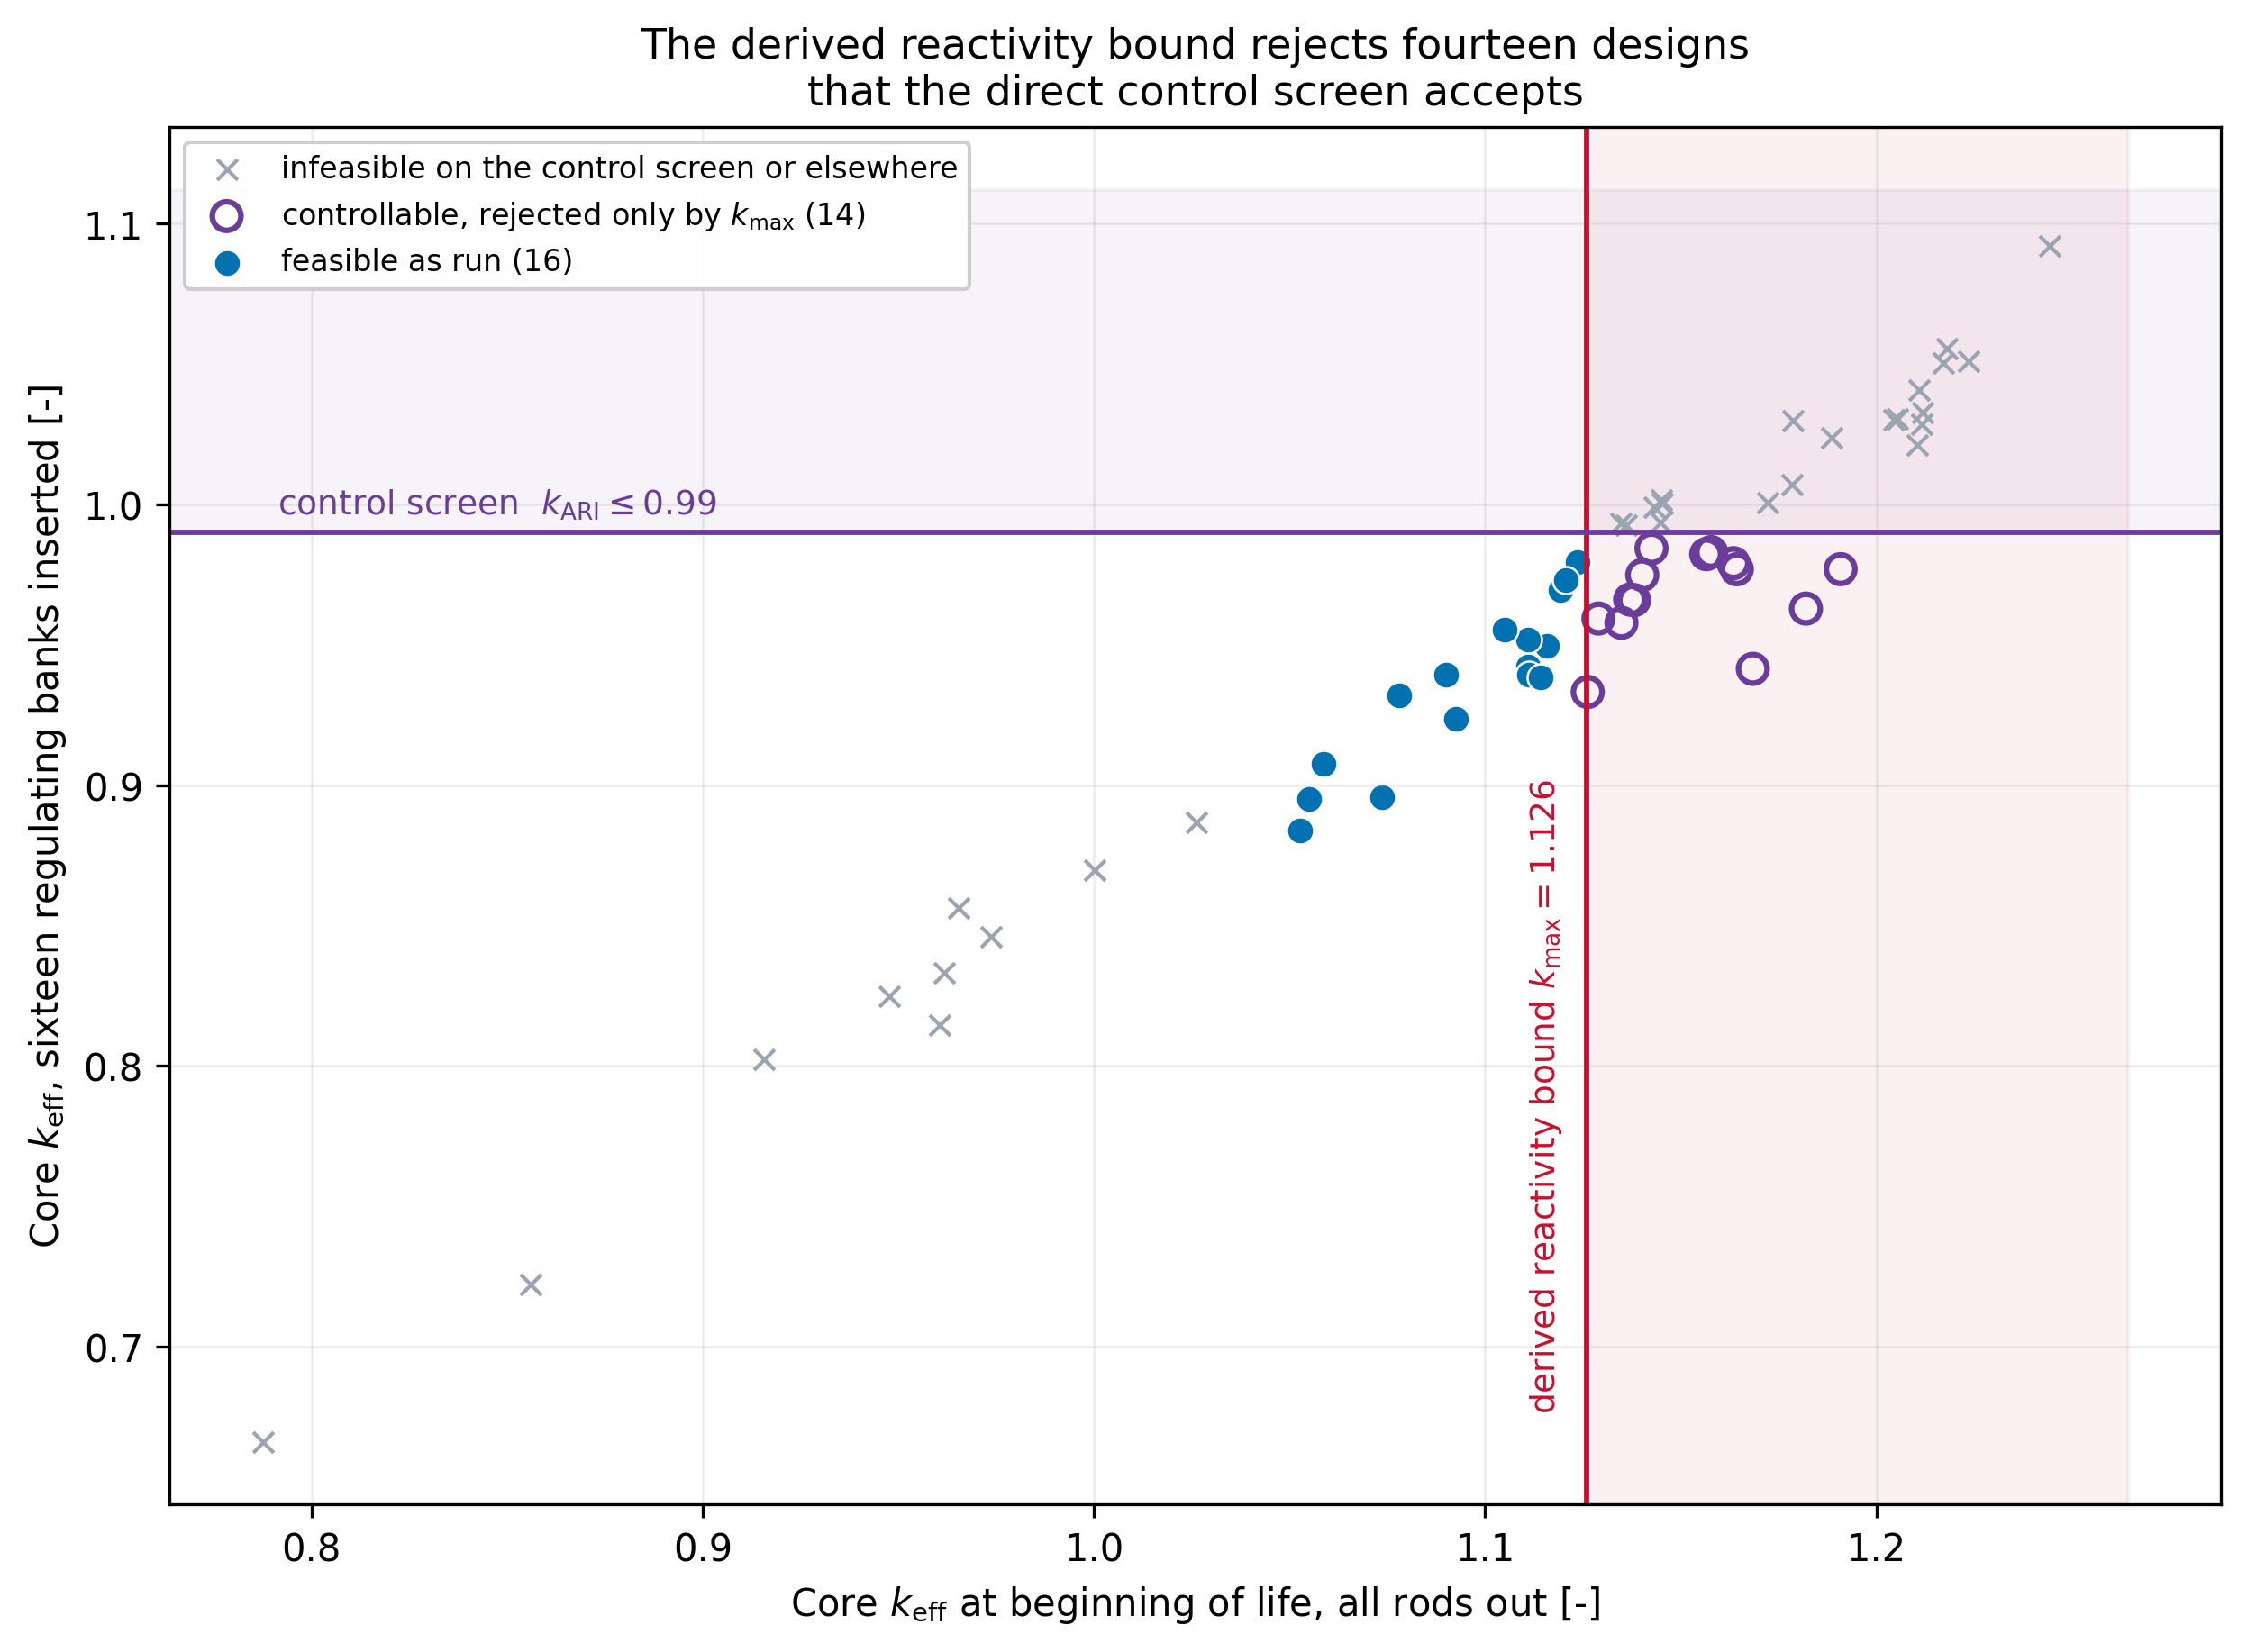
\includegraphics[width=0.9\linewidth]{images/c7_ctrl_screen}
  \caption{The two reactivity screens of Campaign 7 in the plane of
  the unrodded and the all-regulating-banks-in core eigenvalues. The
  derived ceiling at 1.126 rejects fourteen designs, marked by open
  circles, that the directly measured control screen accepts.}
  \label{fig:c7-screens}
\end{figure}

The two screens are nested. Not one design in the archive fails the
control screen without also failing the derived ceiling, and fourteen
designs fail the ceiling while their own measured bank worth shows them
controllable at the stated margin. Figure~\ref{fig:c7-screens} shows
the nesting directly. The ceiling of 1.126 therefore did no work that
the measurement did not do, and it discarded fourteen evaluations that
the measurement would have kept.

The derivation explains why. The eight Campaign 6 designs from which
1.126 was obtained had worths between \num{12174} and
\SI{12718}{pcm}, a spread of four per cent. The 60 designs of this
campaign span \num{10936} to \SI{22699}{pcm}, a factor of two. Eight
near-identical designs under-sampled the variability by an order of
magnitude, and the resulting bound is at once too tight where it
matters and not conservative in general. Restricted to the 22 designs
with an unrodded eigenvalue between 1.09 and 1.17, the smallest
measured worth of \SI{14126}{pcm} implies a ceiling of 1.151, while the
smallest worth in the whole archive implies 1.110.

The front reflects the same fact. As run, the feasible non-dominated set
holds three designs, all from infill block 2. With the derived ceiling
removed and the measured control screen retained, the feasible set grows
from 16 to 30 designs, the front doubles to six, the peaking floor moves
from 1.565 to 1.525, and the hypervolume against the frozen reference
rises from 996.5 to 1054.1, a gain of \SI{5.8}{\%}. Three of the six
designs come from infill block 3, the block that under the ceiling
contributed nothing. Table~\ref{tab:c7-front} lists both fronts and
Figure~\ref{fig:c7-pareto} places them in the objective plane.

\begin{table}[htbp]
  \centering
  \small
  \caption{The Campaign 7 front under the two screening rules. Designs
  48, 53 and 49 form the front as run. All six form the front when the
  measured control screen alone governs reactivity. Bank worth is the
  difference between the unrodded and the all-banks-in eigenvalues.}
  \label{tab:c7-front}
  \begin{tabular}{ccccccccccc}
    \toprule
    Design & EFPD & $F_{\Delta H}$ & $e_\mathrm{in}$ & $e_\mathrm{out}$ & $w_\mathrm{Gd}$ & $p$ & $t_\mathrm{refl}$ & $n_\mathrm{Gd}$ & $k_\mathrm{eff}^\mathrm{core}$ & worth \\
           & [d] & [-] & [wt\%] & [wt\%] & [wt\%] & [cm] & [cm] & [-] & [-] & [pcm] \\
    \midrule
    59 & 3886 & 1.525 & 8.13 & 7.33 & 1.10 & 1.150 & 19.49 & 32 & 1.135 & 17699 \\
    57 & 4045 & 1.528 & 8.13 & 7.33 & 1.21 & 1.176 & 17.87 & 32 & 1.137 & 17094 \\
    55 & 4502 & 1.529 & 8.14 & 7.34 & 1.10 & 1.238 & 14.09 & 32 & 1.143 & 15815 \\
    48 & 4745 & 1.565 & 8.71 & 7.80 & 1.93 & 1.237 & 14.06 & 40 & 1.119 & 14970 \\
    53 & 4899 & 1.590 & 8.97 & 7.88 & 1.96 & 1.249 & 13.21 & 40 & 1.121 & 14734 \\
    49 & 5087 & 1.598 & 9.19 & 8.30 & 2.13 & 1.267 & 12.29 & 40 & 1.124 & 14416 \\
    \bottomrule
  \end{tabular}
\end{table}

\begin{figure}[htbp]
  \centering
  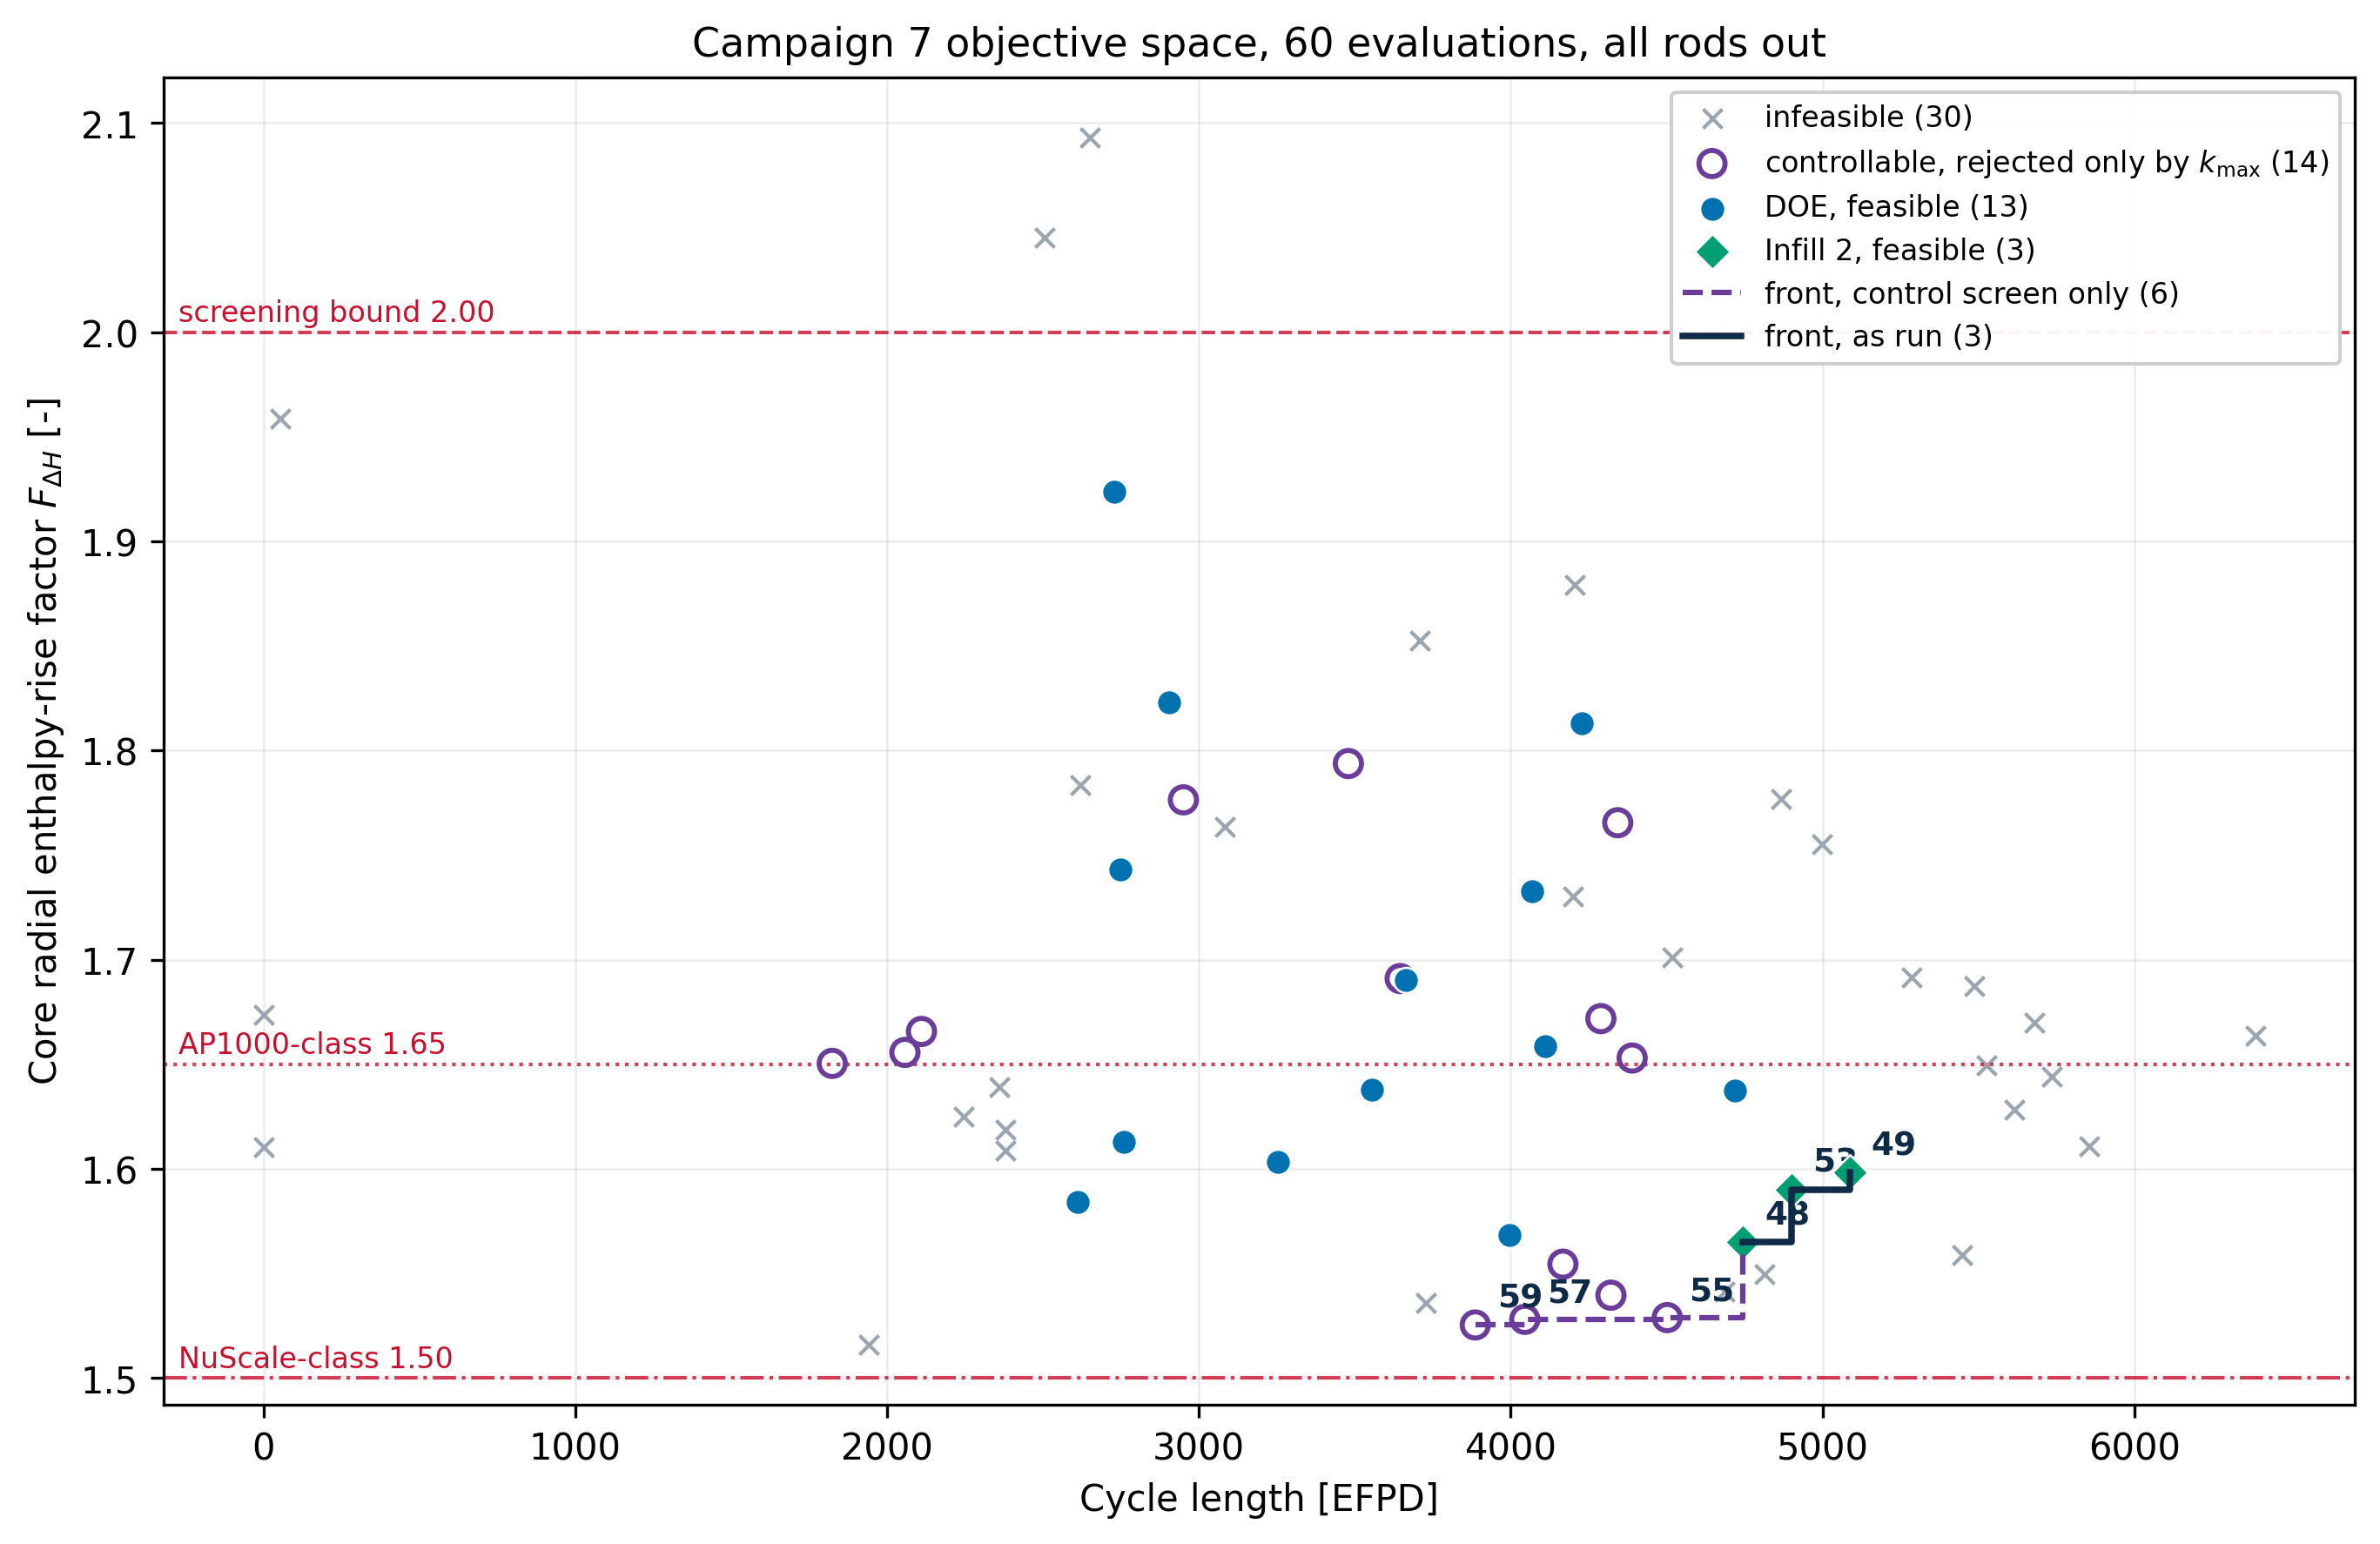
\includegraphics[width=\linewidth]{images/c7_pareto_60}
  \caption{Campaign 7 objective space with all rods out. Filled markers
  are feasible as run, open circles are controllable designs rejected
  only by the derived ceiling. The solid front is the one the campaign
  reported and the dashed front is the one the measured control screen
  supports.}
  \label{fig:c7-pareto}
\end{figure}

Two properties of the front as run deserve stating. Its three designs
sit \num{240} to \SI{680}{pcm} below the ceiling, so the front is a
constraint boundary and not an interior trade. And the cycle lengths
are not comparable with Campaign 6, because the enrichment box is a
different one, and the longest feasible cycle of 5087 EFPD says nothing
about the reactor class that the 9981 EFPD of Campaign 6 did not
already say.

%% AUTHOR: one paragraph on why the low-peaking end of the control-screen
%% front lives at thick reflectors and narrow pitch, and on the physical
%% meaning of a front that doubles when a surrogate bound is removed.

\subsection{Regulating-bank worth and the reason the screens nest}
\label{sec:res-c7-worth}

The worth of the sixteen regulating banks is defined on the two core
solves of every evaluation.

\begin{equation}
\rho_\mathrm{bank}(\mathbf{x}) = k_\mathrm{eff}^\mathrm{core}(\mathbf{x}) - k_\mathrm{ARI}(\mathbf{x})
\label{eq:bank-worth}
\end{equation}

\noindent where the symbols have the following meaning.

\begin{itemize}
  \item $\rho_\mathrm{bank}$ is the bank worth in units of $k$,
        dimensionless, reported in pcm by multiplying by $10^5$.

  \item $k_\mathrm{eff}^\mathrm{core}$ is the unrodded core eigenvalue
        at beginning of life, dimensionless.

  \item $k_\mathrm{ARI}$ is the eigenvalue with all sixteen regulating
        banks inserted, dimensionless.
\end{itemize}

Across the archive the worth ranges from \num{10936} to
\SI{22699}{pcm} with a median of \SI{16510}{pcm}. Figure~\ref{fig:c7-worth}
shows its two strongest drivers and Figure~\ref{fig:c7-influence} the
rank correlations of all six variables with the objectives, the worth
and the rodded peaking.

\begin{figure}[htbp]
  \centering
  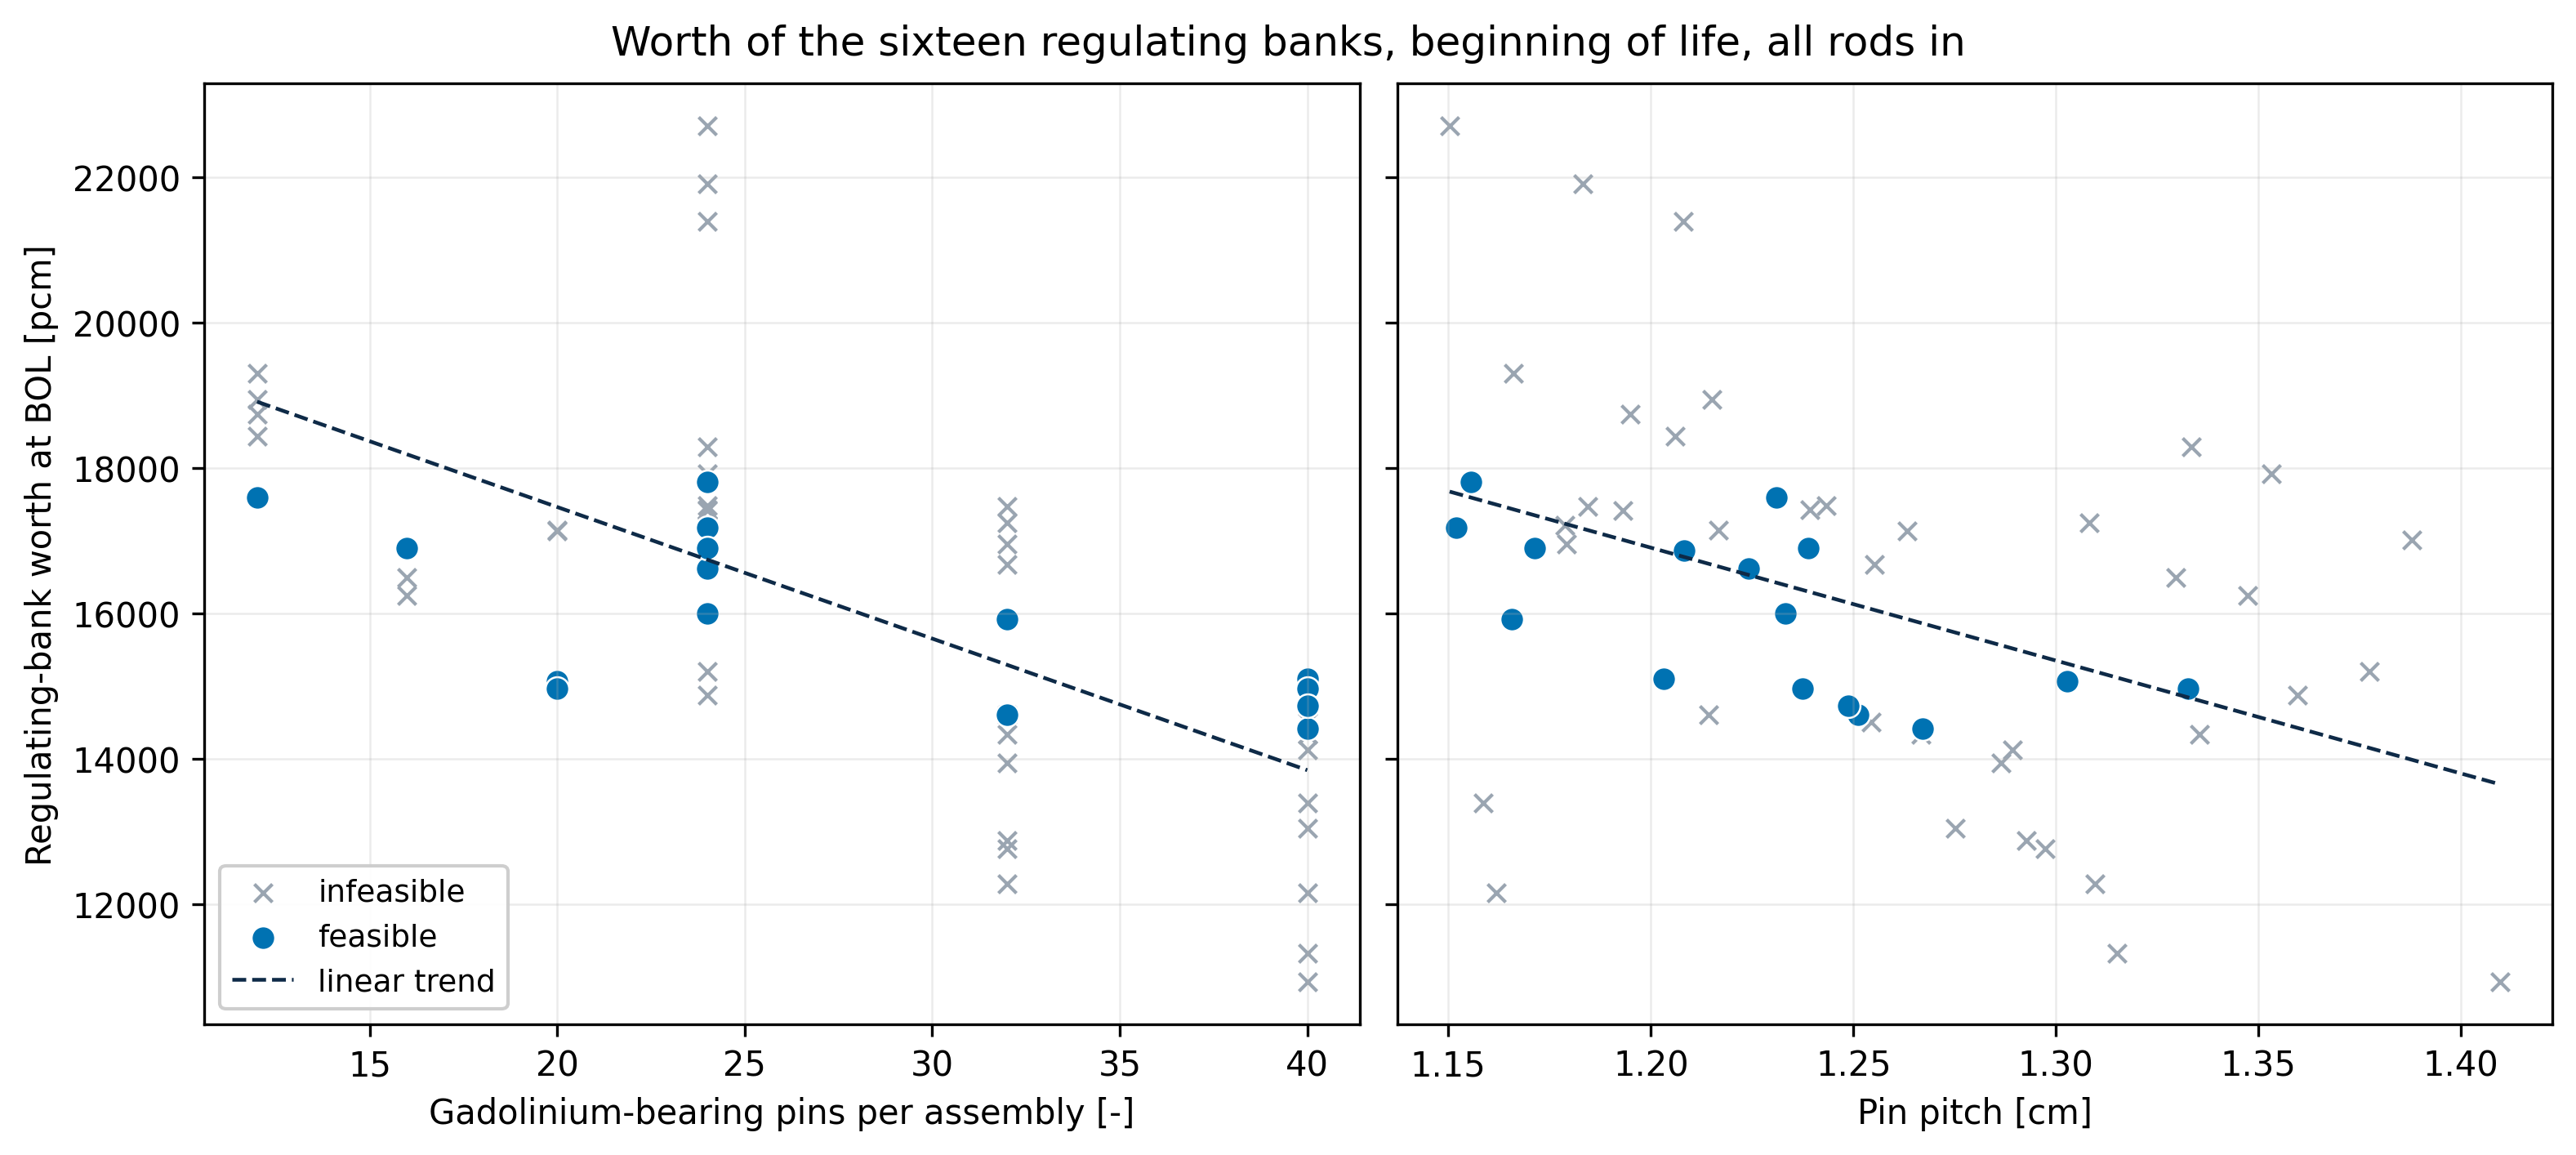
\includegraphics[width=\linewidth]{images/c7_rod_worth}
  \caption{Worth of the sixteen regulating banks against the
  gadolinium pin count and the pin pitch. The dashed lines are
  least-squares trends and serve only as visual guides.}
  \label{fig:c7-worth}
\end{figure}

\begin{figure}[htbp]
  \centering
  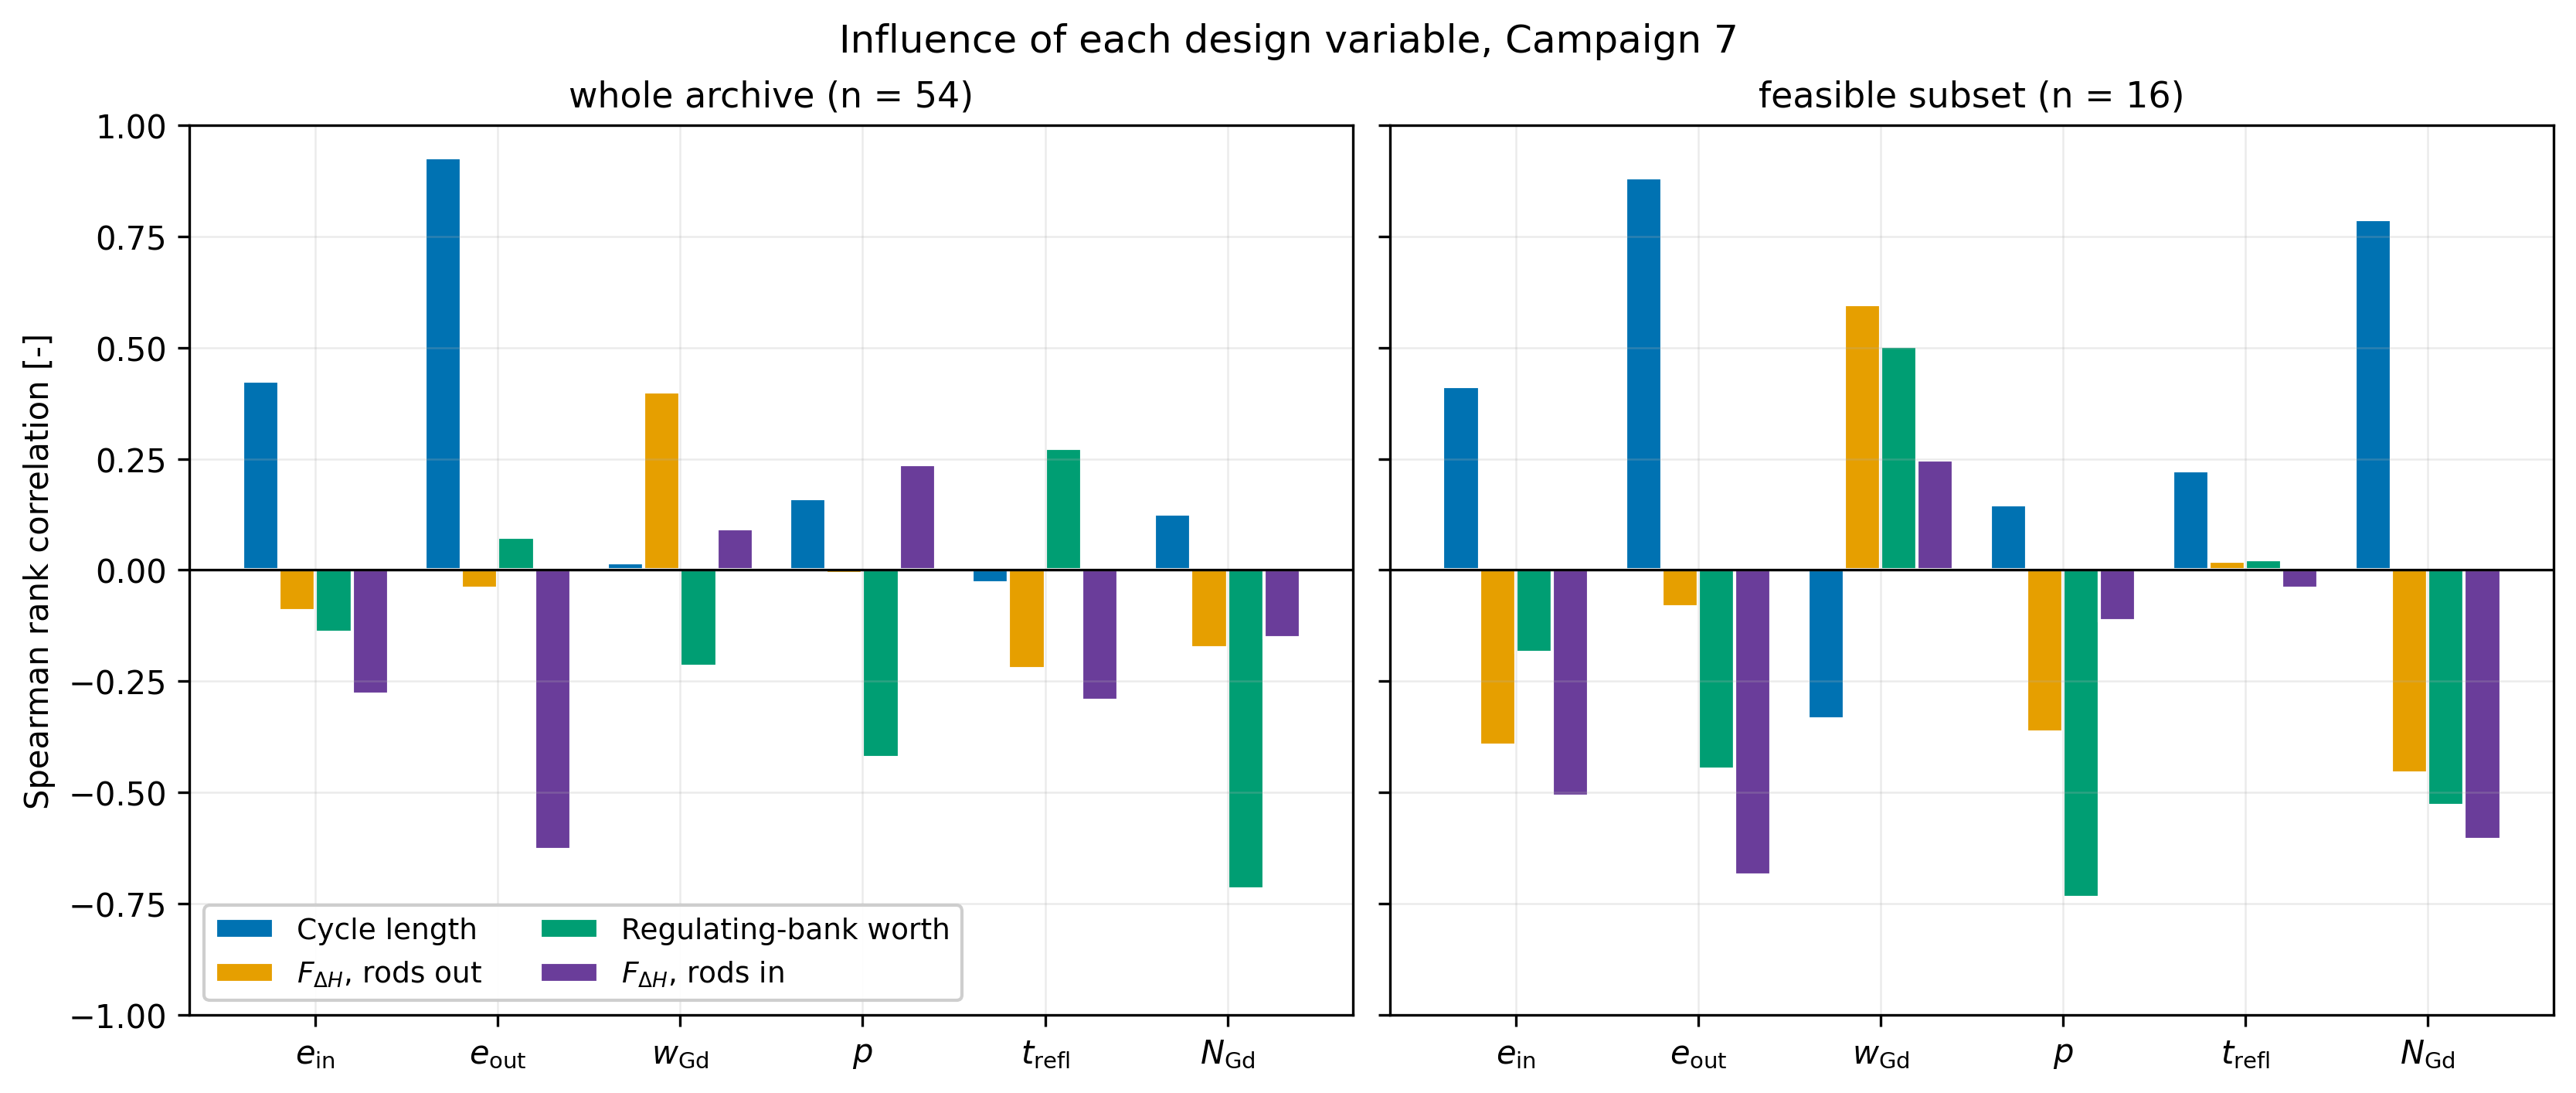
\includegraphics[width=\linewidth]{images/c7_vars_influence}
  \caption{Spearman rank correlation of each design variable with the
  two objectives, the regulating-bank worth and the peaking with the
  banks inserted, over the whole archive and over the feasible subset.}
  \label{fig:c7-influence}
\end{figure}

The worth correlates at $-0.68$ with the gadolinium pin count, at
$-0.45$ with the pitch and at $+0.61$ with the unrodded eigenvalue.
Gadolinium depresses the eigenvalue and the bank worth together, so the
designs with the least worth are the heavily poisoned ones, which are
already far below the ceiling for a different reason. That is why the
two screens nest in this design space, and it is also why the
eight-design derivation of the ceiling looked safe when it was not.
The eight designs were all high-enrichment, forty-pin designs from one
corner of the Campaign 6 front, and their worths were alike because
their poison inventories were alike.

The measurement also settles a question left open since Campaign 4.
The ceiling of 1.35 used in Campaigns 1 to 6 was described as a
screening value not traceable to a primary source. Deriving the
ceiling from the worth of all seven banks, that is all 32 control rod
assemblies, with the same \SI{1000}{pcm} margin gives 1.368. The value
used through six campaigns sits two per cent below the measured
all-bank controllability bound of this core. It is a measured quantity
in retrospect, and the methodology chapter now states it as such,
with the caveat that an all-bank insertion with a \SI{1000}{pcm}
operating margin is not a licensing shutdown margin, which also
requires the highest-worth assembly stuck out and the cold, xenon-free
state.

\subsection{Peaking with the regulating banks inserted}
\label{sec:res-c7-rodded}

The peaking objective is evaluated with all rods out. The same core
solve that measures $k_\mathrm{ARI}$ also yields the radial peaking
with the sixteen banks inserted, and Figure~\ref{fig:c7-rodded} plots
the two against each other.

\begin{figure}[htbp]
  \centering
  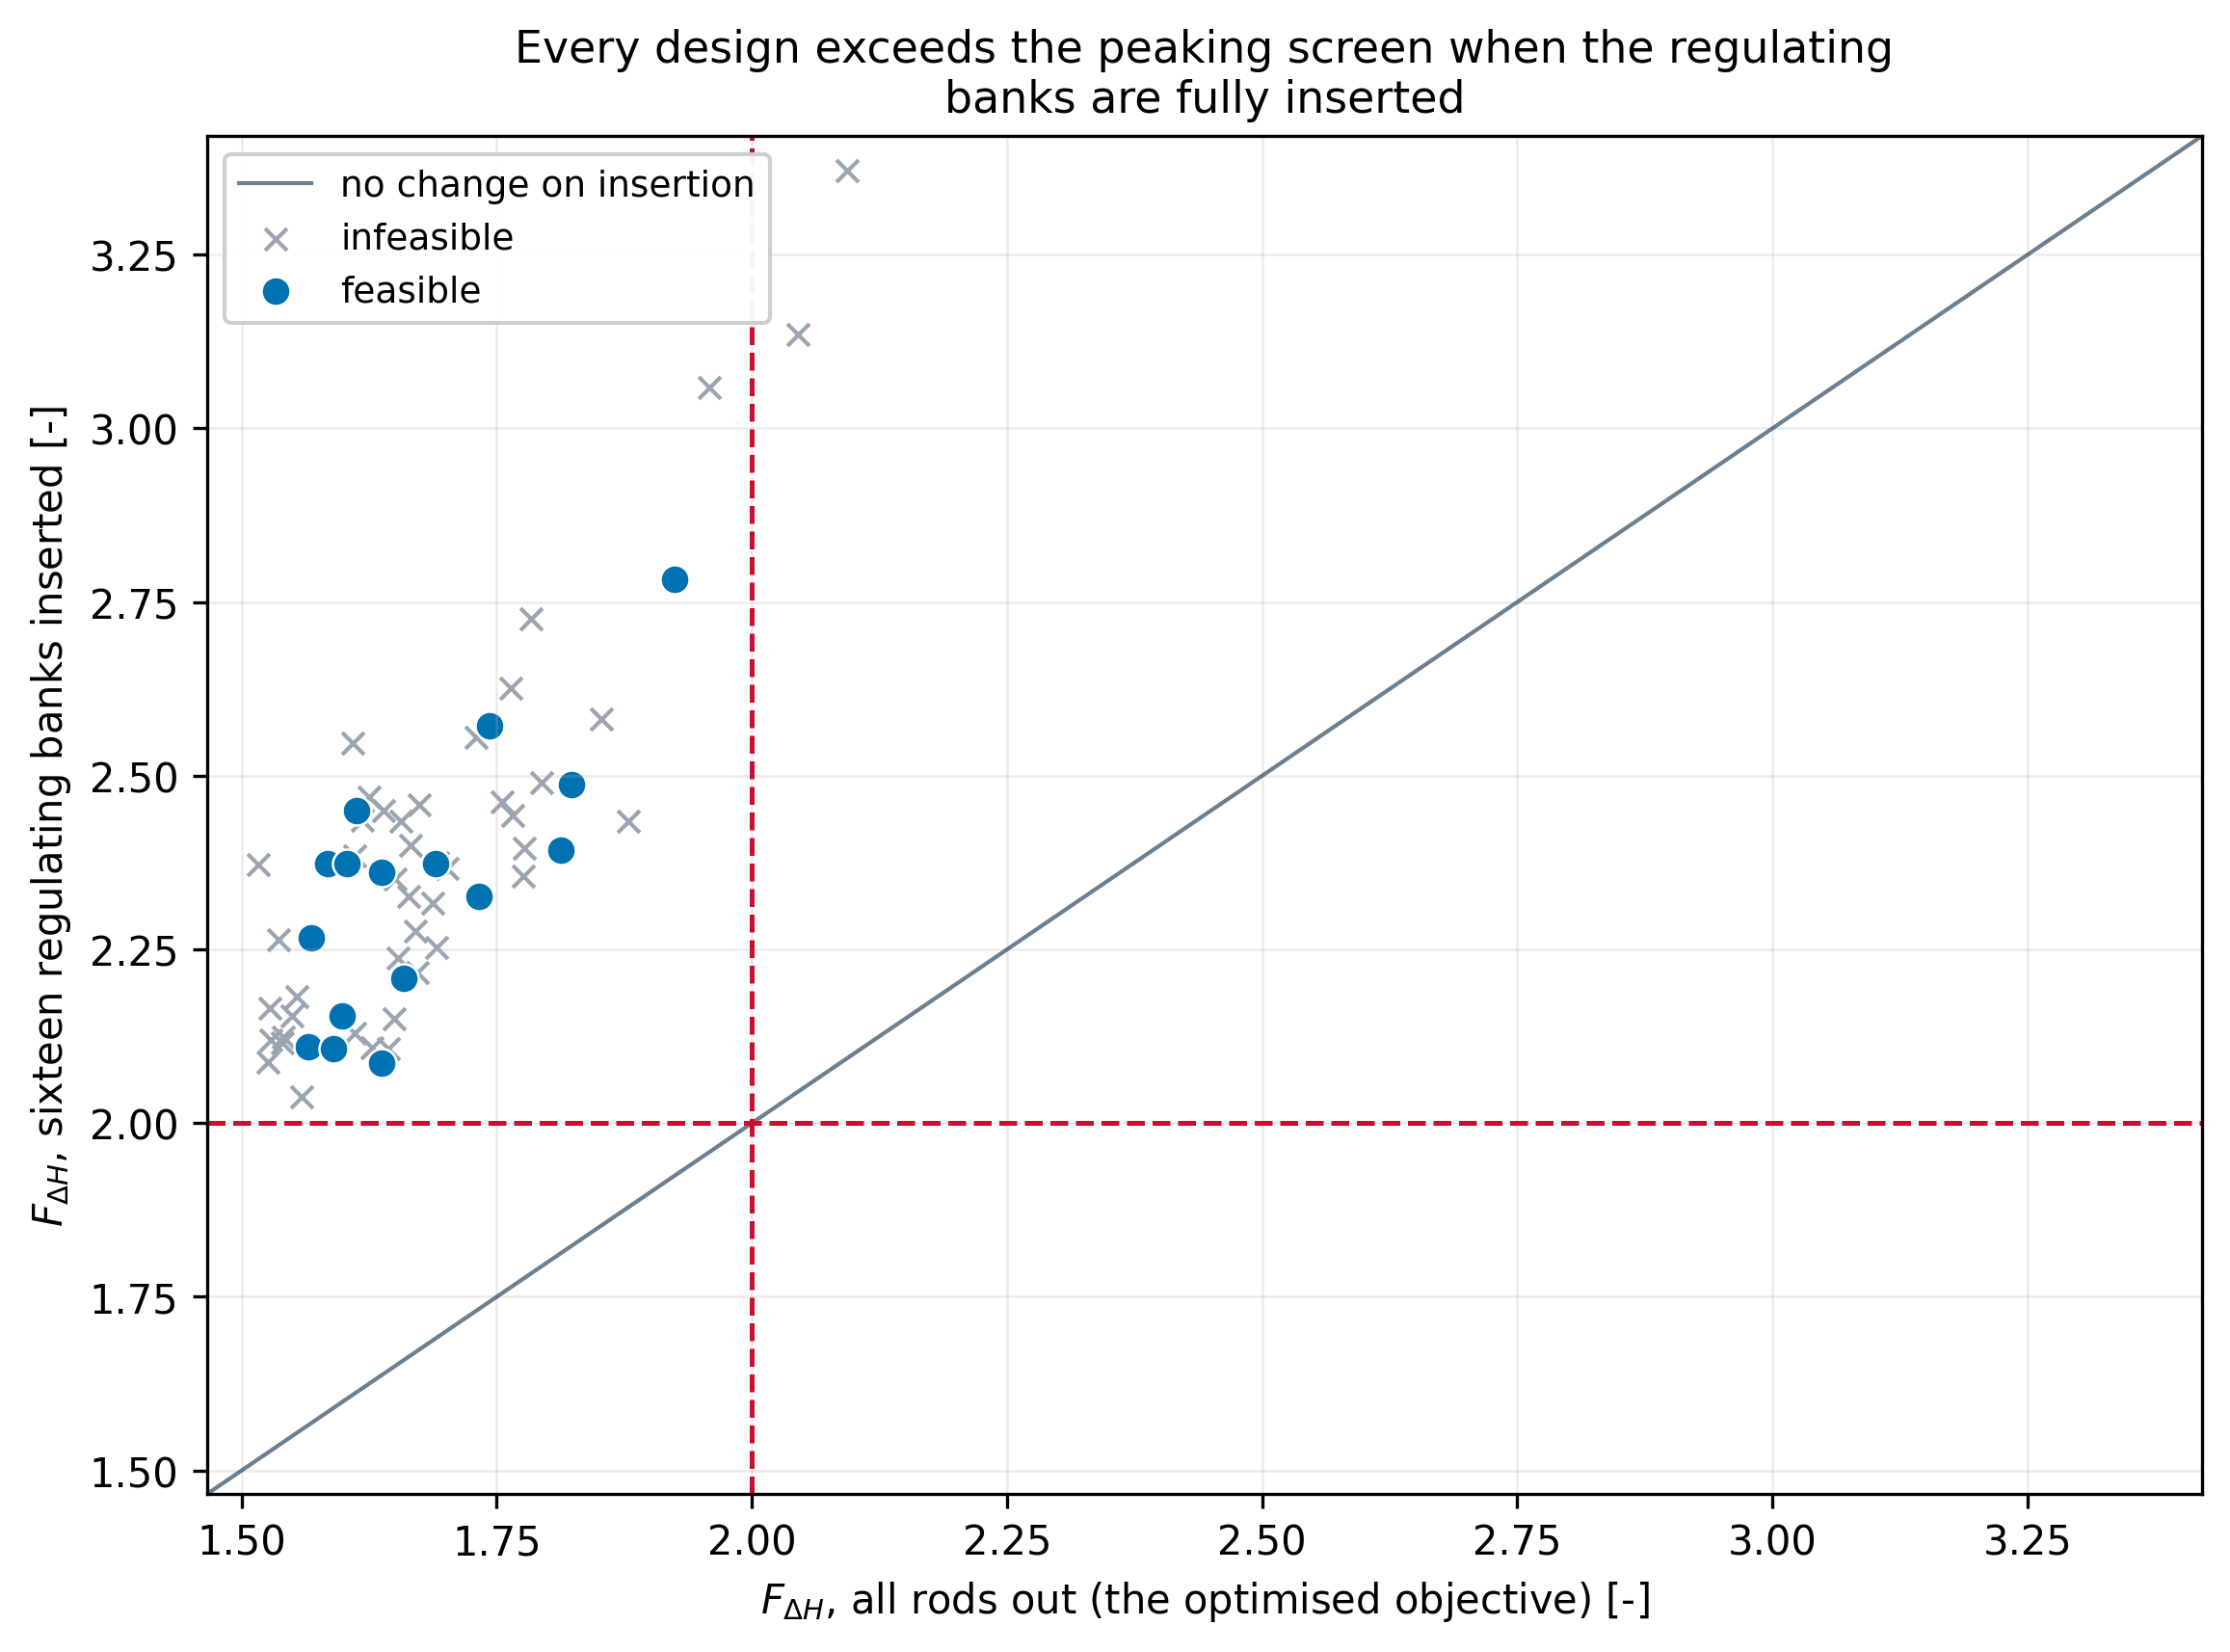
\includegraphics[width=0.85\linewidth]{images/c7_rodded_peaking}
  \caption{Radial peaking with all rods out, the optimised objective,
  against the same quantity with the sixteen regulating banks inserted.
  Every design lies above the screening bound of 2.0 in the rodded
  configuration.}
  \label{fig:c7-rodded}
\end{figure}

With the banks inserted $F_{\Delta H}$ runs from 2.038 to 3.371 with a
mean of 2.375, against 1.516 to 2.093 unrodded. The insertion penalty
ranges from 0.449 to 1.278 and is design dependent, correlating at
$-0.81$ with the outer-zone enrichment over the archive. Every one of
the 60 designs exceeds the screening bound of 2.0 in the rodded
configuration, and the three front designs sit between 2.11 and 2.16.

Two framings are required and neither should be overstated. Sixteen
banks fully inserted is the extreme of the regulating band used here as
a controllability test, not an operating configuration, so the rodded
value is an upper bound on operating peaking rather than an operating
value. Even so, the objective being minimised moves by half a unit or
more when the rods go in, and it moves by a design-dependent amount.
A design selected for low unrodded peaking is not thereby a design
with low rodded peaking. This is recorded as a limitation of the
objective set and as the motivation for the two-level reading of
Campaign 8.

%% AUTHOR: physical interpretation of the negative correlation between
%% the insertion penalty and the outer-zone enrichment.

\subsection{Depletion histories and the statistical error on the cycle length}
\label{sec:res-c7-uncertainty}

The assembly depletion solves are the only transport runs whose output
reaches the campaign log, and the log therefore holds the complete
$k_\infty(B)$ history of every design. Figure~\ref{fig:c7-histories}
reconstructs all 60 histories with the end-of-cycle crossing marked.

\begin{figure}[htbp]
  \centering
  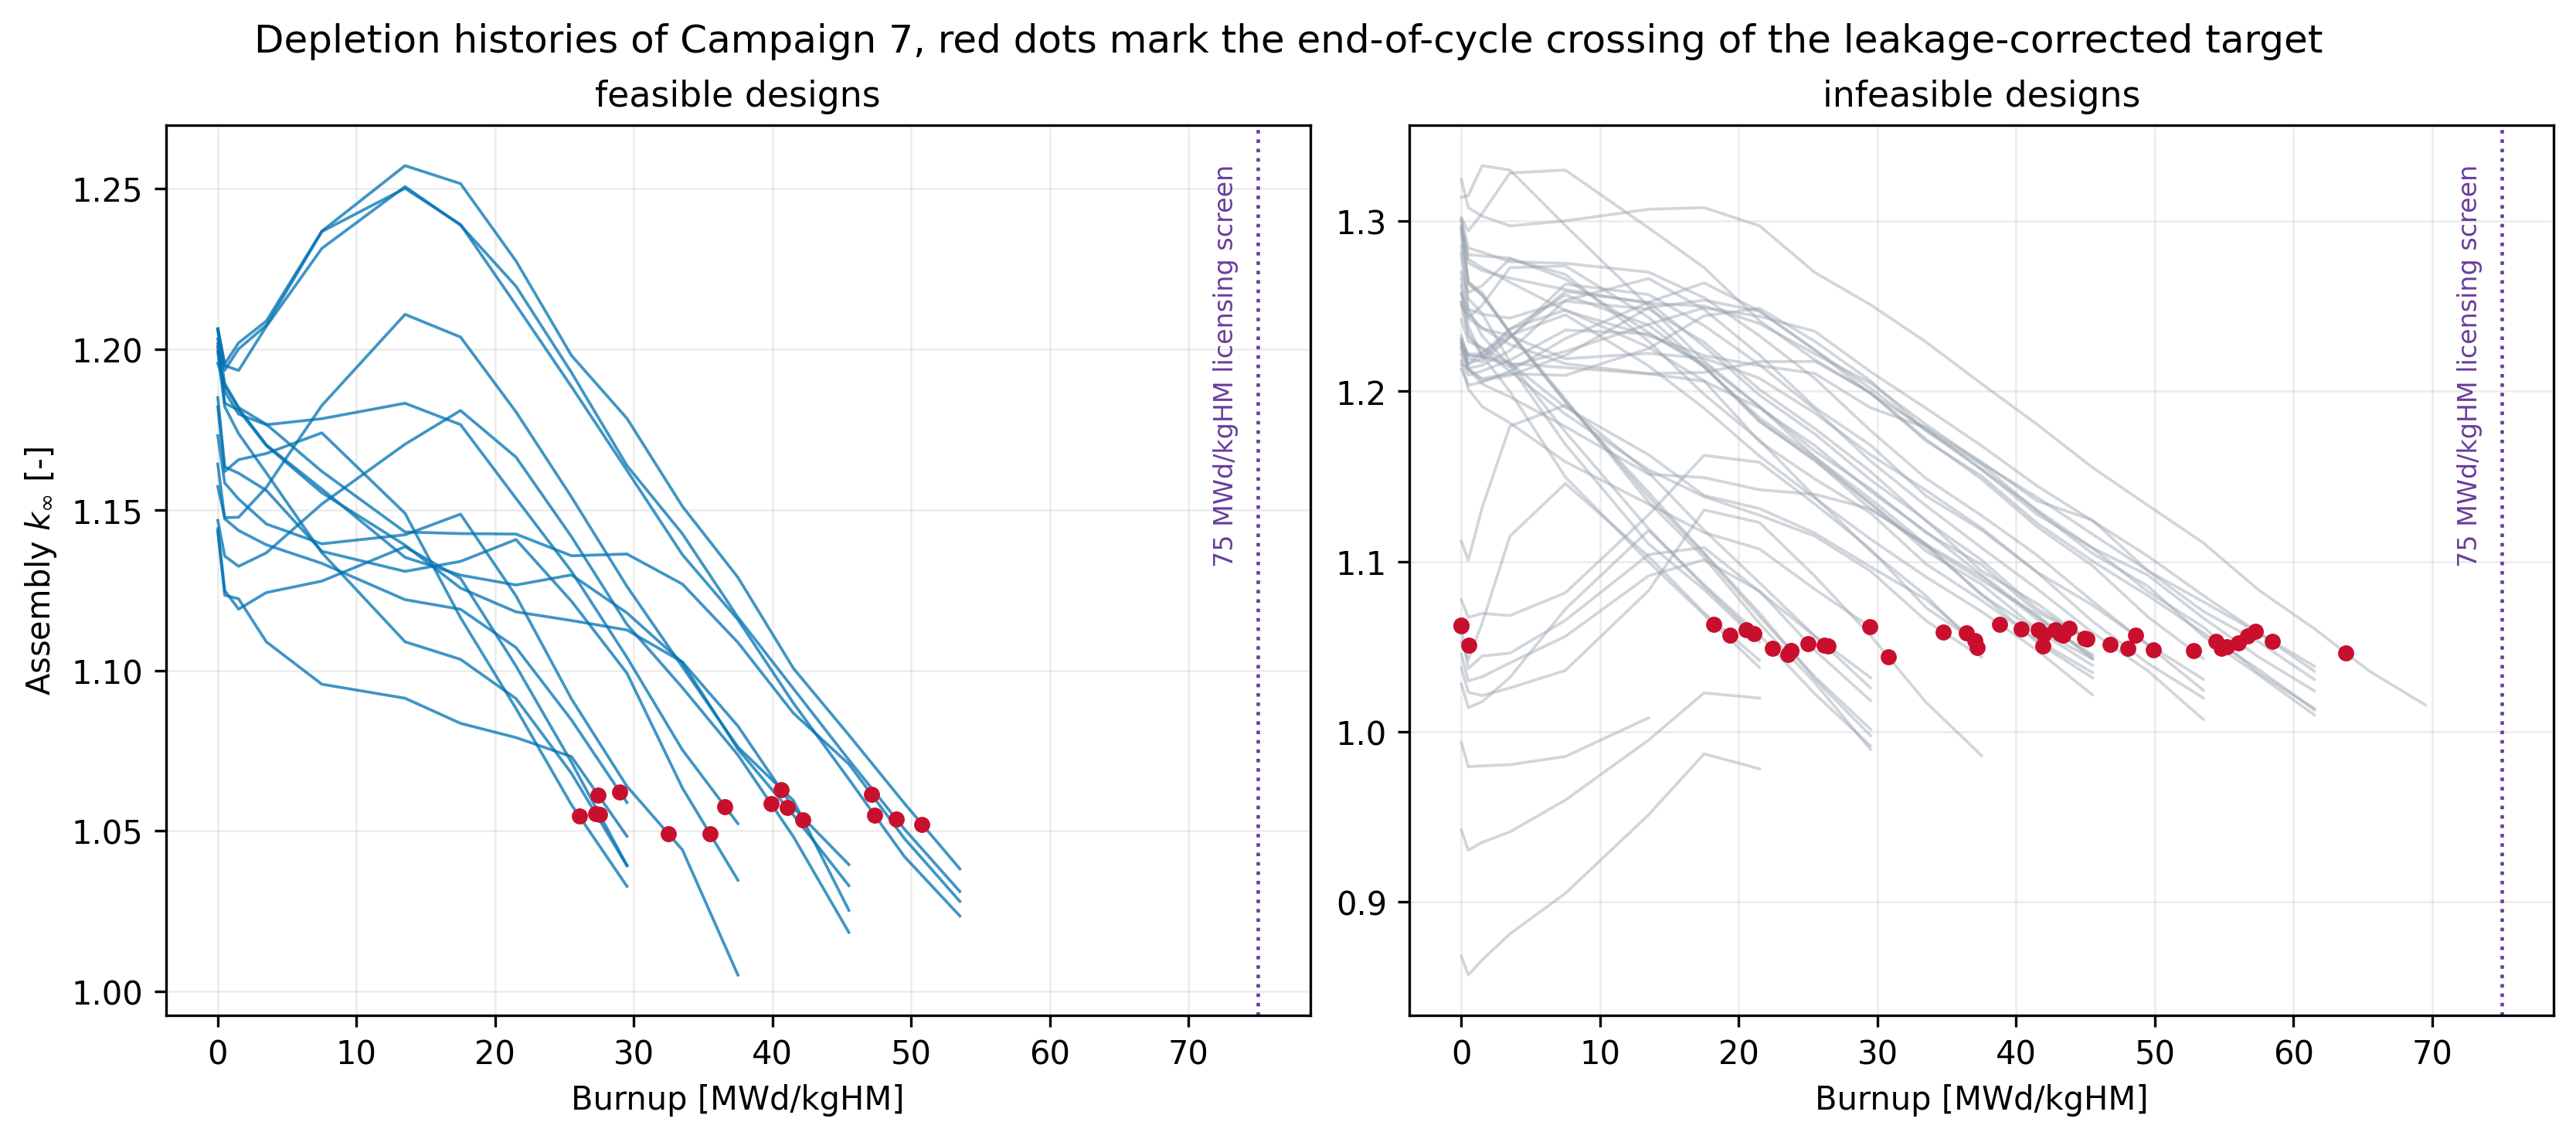
\includegraphics[width=\linewidth]{images/c7_kinf_histories}
  \caption{Assembly infinite multiplication factor against burnup for
  every Campaign 7 design, feasible designs on the left. Red markers
  are the end-of-cycle crossings of the leakage-corrected target. The
  gadolinium burnout maximum is visible between 13 and
  \SI{17}{MWd/kgHM}, and no design approaches the \SI{75}{MWd/kgHM}
  screen.}
  \label{fig:c7-histories}
\end{figure}

The reconstruction was validated against the archive. Taking the last
descending crossing of the target reproduces the stored end-of-cycle
burnup of all 57 crossing designs to within \SI{0.0011}{MWd/kgHM}. The
last crossing is the correct rule because the gadolinium burnout makes
the early history non-monotonic. The three designs without a crossing
are the two subcritical cores at zero cycle length and one design
ending at 55 EFPD.

Three facts follow from the figure. The gadolinium hump raises
$k_\infty$ by up to 0.06 before the decline. The highest end-of-cycle
burnup in the campaign is \SI{63.8}{MWd/kgHM}, so the
\SI{75}{MWd/kgHM} discharge screen of Section~\ref{sec:meth-atf} is
inactive and no design is censored, unlike Campaign 6. And the local
slope at end of cycle is steep, which governs the statistical error on
the cycle length.

The Monte Carlo error on the cycle length is obtained by propagating
the uncertainties of the two transport states that bracket the
crossing.

\begin{equation}
\sigma_B^2 = \left(\frac{\Delta B\,(k_\mathrm{t} - k_{j+1})}{(k_j - k_{j+1})^2}\right)^2 \sigma_{k_j}^2
+ \left(\frac{\Delta B\,(k_j - k_\mathrm{t})}{(k_j - k_{j+1})^2}\right)^2 \sigma_{k_{j+1}}^2
\label{eq:sigma-beoc}
\end{equation}

\noindent where the symbols have the following meaning.

\begin{itemize}
  \item $\sigma_B$ is the statistical uncertainty of the end-of-cycle
        burnup, in MWd/kgHM.

  \item $\Delta B$ is the burnup step between the two bracketing
        states, in MWd/kgHM.

  \item $k_j$ and $k_{j+1}$ are the infinite multiplication factors at
        the states before and after the crossing, dimensionless.

  \item $k_\mathrm{t}$ is the leakage-corrected target, dimensionless,
        treated as exact.

  \item $\sigma_{k_j}$ and $\sigma_{k_{j+1}}$ are the reported Monte
        Carlo standard deviations of the two states, dimensionless.
\end{itemize}

The cycle length follows from the specific power.

\begin{equation}
\sigma_\mathrm{EFPD} = \frac{1000\,\sigma_B}{P_\mathrm{sp}}
\label{eq:sigma-efpd}
\end{equation}

\noindent where the symbols have the following meaning.

\begin{itemize}
  \item $\sigma_\mathrm{EFPD}$ is the statistical uncertainty of the
        cycle length, in effective full power days.

  \item $P_\mathrm{sp}$ is the specific power of the core,
        \SI{9.98}{W/gHM}.
\end{itemize}

\begin{figure}[htbp]
  \centering
  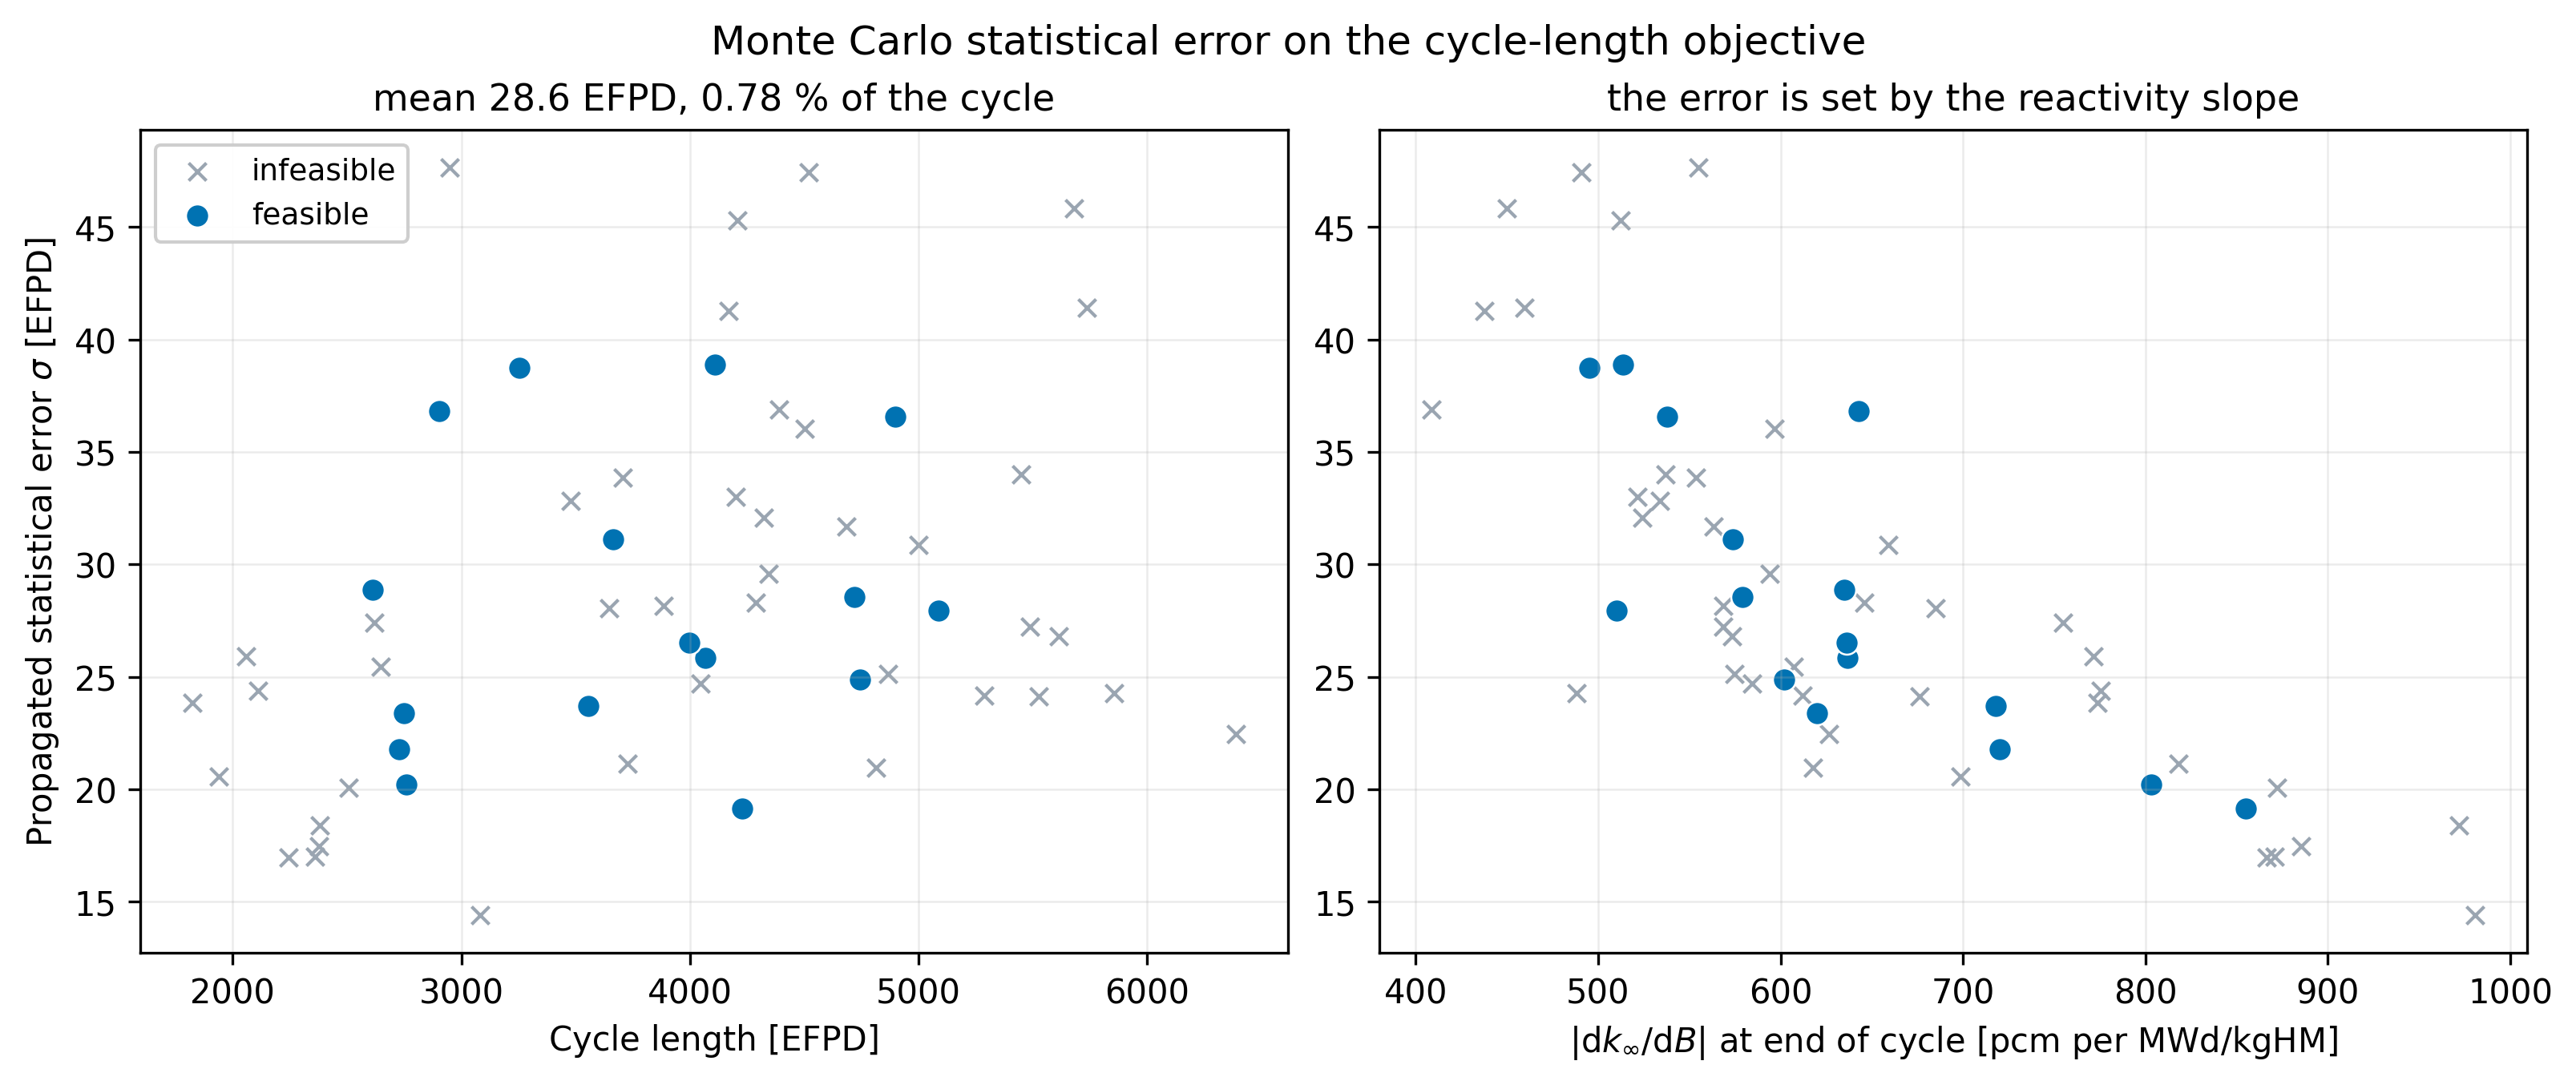
\includegraphics[width=\linewidth]{images/c7_cycle_uncertainty}
  \caption{Propagated Monte Carlo error on the cycle length against the
  cycle length and against the reactivity slope at end of cycle. The
  error is set by the slope, not by the length of the cycle.}
  \label{fig:c7-uncertainty}
\end{figure}

Table~\ref{tab:c7-uncertainty} summarises the result and
Figure~\ref{fig:c7-uncertainty} shows it. The slope at end of cycle
lies between 409 and \SI{981}{pcm} per MWd/kgHM with a median of 607.
The resulting error has a mean of 28.6 EFPD, \SI{0.78}{\%} of the
cycle, and a worst case of 47.7 EFPD, \SI{1.62}{\%}. On the six front
designs it is 25 to 37 EFPD. The smallest gap between adjacent front
designs is 154 EFPD, about five standard deviations, so the ordering of
the front in cycle length is statistically resolved.

\begin{table}[htbp]
  \centering
  \caption{Statistical error on the cycle length over the 57 designs
  with a resolved end-of-cycle crossing.}
  \label{tab:c7-uncertainty}
  \begin{tabular}{lccc}
    \toprule
    Quantity & Minimum & Median & Maximum \\
    \midrule
    Slope at end of cycle [pcm per MWd/kgHM] & 409 & 607 & 981 \\
    Bracketing sigma on $k_\infty$ [pcm]     & 178 & 218 & 274 \\
    $\sigma_\mathrm{EFPD}$ [d]               & 14.4 & 27.2 & 47.7 \\
    $\sigma_\mathrm{EFPD}$ as a fraction of the cycle [\%] & 0.35 & 0.74 & 1.62 \\
    \bottomrule
  \end{tabular}
\end{table}

The peaking axis is the opposite case. The front designs are separated
by 0.003 to 0.036 in $F_{\Delta H}$, the entropy study of
Section~\ref{sec:res-c6} bounded the systematic shift at $\pm 0.02$,
and no statistical error on the core peaking tally has been measured.
The ordering of the front in peaking is therefore not resolved, and
designs 59, 57 and 55 at 1.525, 1.528 and 1.529 must be treated as
indistinguishable until the tally errors are read from the statepoints.

\openpoint{Measure $\sigma(F_{\Delta H})$ from the per-bin relative
errors of the core mesh tally on the six front designs, or by seed
replicates, before any ordering claim on the peaking axis is made.}

\subsection{Cost and instrumentation}
\label{sec:res-c7-cost}

The campaign cost \SI{56965}{s} of wall time, \SI{949}{s} per
evaluation, against \SI{840}{s} in Campaign 6. The difference is the
control solve. Two instrumentation defects were found while reading
the archive, and both are recorded because they affect numbers reported
elsewhere in this chapter.

\begin{enumerate}
  \item The per-evaluation cost stored in the archive excludes the
        control solve, because that solve is invoked after the three
        timers close. Over the campaign the control solves are
        \SI{11}{\%} of the true cost and \SI{12.6}{\%} of the reported
        cost. The wall-clock figure of the block log is correct and is
        the one quoted above. The evaluator is corrected from Campaign
        8 (Section~\ref{sec:meth-cost}).

  \item The per-case parser of the run log never matched a single case
        line of any campaign, because the censoring marker inserted
        after the cycle length was not anticipated by its regular
        expression. The failure was silent, and every per-case table
        the parser produced before the correction was empty. No number
        in this chapter depends on that table, since all per-design
        quantities are read from the archive.
\end{enumerate}

\subsection{Limitations and what carries forward}
\label{sec:res-c7-limits}

Four limitations bound the claims of this section.

\begin{enumerate}
  \item Four designs, 10, 32, 41 and 43, reached the active batches
        with the Shannon entropy of the fission source not yet
        converged, the worst at 105 of 60 inactive batches. None is on
        either front. Their eigenvalues and peaking values carry an
        unquantified bias, are retained in the archive statistics of
        this section with that caveat, and are excluded from any
        candidate list.

  \item Twenty-five of the 60 designs have a pitch below
        \SI{1.2242}{cm}, twice the guide-tube outer radius. Below that
        value the lattice clips the guide-tube wall at the cell
        boundary silently, replacing up to \SI{27}{\%} of the wall
        cross-section by moderator at the box minimum of
        \SI{1.150}{cm}. Designs 57 and 59, the two lowest-peaking
        designs of the control-screen front, are both in the affected
        band. The same defect reaches back to every earlier campaign
        design at pitches below \SI{1.2242}{cm}, including the
        Campaign 4 infill designs pinned at the box minimum and the
        Campaign 6 discharge-screen champion at \SI{1.150}{cm}. Fixing
        the pitch at \SI{1.26}{cm} in Campaign 8 removes the defect
        prospectively, and a caveat is added to the affected results.

  \item The statistical error on the peaking objective is not
        measured, as stated above.

  \item Every cycle length in this campaign, as in all earlier ones, is
        a two-dimensional value. The axial leakage study of
        Section~\ref{sec:meth-lax}, completed after this campaign,
        measured the axial correction at \num{1.0282} to \num{1.0298}
        on six Campaign 6 designs, about \SI{3000}{pcm} of reactivity,
        which at the end-of-cycle slopes measured here corresponds to
        roughly 450 to 500 EFPD. Campaign 7 cycle lengths are therefore
        overstated by that amount relative to a finite-height core,
        uniformly across the archive, and the ordering of the front is
        unaffected. Campaign 8 carries the correction inside the
        end-of-cycle target from the start.
\end{enumerate}

What carries forward is the constraint architecture. The measured
control screen replaces the derived ceiling as the reactivity
constraint that does the work, a second reading with only the first two
banks inserted is added and recorded, the axial factor enters the
target, the acquisition settings of Campaign 6 are restored explicitly,
and the pitch is fixed at the value that both closes the geometric
defect and matches the reference fuel design. Section~\ref{sec:res-c8}
states the campaign built on those decisions.
 at that point.
%
%  Figures: copy the eight PDF files of c7_analysis_60/ into images/.
%    c7_pareto_60, c7_ctrl_screen, c7_rod_worth, c7_rodded_peaking,
%    c7_kinf_histories, c7_cycle_uncertainty, c7_infill_diversity,
%    c7_vars_influence
%
%  Labels defined here: sec:res-c7, sec:res-c7-basis, sec:res-c7-blocks,
%  sec:res-c7-screens, sec:res-c7-worth, sec:res-c7-rodded,
%  sec:res-c7-uncertainty, sec:res-c7-cost, sec:res-c7-limits,
%  tab:c7-blocks, tab:c7-front, tab:c7-nesting, tab:c7-uncertainty,
%  fig:c7-diversity, fig:c7-screens, fig:c7-pareto, fig:c7-worth,
%  fig:c7-influence, fig:c7-rodded, fig:c7-histories, fig:c7-uncertainty,
%  eq:g-ctrl, eq:k-implied, eq:bank-worth, eq:sigma-beoc, eq:sigma-efpd
%
%  Labels used from elsewhere: sec:meth-ctrl, sec:meth-ktarget,
%  sec:meth-acq, sec:res-c6, sec:res-c6-blocks, tab:fidelity,
%  sec:meth-lax, sec:res-c8, sec:meth-cost. Define sec:meth-ctrl,
%  sec:meth-lax and sec:meth-cost with methodology_c78_additions.tex.
%
%  Style: short paragraphs, no semicolons, no em dashes, every displayed
%  formula followed by a term list with units, enumerations as lists.
% =====================================================================

\section{Campaign 7: the controllability screen}
\label{sec:res-c7}

Campaign 6 closed with a front whose long-cycle end rode the
reactivity ceiling, and with the observation that the ceiling of 1.35
proxied controllable excess reactivity without a rod model. Campaign 7
replaces the proxy by a measurement. Every evaluation now solves the
beginning-of-life core a second time with the sixteen regulating-bank
control rod assemblies inserted, and the resulting eigenvalue enters the
constraint set directly. The campaign ran 60 evaluations on the AWS
instance in \SI{15.82}{h}, and every one of them completed without
error.

\subsection{The one change and its two consequences}
\label{sec:res-c7-basis}

The constraint added is the controllability screen of
Section~\ref{sec:meth-ctrl}.

\begin{equation}
g_\mathrm{ctrl}(\mathbf{x}) = k_\mathrm{ARI}(\mathbf{x}) - (1 - \Delta\rho_\mathrm{op}) \le 0
\label{eq:g-ctrl}
\end{equation}

\noindent where the symbols have the following meaning.

\begin{itemize}
  \item $k_\mathrm{ARI}$ is the effective multiplication factor of the
        32-assembly core at beginning of life with all sixteen
        regulating-bank assemblies inserted and the shutdown banks
        withdrawn, dimensionless.

  \item $\Delta\rho_\mathrm{op}$ is the operating subcriticality margin
        demanded of the regulating banks, \num{0.01} in units of $k$,
        that is \SI{1000}{pcm}.

  \item $\mathbf{x}$ is the design vector.
\end{itemize}

Two settings changed with it. The reactivity ceiling was lowered from
1.35 to 1.126, a value derived before the campaign from the smallest
regulating-bank worth measured on eight Campaign 6 designs, and the
enrichment cap was lowered to \SI{12}{wt\%} on the as-built peripheral
ring, giving a search box of 3.0 to \SI{10.43}{wt\%}. Both were
intended as consequences of the controllability requirement rather than
as independent changes, and the campaign tests whether they were
consistent with the measurement they were meant to anticipate.

\subsection{Design of experiments and the three infill blocks}
\label{sec:res-c7-blocks}

The campaign ran a design of experiments of 42 followed by three infill
blocks of six. Table~\ref{tab:c7-blocks} records the outcome of each
block and Figure~\ref{fig:c7-diversity} its diversity, measured as the
spread of each design variable within the block as a fraction of the
range spanned by the whole archive.

\begin{table}[htbp]
  \centering
  \caption{Campaign 7 blocks. The hypervolume is the frozen-reference
  value written at each block boundary. Spread is the within-block
  range of each variable as a fraction of the archive range, listed
  for the four non-geometric variables.}
  \label{tab:c7-blocks}
  \begin{tabular}{lccll}
    \toprule
    Block & Designs & Feasible & Hypervolume & Spread in $e_\mathrm{in}$, $e_\mathrm{out}$, $w_\mathrm{Gd}$, $n_\mathrm{Gd}$ \\
    \midrule
    DOE      & 42 & 13 & 773.7 & 0.98 to 1.00 \\
    Infill 1 &  6 &  0 & 773.7 & 0.000 to 0.002 \\
    Infill 2 &  6 &  3 & 996.5 & 0.07 to 0.29 \\
    Infill 3 &  6 &  0 & 996.5 & 0.015 to 0.13 \\
    \bottomrule
  \end{tabular}
\end{table}

\begin{figure}[htbp]
  \centering
  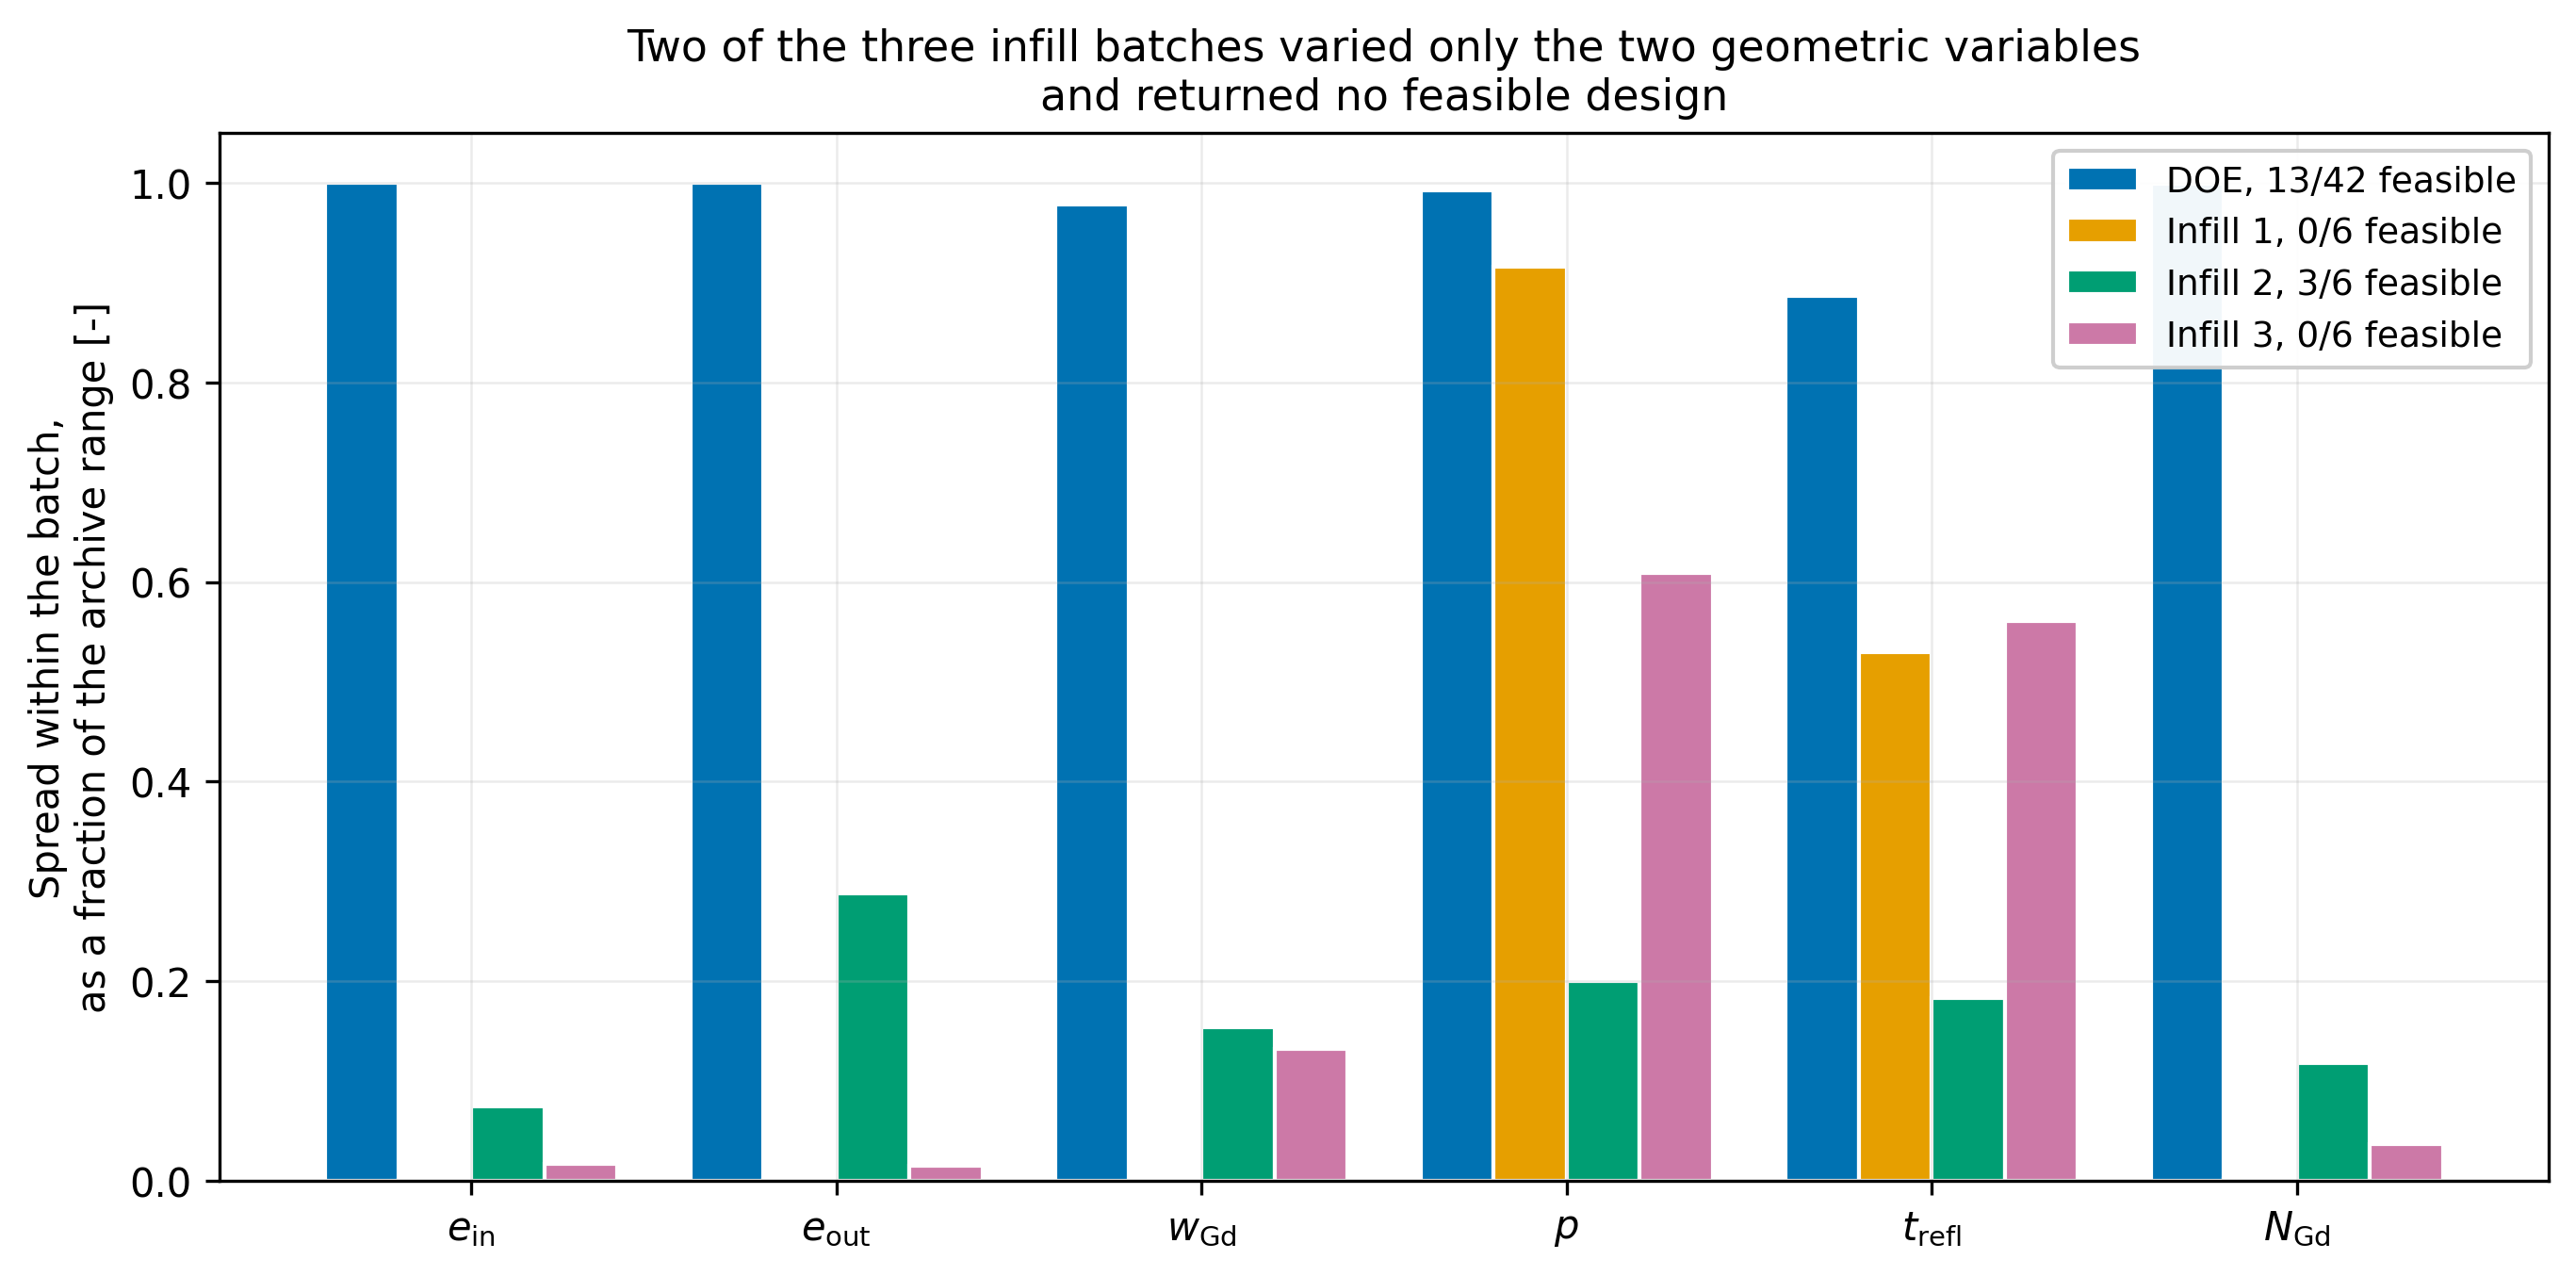
\includegraphics[width=\linewidth]{images/c7_infill_diversity}
  \caption{Within-block spread of each design variable, as a fraction
  of the archive range. Infill blocks 1 and 3 vary only the pitch and
  the reflector thickness, and neither returned a feasible design.}
  \label{fig:c7-diversity}
\end{figure}

Two of the three infill blocks collapsed. In block 1 the six designs
share one enrichment pair, \num{5.09} and \SI{4.04}{wt\%}, exactly zero
gadolinia and 24 poisoned pins, and differ only in pitch and reflector
thickness. In block 3 the same pattern recurs at \num{8.13} and
\SI{7.33}{wt\%} with 32 pins. All twelve designs of the two blocks
failed the reactivity ceiling.

The cause is a configuration regression, not a new defect. The
acquisition ran with a minimum separation of 0.05 and a feasibility
margin of 1.0 standard deviation, the default values of the launcher,
where Campaign 6 had established 0.14 and 1.5 in
Section~\ref{sec:res-c6-blocks}. The two collapsed blocks satisfied the
separation rule as coded, with pairwise separations of 0.059 to 0.089,
because the rule averages over all six variables and two of them
supplied the whole distance. A per-variable minimum spread would have
rejected both batches.

The consequence for the convergence record is that the flat
hypervolume of block 3 is not a stopping signal. Under the Campaign 6
rule a zero gain counts toward stopping only when the acquisition is
functioning, and block 3 demonstrably was not. The campaign therefore
ends with an unconverged front, and its value lies in the constraint
measurements rather than in the front itself.

\subsection{Feasibility and the nesting of the two screens}
\label{sec:res-c7-screens}

Of the 60 designs, 16 are feasible against all six constraints, a
fraction of \SI{26.7}{\%} against \SI{67}{\%} in the Campaign 6 design
of experiments. Table~\ref{tab:c7-nesting} gives the constraint census.
No design fails the enrichment or the geometric constraint, two fail
the peaking limit, nine fall below the reactivity floor, 34 exceed the
ceiling and 20 fail the controllability screen.

\begin{table}[htbp]
  \centering
  \caption{Constraint census of Campaign 7 and the joint activity of
  the two reactivity screens. Every design that fails the
  controllability screen also fails the derived ceiling, and fourteen
  designs fail the ceiling while passing the controllability screen.}
  \label{tab:c7-nesting}
  \begin{tabular}{lc}
    \toprule
    Outcome & Designs \\
    \midrule
    Fail $g_{k\max}$ at 1.126                      & 34 \\
    Fail $g_\mathrm{ctrl}$                         & 20 \\
    Fail $g_\mathrm{ctrl}$ and pass $g_{k\max}$    &  0 \\
    Fail $g_{k\max}$ and pass $g_\mathrm{ctrl}$    & 14 \\
    Pass every constraint except $g_{k\max}$       & 14 \\
    Feasible on all six                            & 16 \\
    \bottomrule
  \end{tabular}
\end{table}

\begin{figure}[htbp]
  \centering
  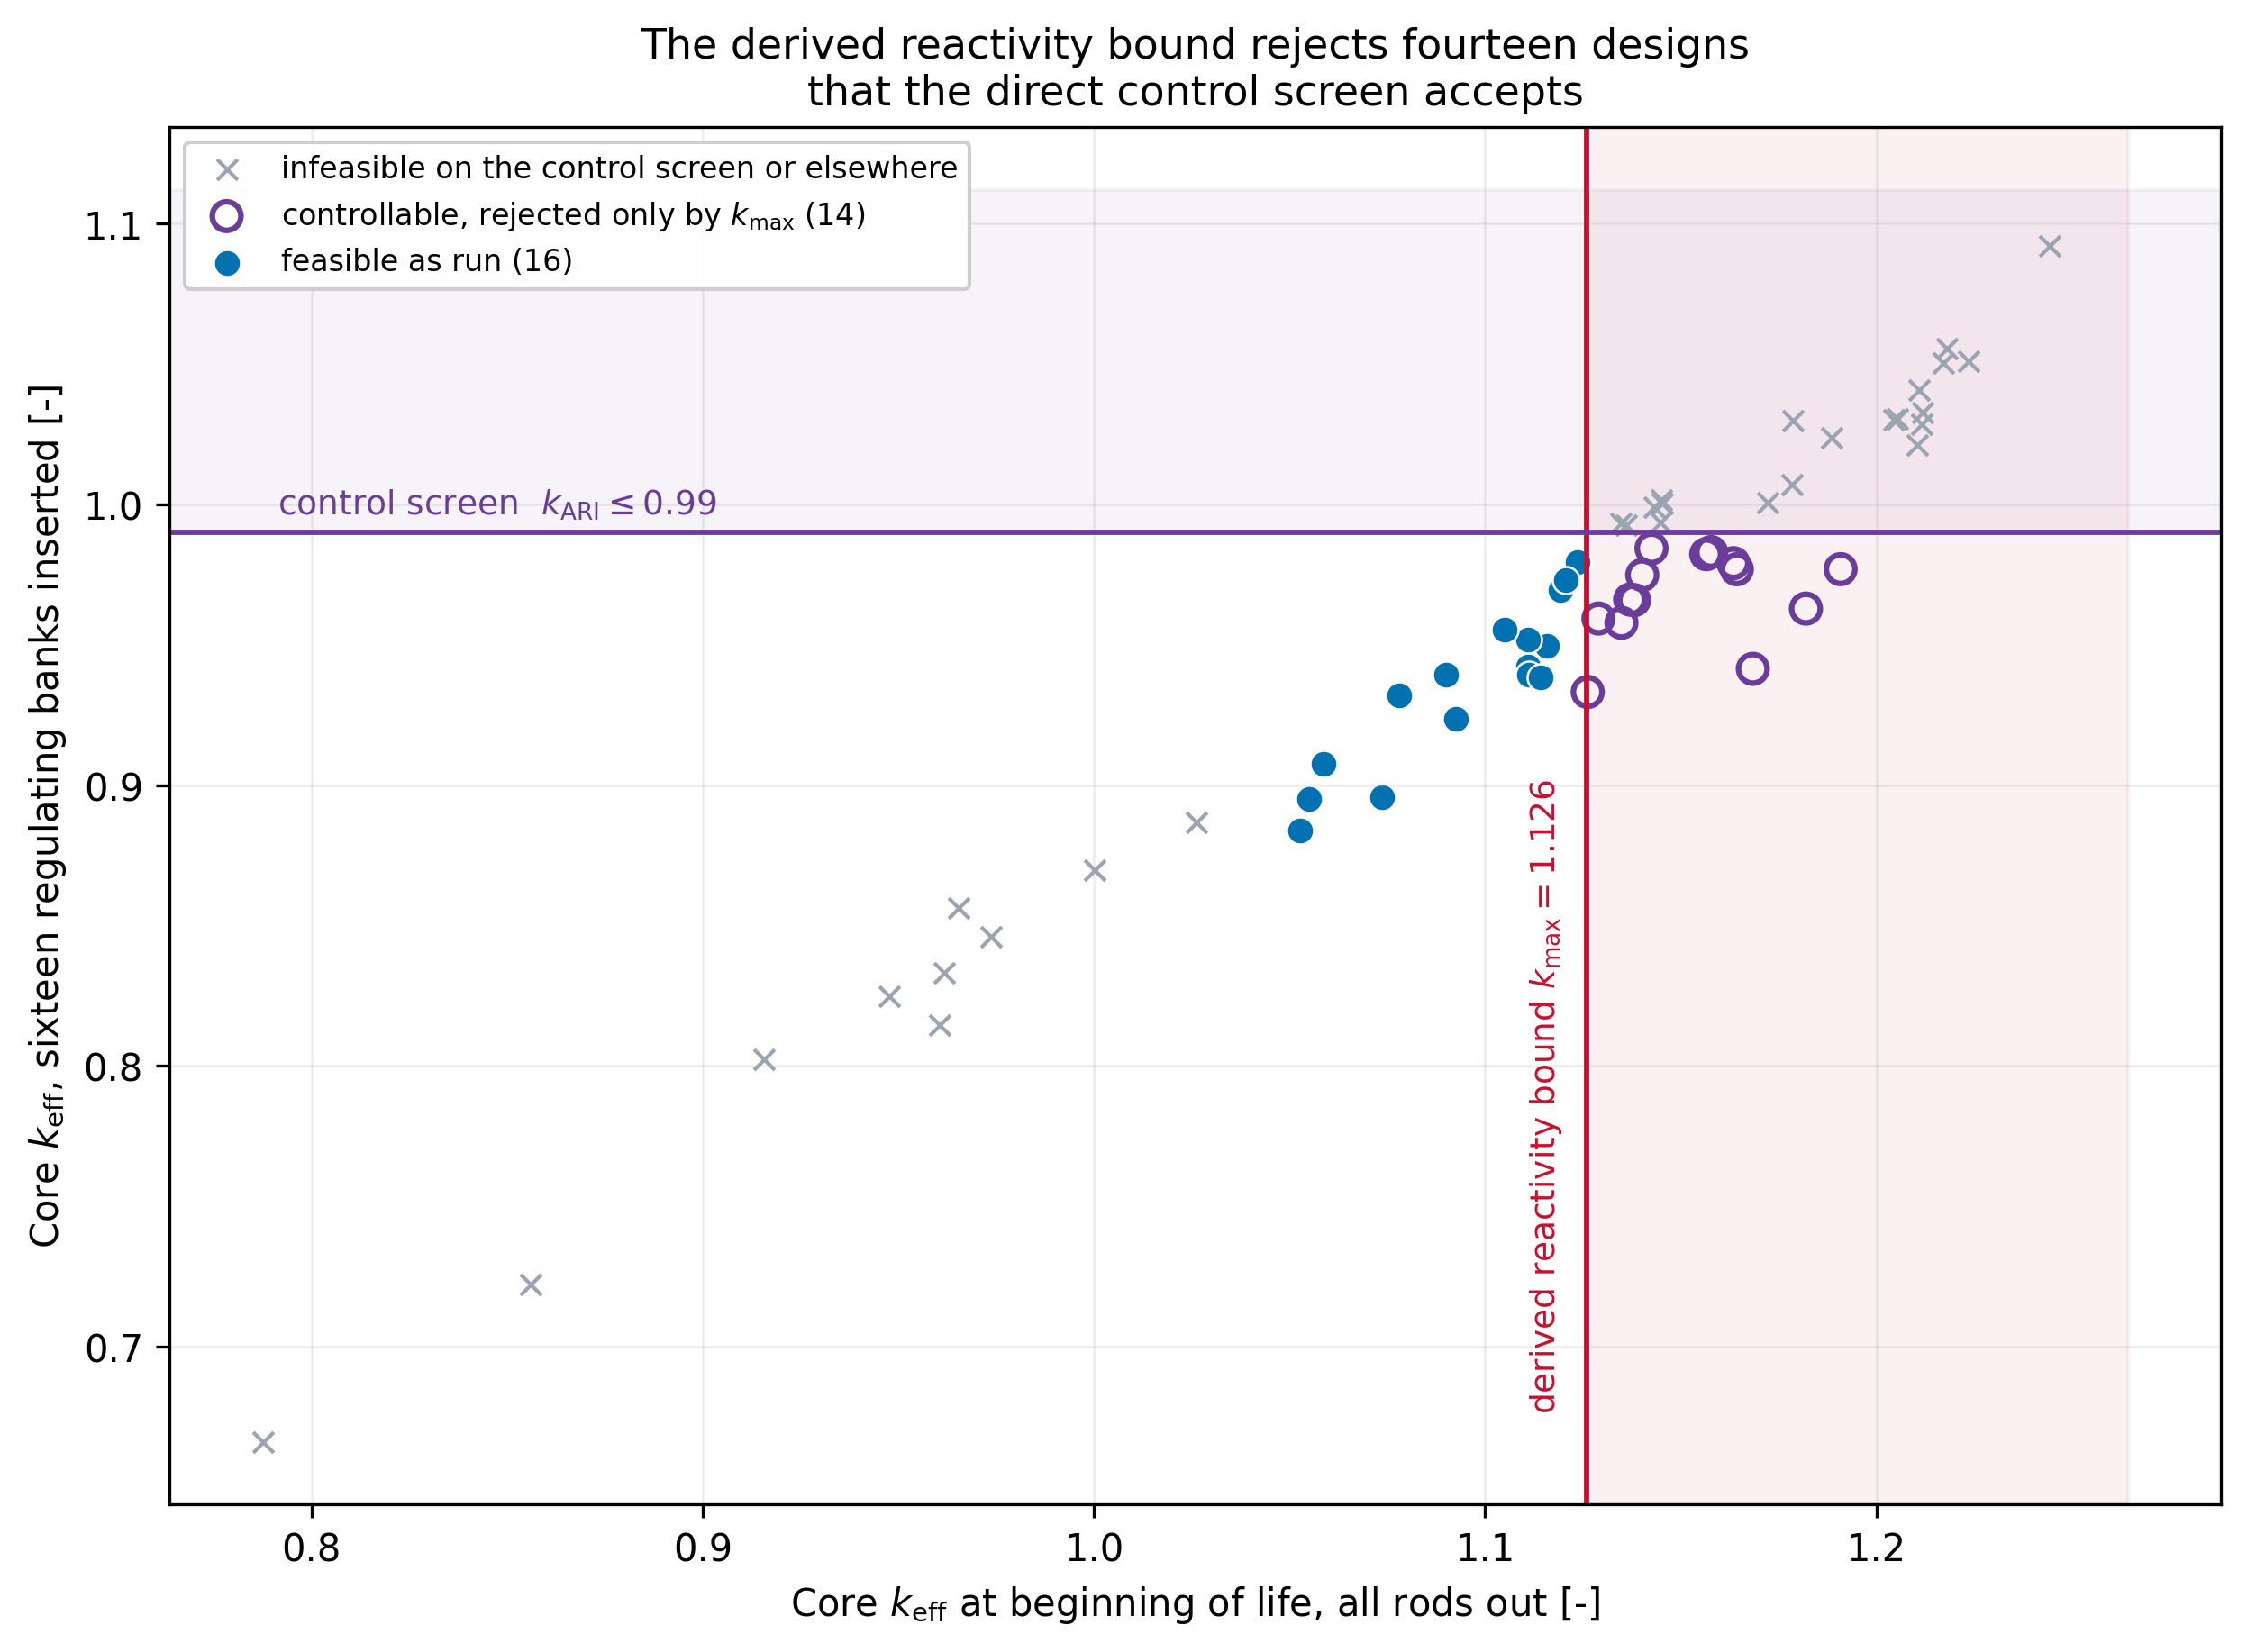
\includegraphics[width=0.9\linewidth]{images/c7_ctrl_screen}
  \caption{The two reactivity screens of Campaign 7 in the plane of
  the unrodded and the all-regulating-banks-in core eigenvalues. The
  derived ceiling at 1.126 rejects fourteen designs, marked by open
  circles, that the directly measured control screen accepts.}
  \label{fig:c7-screens}
\end{figure}

The two screens are nested. Not one design in the archive fails the
control screen without also failing the derived ceiling, and fourteen
designs fail the ceiling while their own measured bank worth shows them
controllable at the stated margin. Figure~\ref{fig:c7-screens} shows
the nesting directly. The ceiling of 1.126 therefore did no work that
the measurement did not do, and it discarded fourteen evaluations that
the measurement would have kept.

The derivation explains why. The eight Campaign 6 designs from which
1.126 was obtained had worths between \num{12174} and
\SI{12718}{pcm}, a spread of four per cent. The 60 designs of this
campaign span \num{10936} to \SI{22699}{pcm}, a factor of two. Eight
near-identical designs under-sampled the variability by an order of
magnitude, and the resulting bound is at once too tight where it
matters and not conservative in general. Restricted to the 22 designs
with an unrodded eigenvalue between 1.09 and 1.17, the smallest
measured worth of \SI{14126}{pcm} implies a ceiling of 1.151, while the
smallest worth in the whole archive implies 1.110.

The front reflects the same fact. As run, the feasible non-dominated set
holds three designs, all from infill block 2. With the derived ceiling
removed and the measured control screen retained, the feasible set grows
from 16 to 30 designs, the front doubles to six, the peaking floor moves
from 1.565 to 1.525, and the hypervolume against the frozen reference
rises from 996.5 to 1054.1, a gain of \SI{5.8}{\%}. Three of the six
designs come from infill block 3, the block that under the ceiling
contributed nothing. Table~\ref{tab:c7-front} lists both fronts and
Figure~\ref{fig:c7-pareto} places them in the objective plane.

\begin{table}[htbp]
  \centering
  \small
  \caption{The Campaign 7 front under the two screening rules. Designs
  48, 53 and 49 form the front as run. All six form the front when the
  measured control screen alone governs reactivity. Bank worth is the
  difference between the unrodded and the all-banks-in eigenvalues.}
  \label{tab:c7-front}
  \begin{tabular}{ccccccccccc}
    \toprule
    Design & EFPD & $F_{\Delta H}$ & $e_\mathrm{in}$ & $e_\mathrm{out}$ & $w_\mathrm{Gd}$ & $p$ & $t_\mathrm{refl}$ & $n_\mathrm{Gd}$ & $k_\mathrm{eff}^\mathrm{core}$ & worth \\
           & [d] & [-] & [wt\%] & [wt\%] & [wt\%] & [cm] & [cm] & [-] & [-] & [pcm] \\
    \midrule
    59 & 3886 & 1.525 & 8.13 & 7.33 & 1.10 & 1.150 & 19.49 & 32 & 1.135 & 17699 \\
    57 & 4045 & 1.528 & 8.13 & 7.33 & 1.21 & 1.176 & 17.87 & 32 & 1.137 & 17094 \\
    55 & 4502 & 1.529 & 8.14 & 7.34 & 1.10 & 1.238 & 14.09 & 32 & 1.143 & 15815 \\
    48 & 4745 & 1.565 & 8.71 & 7.80 & 1.93 & 1.237 & 14.06 & 40 & 1.119 & 14970 \\
    53 & 4899 & 1.590 & 8.97 & 7.88 & 1.96 & 1.249 & 13.21 & 40 & 1.121 & 14734 \\
    49 & 5087 & 1.598 & 9.19 & 8.30 & 2.13 & 1.267 & 12.29 & 40 & 1.124 & 14416 \\
    \bottomrule
  \end{tabular}
\end{table}

\begin{figure}[htbp]
  \centering
  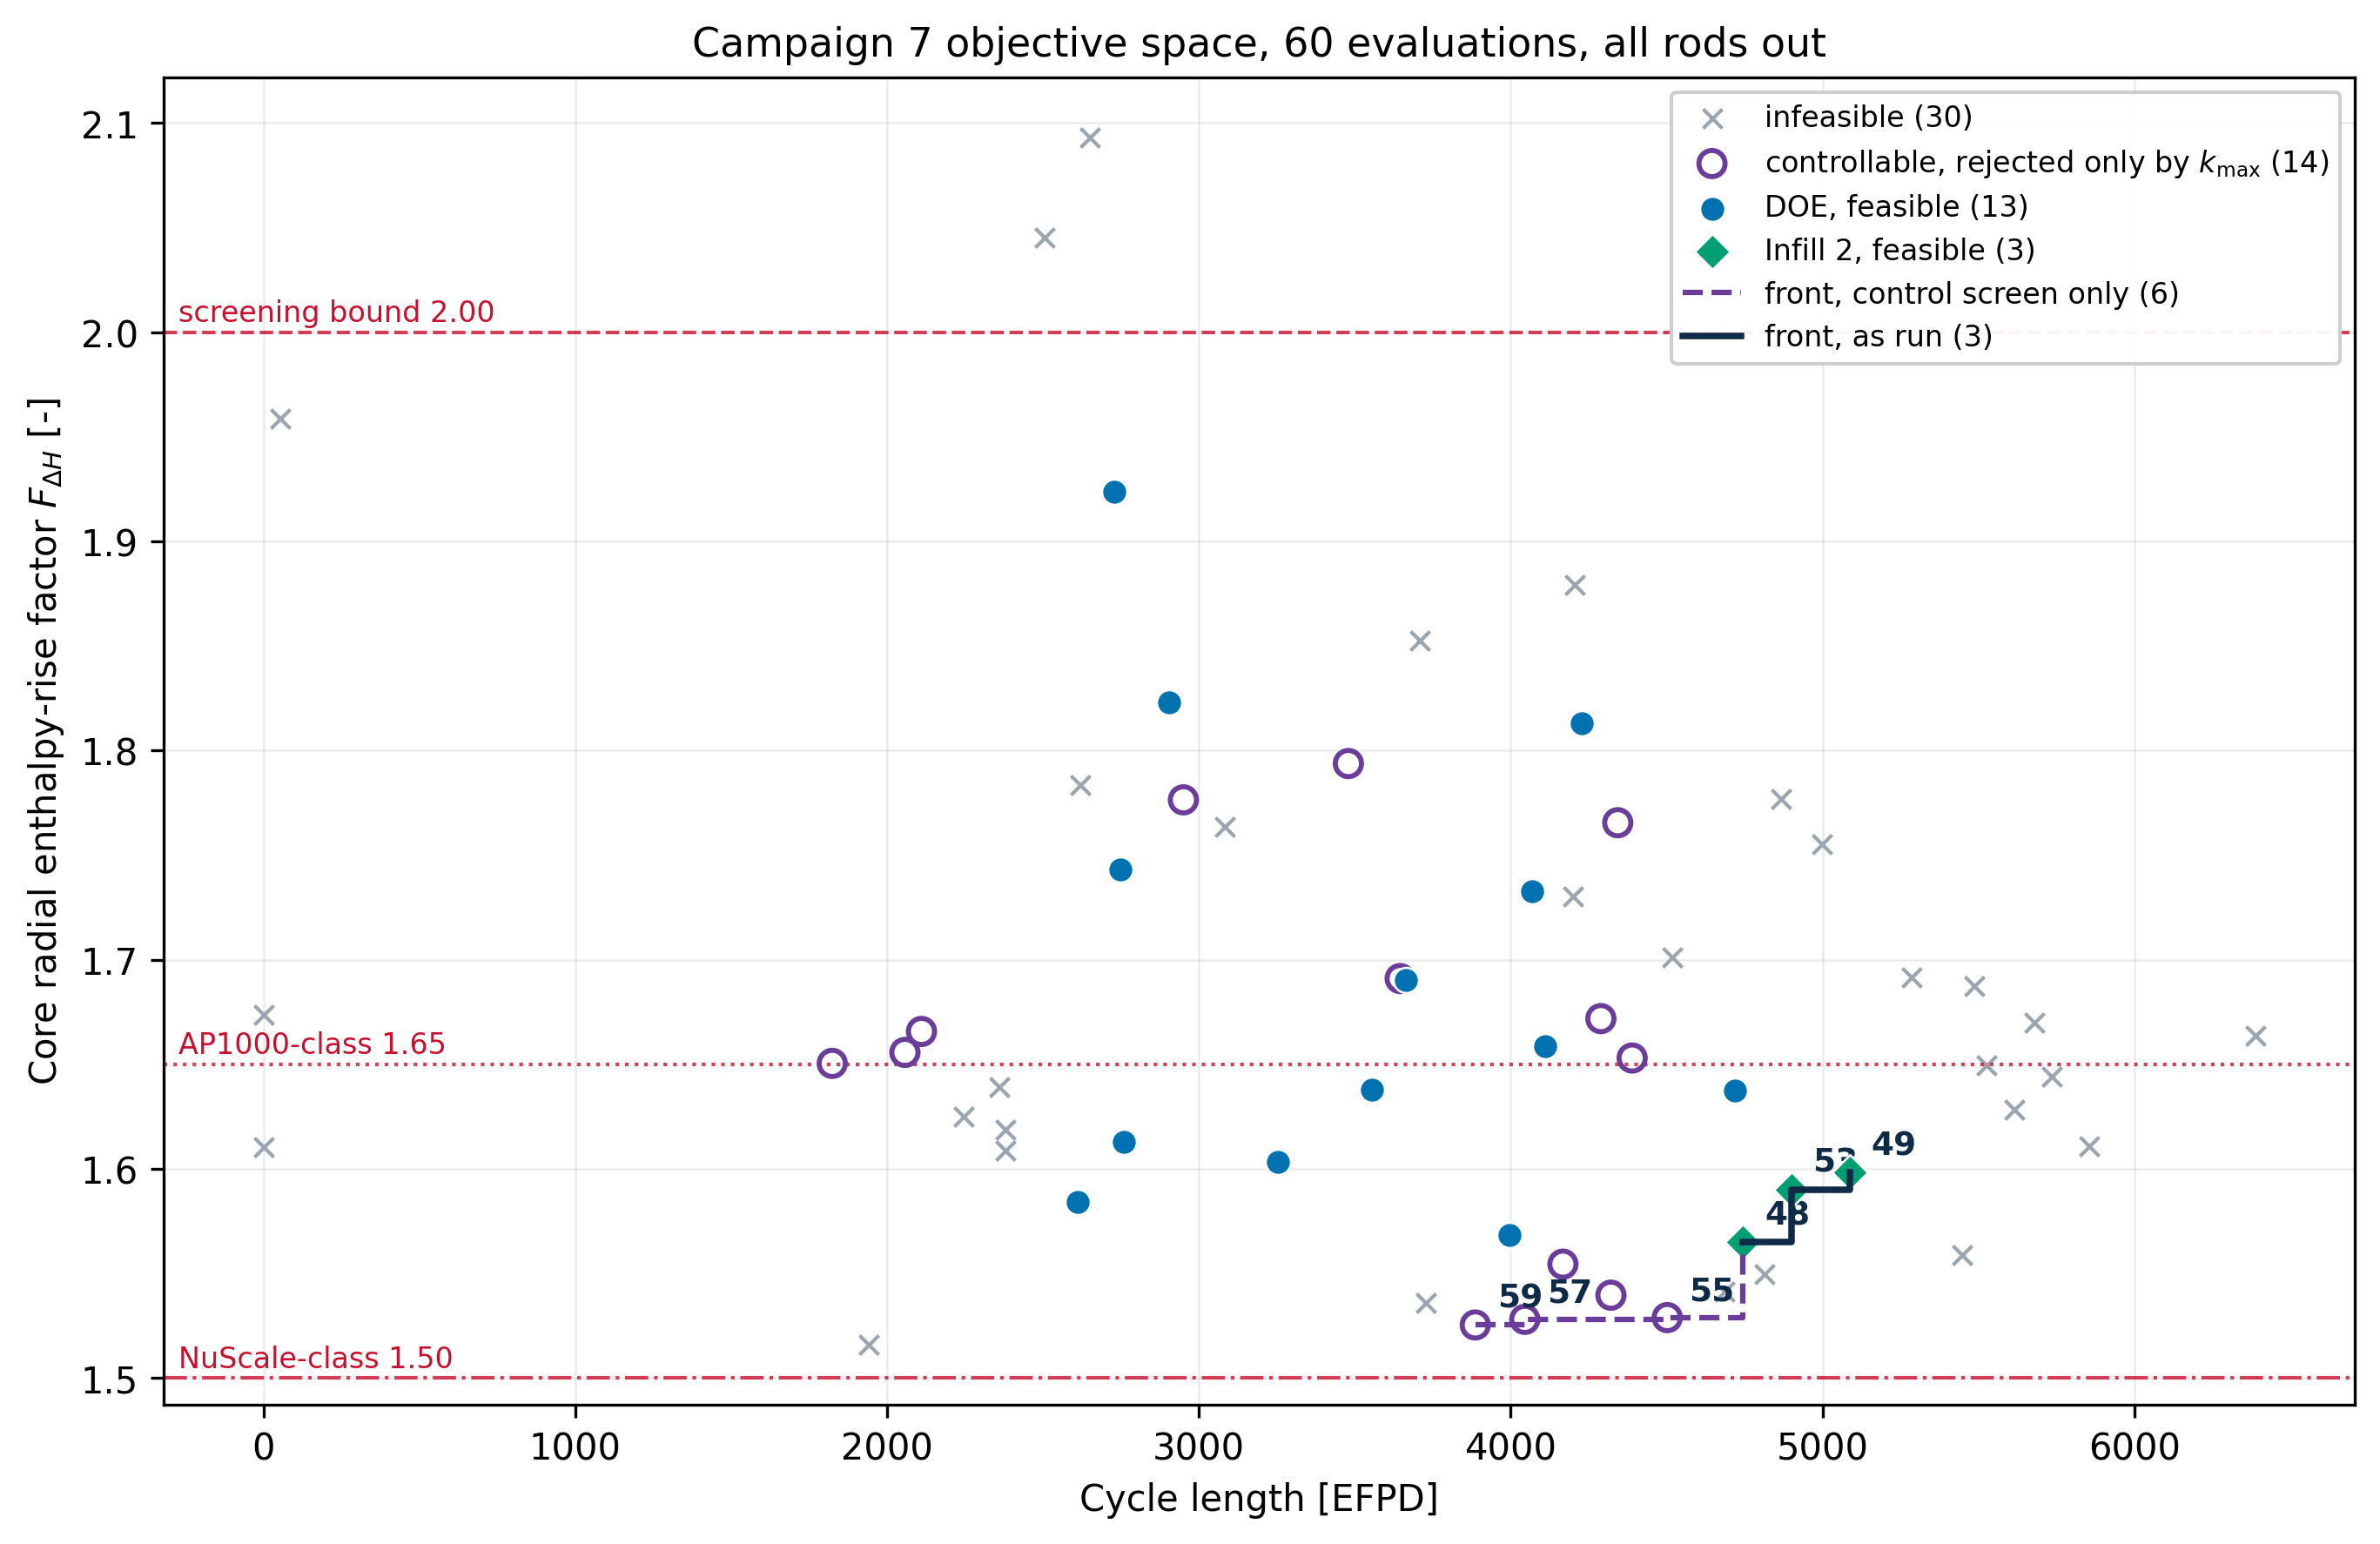
\includegraphics[width=\linewidth]{images/c7_pareto_60}
  \caption{Campaign 7 objective space with all rods out. Filled markers
  are feasible as run, open circles are controllable designs rejected
  only by the derived ceiling. The solid front is the one the campaign
  reported and the dashed front is the one the measured control screen
  supports.}
  \label{fig:c7-pareto}
\end{figure}

Two properties of the front as run deserve stating. Its three designs
sit \num{240} to \SI{680}{pcm} below the ceiling, so the front is a
constraint boundary and not an interior trade. And the cycle lengths
are not comparable with Campaign 6, because the enrichment box is a
different one, and the longest feasible cycle of 5087 EFPD says nothing
about the reactor class that the 9981 EFPD of Campaign 6 did not
already say.

%% AUTHOR: one paragraph on why the low-peaking end of the control-screen
%% front lives at thick reflectors and narrow pitch, and on the physical
%% meaning of a front that doubles when a surrogate bound is removed.

\subsection{Regulating-bank worth and the reason the screens nest}
\label{sec:res-c7-worth}

The worth of the sixteen regulating banks is defined on the two core
solves of every evaluation.

\begin{equation}
\rho_\mathrm{bank}(\mathbf{x}) = k_\mathrm{eff}^\mathrm{core}(\mathbf{x}) - k_\mathrm{ARI}(\mathbf{x})
\label{eq:bank-worth}
\end{equation}

\noindent where the symbols have the following meaning.

\begin{itemize}
  \item $\rho_\mathrm{bank}$ is the bank worth in units of $k$,
        dimensionless, reported in pcm by multiplying by $10^5$.

  \item $k_\mathrm{eff}^\mathrm{core}$ is the unrodded core eigenvalue
        at beginning of life, dimensionless.

  \item $k_\mathrm{ARI}$ is the eigenvalue with all sixteen regulating
        banks inserted, dimensionless.
\end{itemize}

Across the archive the worth ranges from \num{10936} to
\SI{22699}{pcm} with a median of \SI{16510}{pcm}. Figure~\ref{fig:c7-worth}
shows its two strongest drivers and Figure~\ref{fig:c7-influence} the
rank correlations of all six variables with the objectives, the worth
and the rodded peaking.

\begin{figure}[htbp]
  \centering
  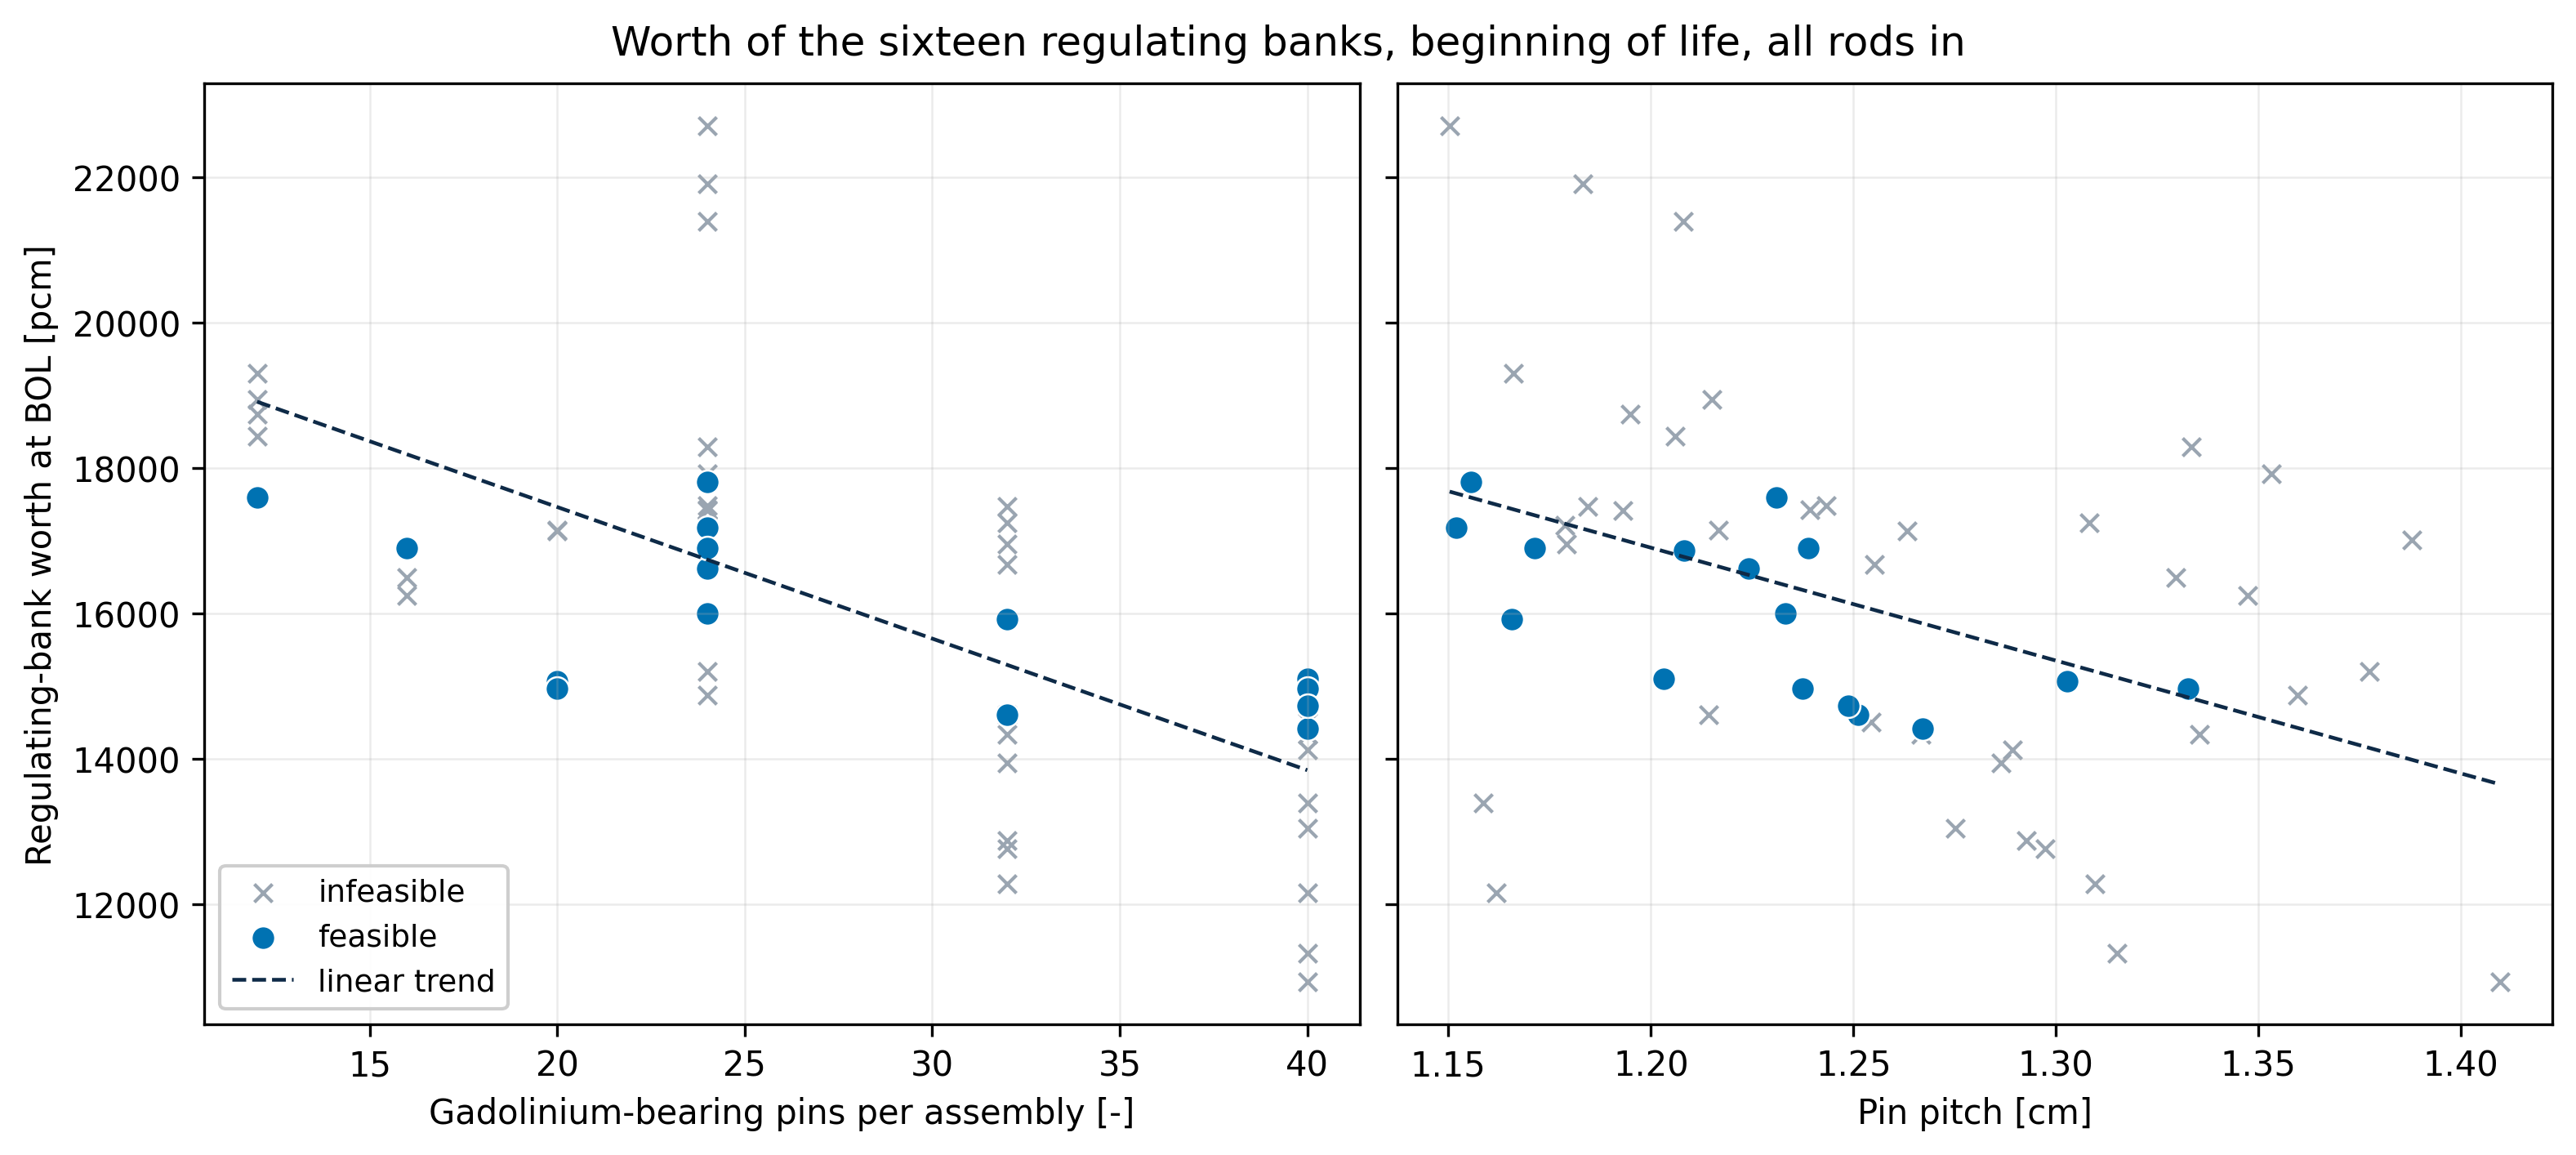
\includegraphics[width=\linewidth]{images/c7_rod_worth}
  \caption{Worth of the sixteen regulating banks against the
  gadolinium pin count and the pin pitch. The dashed lines are
  least-squares trends and serve only as visual guides.}
  \label{fig:c7-worth}
\end{figure}

\begin{figure}[htbp]
  \centering
  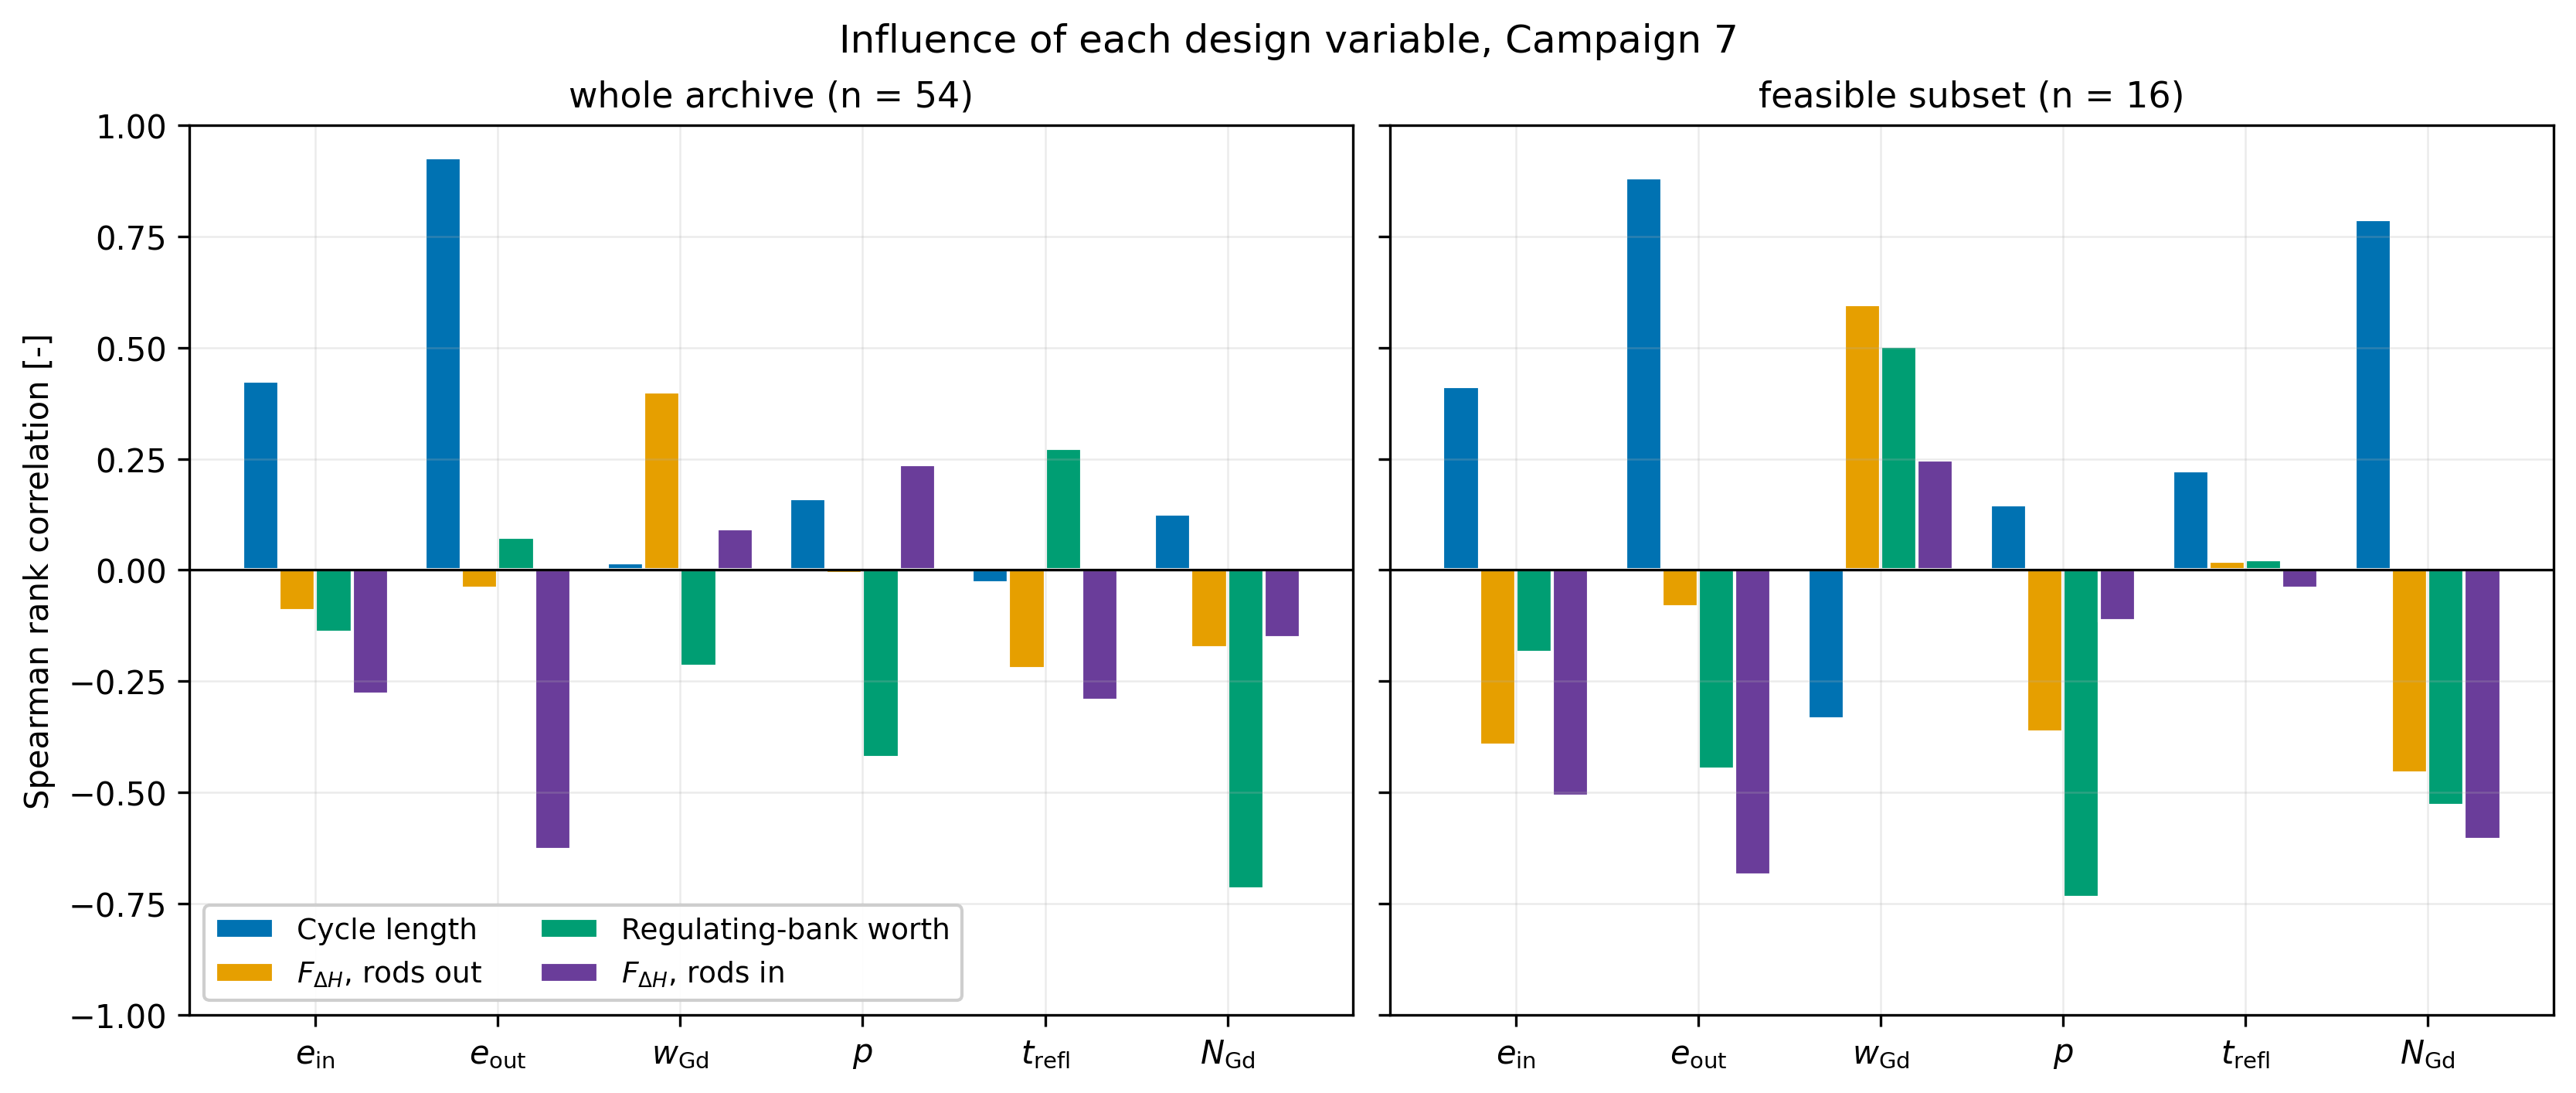
\includegraphics[width=\linewidth]{images/c7_vars_influence}
  \caption{Spearman rank correlation of each design variable with the
  two objectives, the regulating-bank worth and the peaking with the
  banks inserted, over the whole archive and over the feasible subset.}
  \label{fig:c7-influence}
\end{figure}

The worth correlates at $-0.68$ with the gadolinium pin count, at
$-0.45$ with the pitch and at $+0.61$ with the unrodded eigenvalue.
Gadolinium depresses the eigenvalue and the bank worth together, so the
designs with the least worth are the heavily poisoned ones, which are
already far below the ceiling for a different reason. That is why the
two screens nest in this design space, and it is also why the
eight-design derivation of the ceiling looked safe when it was not.
The eight designs were all high-enrichment, forty-pin designs from one
corner of the Campaign 6 front, and their worths were alike because
their poison inventories were alike.

The measurement also settles a question left open since Campaign 4.
The ceiling of 1.35 used in Campaigns 1 to 6 was described as a
screening value not traceable to a primary source. Deriving the
ceiling from the worth of all seven banks, that is all 32 control rod
assemblies, with the same \SI{1000}{pcm} margin gives 1.368. The value
used through six campaigns sits two per cent below the measured
all-bank controllability bound of this core. It is a measured quantity
in retrospect, and the methodology chapter now states it as such,
with the caveat that an all-bank insertion with a \SI{1000}{pcm}
operating margin is not a licensing shutdown margin, which also
requires the highest-worth assembly stuck out and the cold, xenon-free
state.

\subsection{Peaking with the regulating banks inserted}
\label{sec:res-c7-rodded}

The peaking objective is evaluated with all rods out. The same core
solve that measures $k_\mathrm{ARI}$ also yields the radial peaking
with the sixteen banks inserted, and Figure~\ref{fig:c7-rodded} plots
the two against each other.

\begin{figure}[htbp]
  \centering
  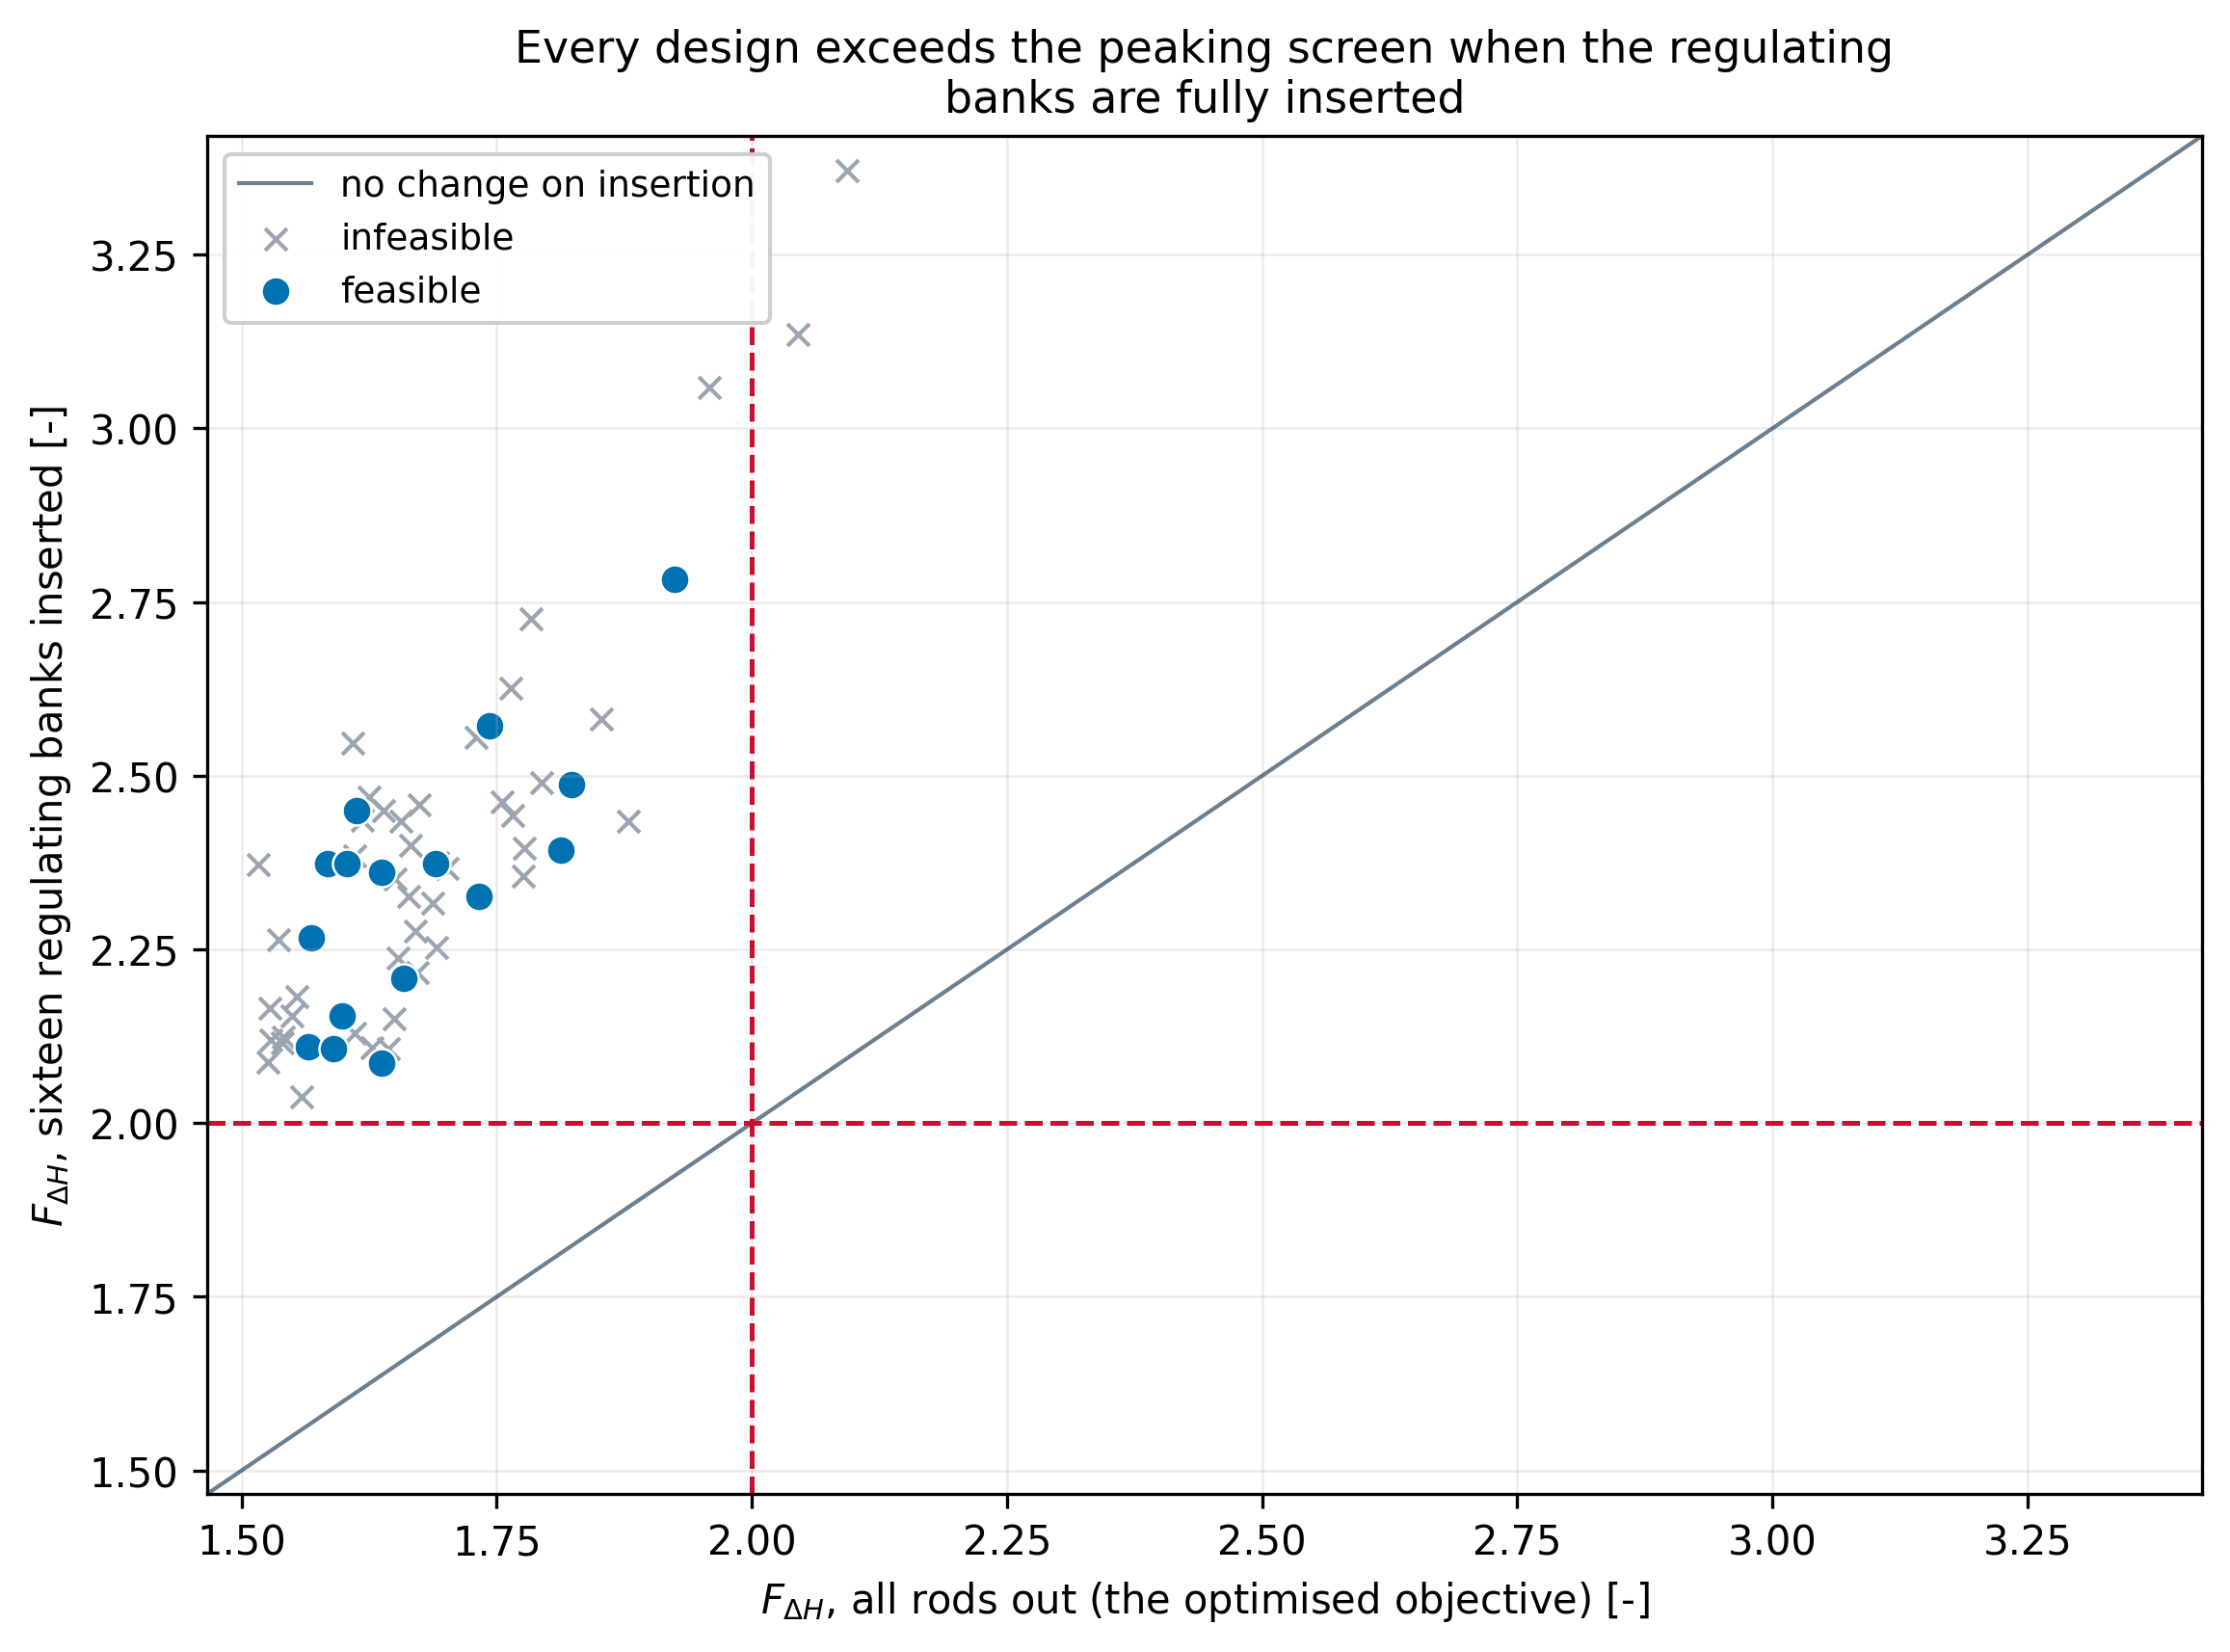
\includegraphics[width=0.85\linewidth]{images/c7_rodded_peaking}
  \caption{Radial peaking with all rods out, the optimised objective,
  against the same quantity with the sixteen regulating banks inserted.
  Every design lies above the screening bound of 2.0 in the rodded
  configuration.}
  \label{fig:c7-rodded}
\end{figure}

With the banks inserted $F_{\Delta H}$ runs from 2.038 to 3.371 with a
mean of 2.375, against 1.516 to 2.093 unrodded. The insertion penalty
ranges from 0.449 to 1.278 and is design dependent, correlating at
$-0.81$ with the outer-zone enrichment over the archive. Every one of
the 60 designs exceeds the screening bound of 2.0 in the rodded
configuration, and the three front designs sit between 2.11 and 2.16.

Two framings are required and neither should be overstated. Sixteen
banks fully inserted is the extreme of the regulating band used here as
a controllability test, not an operating configuration, so the rodded
value is an upper bound on operating peaking rather than an operating
value. Even so, the objective being minimised moves by half a unit or
more when the rods go in, and it moves by a design-dependent amount.
A design selected for low unrodded peaking is not thereby a design
with low rodded peaking. This is recorded as a limitation of the
objective set and as the motivation for the two-level reading of
Campaign 8.

%% AUTHOR: physical interpretation of the negative correlation between
%% the insertion penalty and the outer-zone enrichment.

\subsection{Depletion histories and the statistical error on the cycle length}
\label{sec:res-c7-uncertainty}

The assembly depletion solves are the only transport runs whose output
reaches the campaign log, and the log therefore holds the complete
$k_\infty(B)$ history of every design. Figure~\ref{fig:c7-histories}
reconstructs all 60 histories with the end-of-cycle crossing marked.

\begin{figure}[htbp]
  \centering
  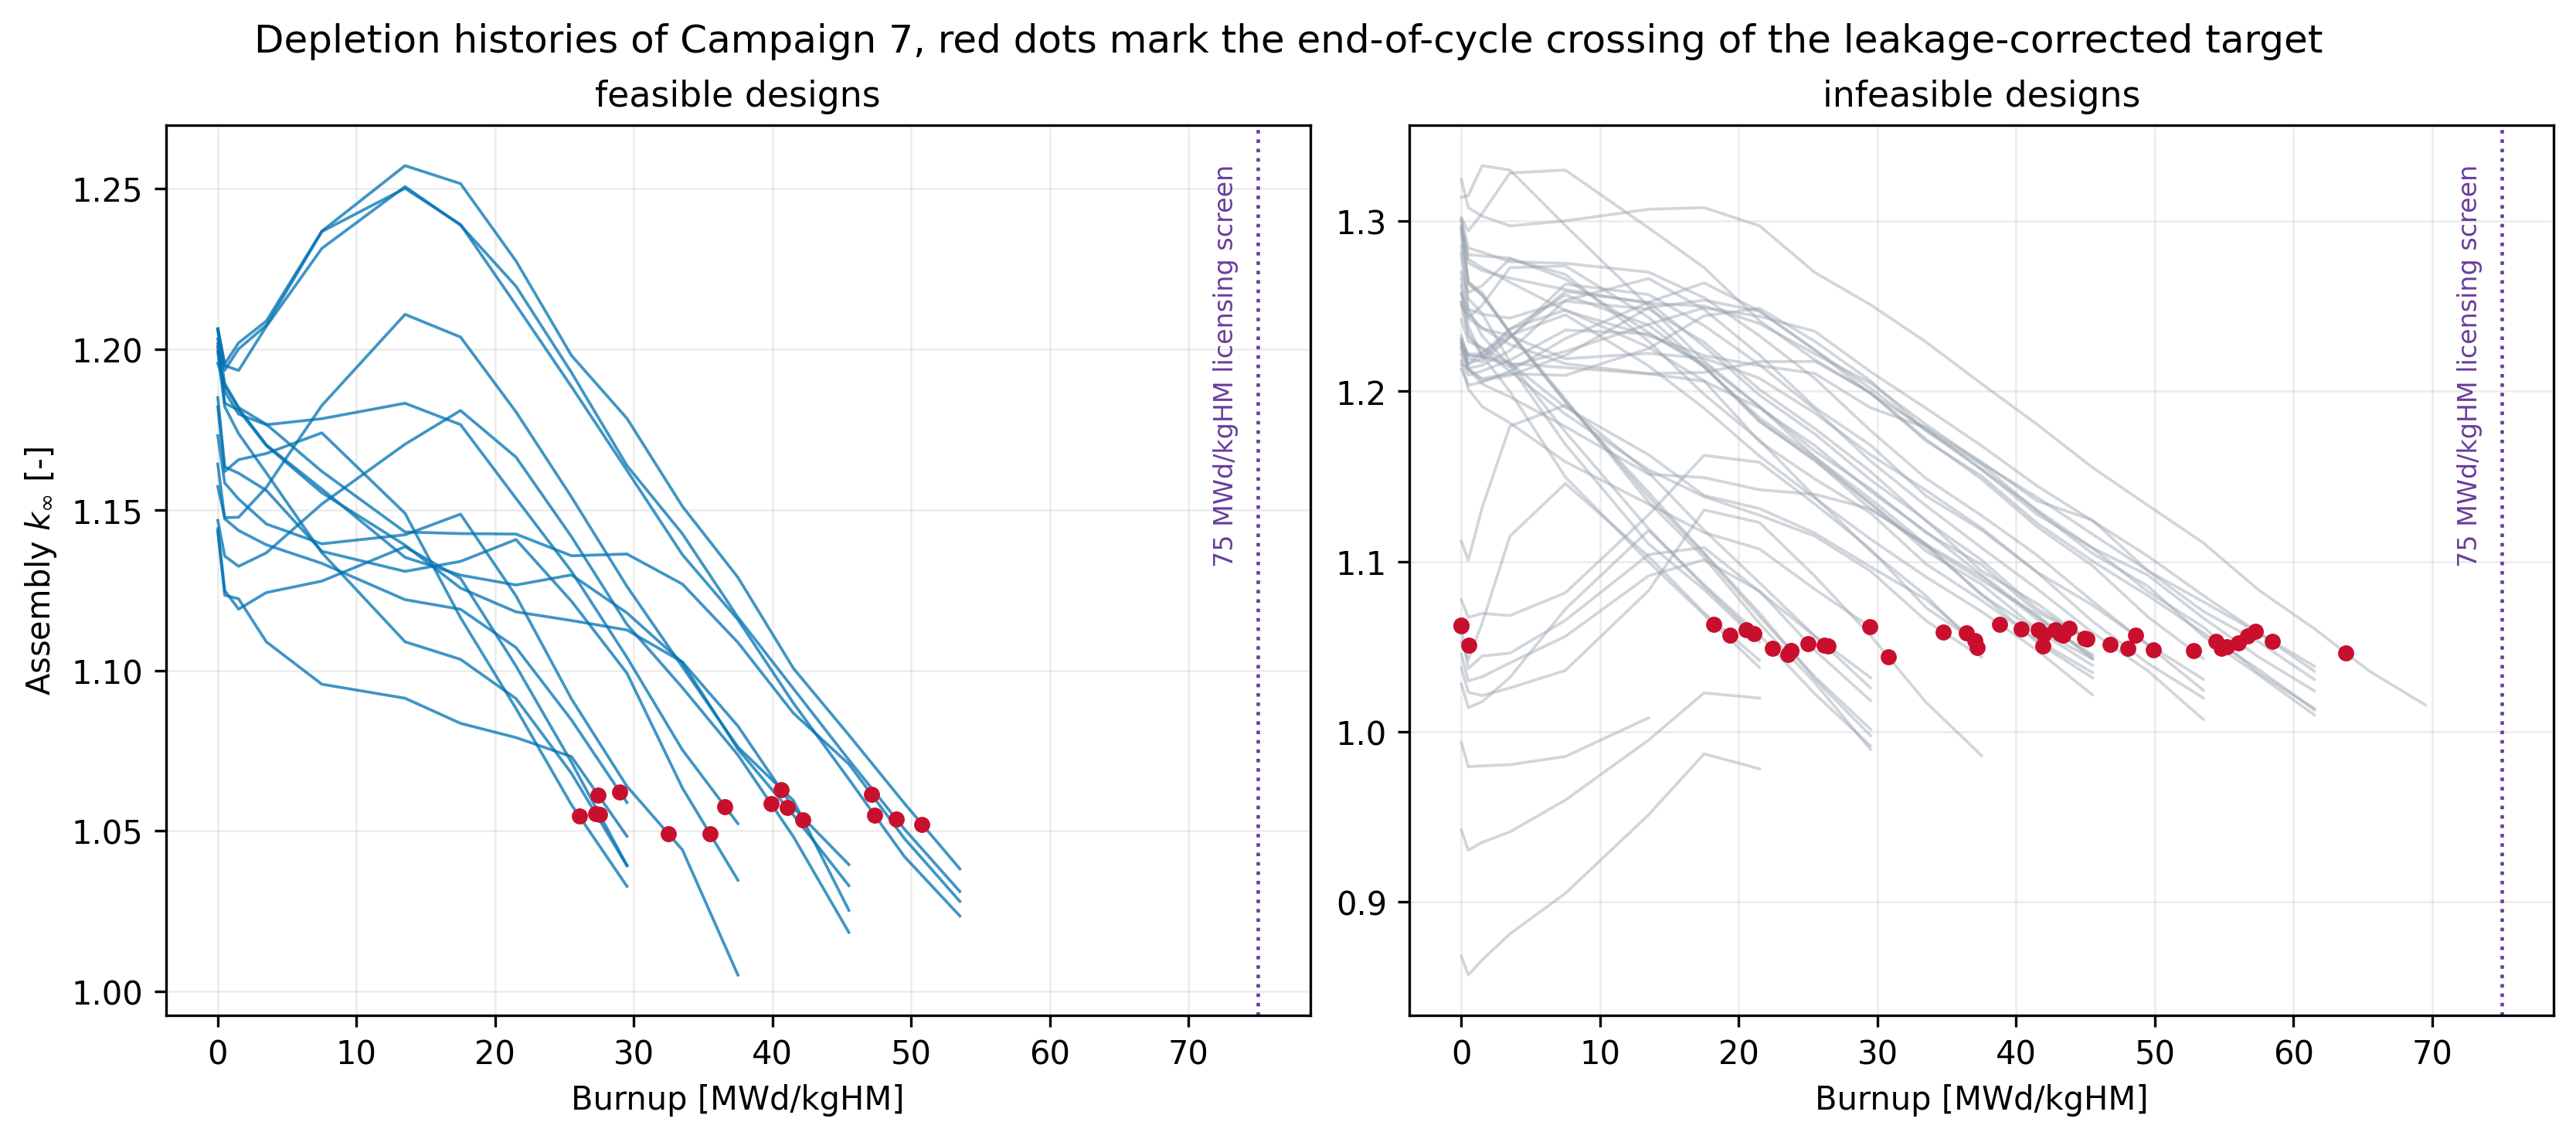
\includegraphics[width=\linewidth]{images/c7_kinf_histories}
  \caption{Assembly infinite multiplication factor against burnup for
  every Campaign 7 design, feasible designs on the left. Red markers
  are the end-of-cycle crossings of the leakage-corrected target. The
  gadolinium burnout maximum is visible between 13 and
  \SI{17}{MWd/kgHM}, and no design approaches the \SI{75}{MWd/kgHM}
  screen.}
  \label{fig:c7-histories}
\end{figure}

The reconstruction was validated against the archive. Taking the last
descending crossing of the target reproduces the stored end-of-cycle
burnup of all 57 crossing designs to within \SI{0.0011}{MWd/kgHM}. The
last crossing is the correct rule because the gadolinium burnout makes
the early history non-monotonic. The three designs without a crossing
are the two subcritical cores at zero cycle length and one design
ending at 55 EFPD.

Three facts follow from the figure. The gadolinium hump raises
$k_\infty$ by up to 0.06 before the decline. The highest end-of-cycle
burnup in the campaign is \SI{63.8}{MWd/kgHM}, so the
\SI{75}{MWd/kgHM} discharge screen of Section~\ref{sec:meth-atf} is
inactive and no design is censored, unlike Campaign 6. And the local
slope at end of cycle is steep, which governs the statistical error on
the cycle length.

The Monte Carlo error on the cycle length is obtained by propagating
the uncertainties of the two transport states that bracket the
crossing.

\begin{equation}
\sigma_B^2 = \left(\frac{\Delta B\,(k_\mathrm{t} - k_{j+1})}{(k_j - k_{j+1})^2}\right)^2 \sigma_{k_j}^2
+ \left(\frac{\Delta B\,(k_j - k_\mathrm{t})}{(k_j - k_{j+1})^2}\right)^2 \sigma_{k_{j+1}}^2
\label{eq:sigma-beoc}
\end{equation}

\noindent where the symbols have the following meaning.

\begin{itemize}
  \item $\sigma_B$ is the statistical uncertainty of the end-of-cycle
        burnup, in MWd/kgHM.

  \item $\Delta B$ is the burnup step between the two bracketing
        states, in MWd/kgHM.

  \item $k_j$ and $k_{j+1}$ are the infinite multiplication factors at
        the states before and after the crossing, dimensionless.

  \item $k_\mathrm{t}$ is the leakage-corrected target, dimensionless,
        treated as exact.

  \item $\sigma_{k_j}$ and $\sigma_{k_{j+1}}$ are the reported Monte
        Carlo standard deviations of the two states, dimensionless.
\end{itemize}

The cycle length follows from the specific power.

\begin{equation}
\sigma_\mathrm{EFPD} = \frac{1000\,\sigma_B}{P_\mathrm{sp}}
\label{eq:sigma-efpd}
\end{equation}

\noindent where the symbols have the following meaning.

\begin{itemize}
  \item $\sigma_\mathrm{EFPD}$ is the statistical uncertainty of the
        cycle length, in effective full power days.

  \item $P_\mathrm{sp}$ is the specific power of the core,
        \SI{9.98}{W/gHM}.
\end{itemize}

\begin{figure}[htbp]
  \centering
  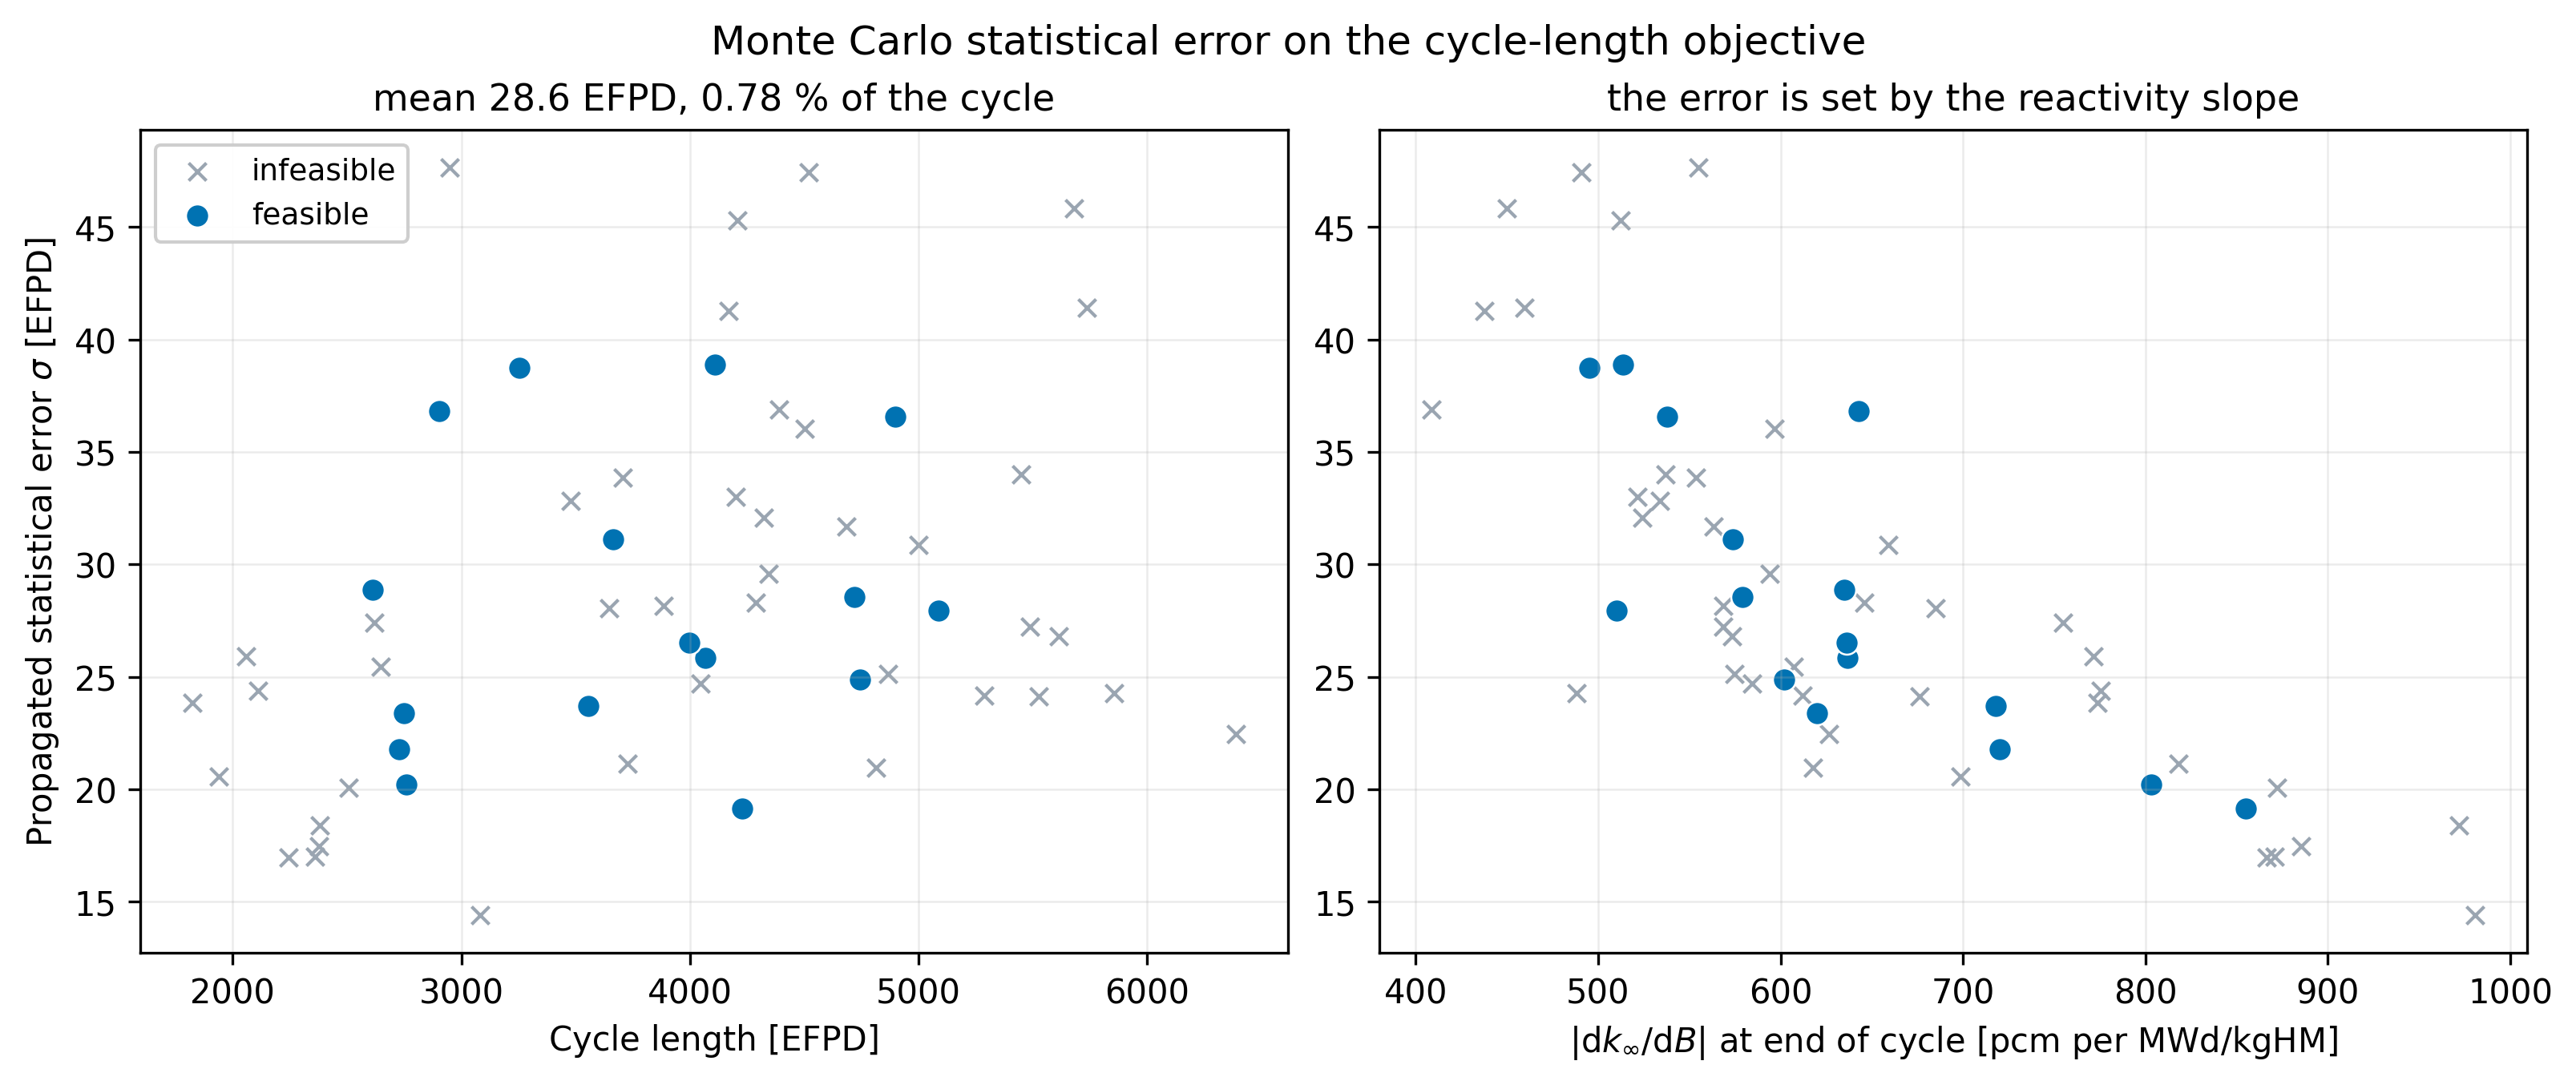
\includegraphics[width=\linewidth]{images/c7_cycle_uncertainty}
  \caption{Propagated Monte Carlo error on the cycle length against the
  cycle length and against the reactivity slope at end of cycle. The
  error is set by the slope, not by the length of the cycle.}
  \label{fig:c7-uncertainty}
\end{figure}

Table~\ref{tab:c7-uncertainty} summarises the result and
Figure~\ref{fig:c7-uncertainty} shows it. The slope at end of cycle
lies between 409 and \SI{981}{pcm} per MWd/kgHM with a median of 607.
The resulting error has a mean of 28.6 EFPD, \SI{0.78}{\%} of the
cycle, and a worst case of 47.7 EFPD, \SI{1.62}{\%}. On the six front
designs it is 25 to 37 EFPD. The smallest gap between adjacent front
designs is 154 EFPD, about five standard deviations, so the ordering of
the front in cycle length is statistically resolved.

\begin{table}[htbp]
  \centering
  \caption{Statistical error on the cycle length over the 57 designs
  with a resolved end-of-cycle crossing.}
  \label{tab:c7-uncertainty}
  \begin{tabular}{lccc}
    \toprule
    Quantity & Minimum & Median & Maximum \\
    \midrule
    Slope at end of cycle [pcm per MWd/kgHM] & 409 & 607 & 981 \\
    Bracketing sigma on $k_\infty$ [pcm]     & 178 & 218 & 274 \\
    $\sigma_\mathrm{EFPD}$ [d]               & 14.4 & 27.2 & 47.7 \\
    $\sigma_\mathrm{EFPD}$ as a fraction of the cycle [\%] & 0.35 & 0.74 & 1.62 \\
    \bottomrule
  \end{tabular}
\end{table}

The peaking axis is the opposite case. The front designs are separated
by 0.003 to 0.036 in $F_{\Delta H}$, the entropy study of
Section~\ref{sec:res-c6} bounded the systematic shift at $\pm 0.02$,
and no statistical error on the core peaking tally has been measured.
The ordering of the front in peaking is therefore not resolved, and
designs 59, 57 and 55 at 1.525, 1.528 and 1.529 must be treated as
indistinguishable until the tally errors are read from the statepoints.

\openpoint{Measure $\sigma(F_{\Delta H})$ from the per-bin relative
errors of the core mesh tally on the six front designs, or by seed
replicates, before any ordering claim on the peaking axis is made.}

\subsection{Cost and instrumentation}
\label{sec:res-c7-cost}

The campaign cost \SI{56965}{s} of wall time, \SI{949}{s} per
evaluation, against \SI{840}{s} in Campaign 6. The difference is the
control solve. Two instrumentation defects were found while reading
the archive, and both are recorded because they affect numbers reported
elsewhere in this chapter.

\begin{enumerate}
  \item The per-evaluation cost stored in the archive excludes the
        control solve, because that solve is invoked after the three
        timers close. Over the campaign the control solves are
        \SI{11}{\%} of the true cost and \SI{12.6}{\%} of the reported
        cost. The wall-clock figure of the block log is correct and is
        the one quoted above. The evaluator is corrected from Campaign
        8 (Section~\ref{sec:meth-cost}).

  \item The per-case parser of the run log never matched a single case
        line of any campaign, because the censoring marker inserted
        after the cycle length was not anticipated by its regular
        expression. The failure was silent, and every per-case table
        the parser produced before the correction was empty. No number
        in this chapter depends on that table, since all per-design
        quantities are read from the archive.
\end{enumerate}

\subsection{Limitations and what carries forward}
\label{sec:res-c7-limits}

Four limitations bound the claims of this section.

\begin{enumerate}
  \item Four designs, 10, 32, 41 and 43, reached the active batches
        with the Shannon entropy of the fission source not yet
        converged, the worst at 105 of 60 inactive batches. None is on
        either front. Their eigenvalues and peaking values carry an
        unquantified bias, are retained in the archive statistics of
        this section with that caveat, and are excluded from any
        candidate list.

  \item Twenty-five of the 60 designs have a pitch below
        \SI{1.2242}{cm}, twice the guide-tube outer radius. Below that
        value the lattice clips the guide-tube wall at the cell
        boundary silently, replacing up to \SI{27}{\%} of the wall
        cross-section by moderator at the box minimum of
        \SI{1.150}{cm}. Designs 57 and 59, the two lowest-peaking
        designs of the control-screen front, are both in the affected
        band. The same defect reaches back to every earlier campaign
        design at pitches below \SI{1.2242}{cm}, including the
        Campaign 4 infill designs pinned at the box minimum and the
        Campaign 6 discharge-screen champion at \SI{1.150}{cm}. Fixing
        the pitch at \SI{1.26}{cm} in Campaign 8 removes the defect
        prospectively, and a caveat is added to the affected results.

  \item The statistical error on the peaking objective is not
        measured, as stated above.

  \item Every cycle length in this campaign, as in all earlier ones, is
        a two-dimensional value. The axial leakage study of
        Section~\ref{sec:meth-lax}, completed after this campaign,
        measured the axial correction at \num{1.0282} to \num{1.0298}
        on six Campaign 6 designs, about \SI{3000}{pcm} of reactivity,
        which at the end-of-cycle slopes measured here corresponds to
        roughly 450 to 500 EFPD. Campaign 7 cycle lengths are therefore
        overstated by that amount relative to a finite-height core,
        uniformly across the archive, and the ordering of the front is
        unaffected. Campaign 8 carries the correction inside the
        end-of-cycle target from the start.
\end{enumerate}

What carries forward is the constraint architecture. The measured
control screen replaces the derived ceiling as the reactivity
constraint that does the work, a second reading with only the first two
banks inserted is added and recorded, the axial factor enters the
target, the acquisition settings of Campaign 6 are restored explicitly,
and the pitch is fixed at the value that both closes the geometric
defect and matches the reference fuel design. Section~\ref{sec:res-c8}
states the campaign built on those decisions.
